% file: DGDT_dump.tex
% Differential Geometry, Differential Topology, in unconventional ``grande'' format; fitting a widescreen format
% 
% github        : ernestyalumni
% linkedin      : ernestyalumni 
% wordpress.com : ernestyalumni
%
% This code is open-source, governed by the Creative Common license.  Use of this code is governed by the Caltech Honor Code: ``No member of the Caltech community shall take unfair advantage of any other member of the Caltech community.'' 
% 

\documentclass[10pt]{amsart}
\pdfoutput=1
%\usepackage{mathtools,amssymb,lipsum,caption}
\usepackage{mathtools,amssymb,caption}

\usepackage{graphicx}
\usepackage{hyperref}
\usepackage[utf8]{inputenc}
\usepackage{listings}
\usepackage[table]{xcolor}
\usepackage{pdfpages}
%\usepackage[version=3]{mhchem}
%\usepackage{mhchem}

\usepackage{tikz}
\usetikzlibrary{matrix,arrows}

\usepackage{multicol}

\hypersetup{colorlinks=true,citecolor=[rgb]{0,0.4,0}}

\oddsidemargin=15pt
\evensidemargin=5pt
\hoffset-45pt
\voffset-55pt
\topmargin=-4pt
\headsep=5pt
\textwidth=1120pt
\textheight=595pt
\paperwidth=1200pt
\paperheight=700pt
\footskip=40pt








\newtheorem{theorem}{Theorem}
\newtheorem{corollary}{Corollary}
%\newtheorem*{main}{Main Theorem}
\newtheorem{lemma}{Lemma}
\newtheorem{proposition}{Proposition}

\newtheorem{definition}{Definition}
\newtheorem{remark}{Remark}

\newenvironment{claim}[1]{\par\noindent\underline{Claim:}\space#1}{}
\newenvironment{claimproof}[1]{\par\noindent\underline{Proof:}\space#1}{\hfill $\blacksquare$}

%This defines a new command \questionhead which takes one argument and
%prints out Question #. with some space.
\newcommand{\questionhead}[1]
  {\bigskip\bigskip
   \noindent{\small\bf Question #1.}
   \bigskip}

\newcommand{\problemhead}[1]
  {
   \noindent{\small\bf Problem #1.}
   }

\newcommand{\exercisehead}[1]
  { \smallskip
   \noindent{\small\bf Exercise #1.}
  }

\newcommand{\solutionhead}[1]
  {
   \noindent{\small\bf Solution #1.}
   }


\title{The Differential Geometry Differential Topology Dump}
\author{Ernest Yeung \href{mailto:ernestyalumni@gmail.com}{ernestyalumni@gmail.com}}
\date{28 juillet 2016}
\keywords{Differential Geometry, Differential Topology}
\begin{document}

\definecolor{darkgreen}{rgb}{0,0.4,0}
\lstset{language=Python,
 frame=bottomline,
 basicstyle=\scriptsize,
 identifierstyle=\color{blue},
 keywordstyle=\bfseries,
 commentstyle=\color{darkgreen},
 stringstyle=\color{red},
 }
%\lstlistoflistings

\maketitle



\begin{multicols*}{2}

  
\setcounter{tocdepth}{1}
\tableofcontents



\begin{abstract}
Everything about Differential Geometry, Differential Topology

\end{abstract}

\part{Combinatorics, Probability Theory}

\begin{theorem}[4.2. of Feller (1968)  \cite{Fell1968}]
	Let $r_1,\dots r_k \in \mathbb{Z}$, s.t. $r_1 + r_2 + \dots + r_k = n$;, $r_i \geq 0$.  

Let 
\begin{equation}
\frac{ N! }{r_1! r_2! \dots r_k!} = 
\end{equation}
number of ways in which $n$ elemnts can be divided into $k$ ordered parts (partitioned into $k$ subpopulations).  cf. Eq. (4.7) of Feller (1968)  \cite{Fell1968}.  

Note that the order of the subpopulations is essential in the sense that ($r_1 = 2,r_2 =3$) and ($r_1=3,r_2=2$) represent different partitions.  However, no attention is paid to the order within the groups.  

\end{theorem}
\begin{proof}
\begin{equation}
\binom{n}{r_1} \binom{n-r_1}{r_2} \binom{n-r_1-r_2}{r_3} \dots \binom{n-r_1-\dots - r_{k-2} }{ r_{k-1} } = \frac{n!}{ r_1! r_2! \dots r_k! }
\end{equation}
i.e. in order to effect the desired partition, we have to select $r_1$ elementsout of $n$, remaining $n-r_1$ elements select a second group of size $r_2$, etc.  After forming the $(k-1)$st group there remains $n-r_1 -r_2 - \dots - r_{k-1} = r_k$ elements, and these form the last group.  
\end{proof}

cf. pp. 37 of Feller (1968)  \cite{Fell1968}
Examples.  (g) Bridge.  32 cards are partitioned into 4 equal groups $\to 52!/(13!)^4$.  

Probability each player has an ace (?).  

The 4 aces can be ordered in $4! = 24$ ways, each order presents 1 possibility of giving 1 ace to each player.  \\
Remaining 48 cards distributed $(48!)/( 12!)^4$ ways.  

\[
\to p = 24 \frac{ 48!}{ (12!)^4 } / \frac{ 52!}{ (13!)^4}
\]

(h) A throw of 12 dice $\to  6^{12}$ different outcomes total.  Event each face appears twice can occur in as many ways as 12 dice can be arranged in 6 groups of 2 each.  
\[
\frac{12!}{(2!)^6} / \frac{ 52!}{ (13!)^4} 
\]

\subsubsection{Application to Occupancy Problems; binomial coefficients}

cf. Sec. 5 Application to Occupancy Problems of Feller (1968)  \cite{Fell1968}.  

Consider randomly placing $r$ balls intos $n$ cells.  

Let $r_k = $ occupancy number $=$ number of balls in $k$th cell.  

Every $n$-tuple of integers satisfying $r_1 + r_2 + \dots + r_n = r$;  $r_k \geq 0$.  describes a possible configuration of occupancy numbers.  

With indistinguishable balls 2 distributions are distinguishable only if the corresponding $n$-tuples ($r_1,\dots r_n$) are not identical.  

\begin{enumerate}
\item[(i)] number of distinguishable distributions is 
\begin{equation}
A_{r,n} = \binom{n+r-1}{r} = \binom{n+r-1}{n-1}  
\end{equation} cf. Eq. (5.2) of Feller (1968)  \cite{Fell1968}
\item[(ii)]  number of distinguishable distributions in which no cell remains empty is $\binom{r-1}{n-1}$.  
\end{enumerate}

\begin{proof}
Represent balls by stars, indicate $n$ cells by $n$ spaces between $n+1$ bars.  e.g. $\begin{aligned} & \quad \\ 
& r= 8 \text{ balls } \\
& n = 6 \text{ cells } \end{aligned}$.  

\[
\begin{aligned}
	& 3 	  & 1   & 0 & 0 & 0 & 4 \\
	& | * * * & | * & | & |   & | & | **** |  
\end{aligned}
\]

Such a symbol necessarily starts and ends with a bar, but remaining $n-1$ bars and $r$ starts appear in an arbitrary order.  In this way, it becomes apparent that the number of distinguishable distributions equals the number of ways of selecting.  

$r$ places out of $n+r-1$, $\frac{ (n+r-1)! }{ (n-1)! r!} = \binom{n-1+r}{r} $  

\[
\begin{aligned}
	& | | | | \dots | | \qquad \, n+1 \text{ bars } \\ 
	& * * * \dots * * \qquad \, r \text{ stars leave } r-1 \text{ spaces }
\end{aligned}
\]

Condition that no cell be empty imposes the restriction that no 2 bars be adjacent.  $r$ stars leave $r-1$ spaces of which $n-1$ are to be occupied by bars.  Thus $\binom{r-1}{n-1}$ choices.  


\end{proof}


Probability to obtain given occupancy numbers $r_1,\dots r_n = \frac{r!}{ r_1! r_2! \dots r_n! } / n^r$, with $ \begin{aligned} & \quad \\ 
	& r \text{ balls } \\ 
& n \text{ cells } \end{aligned}$  given by Thm. 4.2. of Feller (1968)  \cite{Fell1968}, which is the Maxwell-Boltzmann distribution.  

\begin{enumerate}
\item[(a)] Bose-Einstein and Fermi-Dirac statistics.  Consider $r$ indistinguishable particles, $n$ cells, each particle assigned to 1 cell.  

State of the system - random distribution of $r$ particles in $n$ cells.  

If $n$ cells distinguishable, $n^r$ arrangements equiprobable $\to $ Maxwell-Boltzmann statistics.  

Bose-Einstein statistics: only distinguishable arrangements are considered, and each assigned probability $\frac{1}{A_{r,n}}$  
\begin{equation}
A_{r,n} = \binom{n+r-1}{r} = \binom{n-1+r}{n-1}  
\end{equation}
cf. Eq. 5.2 of Feller (1968)  \cite{Fell1968}

Fermi-Dirac statistics.  
\begin{enumerate}
\item[(1)] impossible for 2 or more particles to be in the same cell.  $\to r \leq n$.  
\item[(2)] all distinguishable arrangements satisfying the first condition have equal probabilities.  

$\to$ an arrangement is completely described by stating which of the $n$ cells contain a particle  

$r$ particles $\to \binom{n}{r}$ ways $r$ cells chosen.  

Fermi-Dirac statistics, there are $\binom{n}{r}$ possible arrangements, prob. $1/\binom{n}{r}$.  
\end{enumerate}
\end{enumerate}
pp. 39.  Feller (1968)  \cite{Fell1968}.  Consider cells themselves indistinguishable!  Disregard order among occupancy numbers.  








cf. Feller (1968)  \cite{Fell1968}




\part{Linear Algebra Review}

cf. \emph{Change of Basis}, of Appendix B of  John Lee (2012) \cite{JLee2012}.  

\exercisehead{B.22} Suppose $V,W, X$ finite-dim. vector spaces \\
$S:V\to W$, \, $T:W \to X$

\begin{enumerate}
	\item[(a)] $\text{rank}S \leq \text{dim}V$ \quad \, with $\text{rank}S = \text{dim}V$ iff $S$ injective
	\item[(b)] $\text{rank}S \leq \text{dim}W$ \quad \, with $\text{rank}S = \text{dim}W$ iff $S$ surjective
	\item[(c)] if $\text{dim}V = \text{dim}W$ and $S$ either injective or surjective, then $S$ isomorphism 
	\item[(d)] $\text{rank}TS \leq \text{rank}S$ \quad \, $\text{rank}TS = \text{rank}S$ iff $\text{im}S \bigcap \text{ker}T = 0$ 
	\item[(e)] $\text{rank}TS \leq \text{rank}T$ \quad \, $\text{rank}TS = \text{rank}T$ iff $\text{im}S + \text{ker}T = W$
	\item[(f)] if $S$ isomorphism, then $\text{rank}TS = \text{rank}T$
	\item[(g)] if $T$ isomorphism, then $\text{rank}TS = \text{rank}S$
\end{enumerate}

EY : Exercise B.22(d) is useful for showing the chart and atlas of a Grassmannian manifold, found in the More examples, for smooth manifolds.  

\begin{proof}
	\begin{enumerate}
		\item[(a)] Recall the \textbf{rank-nullity theorem}:  
		\begin{theorem}[Rank-Nullity Theorem] 
\begin{equation}
\text{dim}(\text{im}(S)) + \text{dim}(\text{ker}(S)) = \text{dim}V  
\end{equation}			
			\end{theorem} 
		Now
		\[
		\begin{gathered}
		\text{rank}(S) + \text{dim}(\text{ker}(S)) \equiv \text{dim}(\text{im}(S)) + \text{dim}(\text{ker}(S)) = \text{dim}V  \\
\Longrightarrow \boxed{ 	\text{rank}(S) \leq \text{dim}V  }
\end{gathered}
		\]
		
		If $\text{rank}(S) = \text{dim}{V}$, \\
		then by rank-nullity theorem, $\text{dim}(\text{ker}(S)) = 0$, implying that $\text{ker}S = \lbrace 0 \rbrace$.  \\
		Suppose $v_1, v_2 \in V$ and that $S(v_1) = S(v_2) $.  By linearity of $S$, $S(v_1) - S(v_2) = S(v_1-v_2) = 0$, which implies, since $\text{ker}S = \lbrace 0 \rbrace$, that $v_1 - v_2 = 0$.  \\
		$\Longrightarrow v_1 = v_2$.  Then by definition of injectivity, $S$ injective.  
		
		If $S$ injective, then $S(v)=0$ implies $v=0$.  Then $\text{ker}S = \lbrace 0 \rbrace$.  Then by rank-nullity theorem, $\text{rank}(S) = \text{dim}{V}$.  
		
		\item[(b)] 		$\forall \, w \in \text{im}(S)$, $w\in W$.  Clearly $\text{rank}S \leq \text{dim}W$.  
		
		If $S$ surjective, $\text{im}(S) = W$.  Then $\text{dim}(\text{im}(S)) = \text{rank}S = \text{dim}W$.  \\
		
		If $\text{rank}S = \text{dim}W = m$, then $\text{im}(S)$ has basis $\lbrace y_i \rbrace_{i=1}^m$, $y_i \in \text{im}(S)$, so $\exists \, x_i \in V$, $i=1\dots m$ s.t. $S(x_i) = y_i$, with $\lbrace S(x_i) \rbrace_{i=1}^m $ linearly independent.  
		
		Since $\lbrace S(x_i) \rbrace_{i=1}^m$ linearly independent and $\text{dim}W = m$, $\lbrace S(x_i) \rbrace_{i=1}^m$ basis for $W$.   \\
		$\forall \, w \in W$, $w=\sum_{i=1}^m w^i S(x_i) = S(\sum_{i=1}^m w^i x_i)$.  $\sum_{i=1}^m w^i x_i \in V$.  $S$ surjective.  
		
		\item[(c)]
		\item[(d)] Now 
		\[
		\begin{aligned}
		& \text{dim}V = \text{rank}TS + \text{nullity}TS \\ 
		&  \text{dim}V = \text{rank}S + \text{nullity}S
		\end{aligned}
		\]
		$\text{ker}S \subseteq \text{ker}TS$, clearly, so $\text{nullity}S \leq \text{nullity}TS$ 
		\[
		\Longrightarrow \boxed{ \text{rank}TS \leq \text{rank}S } 
		\]
		
		If $\text{rank}TS = \text{rank}S$, \\
		\phantom{ \quad } then $\text{nullity}S = \text{nullity}TS$ \\
		\phantom{ \, } Suppose $w \in \text{Im}S \bigcap \text{ker}T$, $w \neq 0$ \\
		\phantom{ \quad } Then $\exists \,  v\in S$, s.t. $w = S(v)$ and $T(w)=0$ \\
		\phantom{ \quad \, } Then $T(w) = TS(v) =0$.  So $v\in \text{ker}TS$ \\
		\phantom{ \quad \quad \, } $v\notin \text{ker}S$ since $w = S(v) \neq 0$ \\
		\phantom{ \quad \quad \, } This implies $\text{nullity}TS > \text{nullity}S$.  Contradiction. \\
		$\Longrightarrow \text{Im}S \bigcap \text{ker}T =0$ \\
		
		If $\text{Im}S \bigcap \text{ker}T =0$, \\
		\phantom{ \quad } Consider $v \in \text{ker}TS$.  Then $TS(v)=0$.  \\
		\phantom{ \quad  Consider $v \in \text{ker}TS$}.  Then $S(v)  \in \text{ker}T$ \\
		\phantom{ \quad  } $S(v) =0$; otherwise, $S(v) \in \text{Im}S$, contradicting given $\text{Im}S \bigcap \text{ker}T =0$ \\
		\phantom{ \quad \quad } $v\in \text{ker}S$ \\
		
		$\text{ker}TS \subseteq \text{ker}S$\\
		$\Longrightarrow \text{ker}TS = \text{ker}S$ \\
		So $\text{nullity}TS = \text{nullity}S$  \\
		$\Longrightarrow \text{rank}TS = \text{rank}S$ 
		
		\item[(e)]
		\item[(f)]
		\item[(g)]
	\end{enumerate}
\end{proof}


\part{Manifolds}


\section{Inverse Function Theorem}

Shastri (2011) had a thorough and lucid and explicit explanation of the Inverse Function Theorem \cite{AShastri2011}.  I will recap it here.  The following is also a blend of Wienhard's Handout 4 \url{https://web.math.princeton.edu/~wienhard/teaching/M327/handout4.pdf}

\begin{definition}
  Let $(X,a)$ metric space.  

\textbf{contraction} $\phi:X \to X$ if $\exists \, $ constant $0<c<1$ s.t. $\forall \, x,y \in X$
\[
d(\phi(x),\phi(y)) \leq cd(x,y)
\]
\end{definition}

\begin{theorem}[Contraction Mapping Principle]
  Let $(X,d)$ complete metric space.  \\
Then $\forall \, $ contraction $\phi:X\to X$, $\exists \, ! y\in X$ s.t. $\phi(y) = y$, $y$ \emph{fixed pt.}
\end{theorem}

\begin{proof}
  Recall def. of complete metric space $X$, $X$ metric space s.t. $\forall \, $ Cauchy sequence in $X$ is convergent in $X$ (i.e. has limit in $X$).  

$\forall \, x_0 \in X$,
Define $\begin{aligned} & \quad \\
  & x_1 = \phi(x_0) \\ 
  & x_2 = \phi(x_1) \\ 
  & \vdots \\
  & x_j = \phi(x_{j-1}) \\ 
  & \vdots \\
  & x_n = \phi(x_{n-1})
\end{aligned}$

\[
\begin{gathered}
  d(x_{n+1},x_n) = d(\phi(x_n),\phi(x_{n-1})) \leq c d(x_n,x_{n-1}) \leq \dots \leq c^nd(x_1,x_0)
\end{gathered}
\]
for some $0< c<1$.

\[
d(x_m,x_n) \leq d(x_n,x_{n-1}) + d(x_{n-1},x_m) \leq d(x_n,x_{n-1}) + d(x_{n-1},x_{n-2}) + \dots + d(x_{m+1},x_m) \leq \sum_{k=n-1}^m c^k d(x_1,x_0)
\]
Thus, $\forall \, \epsilon >0$, $\exists \, n_0 >0$, ($n_0$ large enough) s.t. $\forall \, m ,n\in \mathbb{N}$ s.t. $n_0 < n <m$, 
\[
d(x_m,x_n) \leq \sum_{k=n-1}^m c^k d(x_1,x_0) < \epsilon d(x_1,x_0)
\]
Thus, $\lbrace x_n \rbrace$ Cauchy sequence.  Since $X$ complete, $\exists \, $ limit pt. $y \in X$ of $\lbrace x_n \rbrace$.  
\[
\phi(y) = \phi(\lim_n x_n) = \lim_n \phi(x_n) = \lim_n x_{n+1} = y
\]
Since by def. of $y$ limit pt. of $\lbrace x_n \rbrace$, $\forall \, \epsilon >0$, then $\lbrace n | |x_n -y|\leq \epsilon, \, n \in \mathbb{N}\rbrace$ is infinite.  

Consider $\delta > \mathbb{N}$.  Consider $\lbrace n | |x_n-y| \leq \delta, n \in \mathbb{N}\rbrace$ 

$\exists \, N_{\delta} \in \mathbb{N}$ s.t. $\forall \, n > N_{\delta}$, $|x_n-y|< \delta$; otherwise, $\forall \, N_{\delta}$, $\exists \, n > N_{\delta}$ s.t. $|x_n - y| \geq \delta$.  Then $\lbrace n | |x_n -y| \leq \delta , n \in \mathbb{N} \rbrace$ finite.  Contradiction.  

$\phi$ cont. so by def. $\forall \, \epsilon >0$, $\exists \, \delta >0$ s.t. if $|x_n -y| < \delta$, then $|\phi(x_n) - \phi(y) | < \epsilon$.  

Pick $N_{\delta}$ s.t. $\forall \, n > N_{\delta}$, $|x_n-y| < \delta$, and so $|\phi(x_n) - \phi(y)|< \epsilon$. There are infinitely many $\phi(x_n)$'s that satisfy this, and so $\phi(y)$ is a limit pt.  

If $\exists \, y_1,y_2 \in X$ s.t. $\begin{aligned} & \quad \\
  & \phi(y_1) = y_1 \\ 
  & \phi(y_2) = y_2 \end{aligned}$, then
\[
d(y_1,y_2) = d(\phi(y_1), \phi(y_2)) \leq c d(y_1,y_2) \text{ with } c <1
\]
so $c=1$
\end{proof}


\begin{theorem}[Inverse Function Theorem]
  Suppose open $U \subset \mathbb{R}^n$, let $C^1 \, f: U \to \mathbb{R}^n$, $x_0 \in U$ s.t. $Df(x_0)$ invertible.  

%  Let open $E \subset \mathbb{R}^n$, $0 \subset E$, let $f \in \mathcal{C}^1(E,\mathbb{R}^n)$ s.t. $Df(0)$ invertible.  

Then $\exists \,$ open neighborhoods $V\ni x_0$, $W \ni f(x_0)$ s.t. $V\subseteq U$ and $W\subseteq \mathbb{R}^n$, respectively, and s.t.

\begin{enumerate}
\item[(i)] $f: V\to W$ bijection
\item[(ii)] $g = f^{-1}:V \to U$ differentiable, i.e. $g = f^{-1}:W\to V$ is $C^1$
\item[(iii)] $D(f^{-1}) $ cont. on $W$.  
\item[(iv)] $Dg(y) = (Df(g(y)))^{-1}$ \, $\forall \, y \in W$
\end{enumerate}
Also, notice that $f(g(y)) = y \, \forall \, y \in W$.  
\end{theorem}

\begin{proof}
%  Let $A = Df(0)$, consider $\widehat{f} = A^{-1}\circ f$.  Then $\widehat{f} \in (U;\mathbb{R}^n)$.  $D(\widehat{f})(0)=1$ since $D(\widehat{f})(0) = D(A^{-1} \circ f)(0)=A^{-1}Df(0)=1$.  

Consider $\widetilde{f}(x) = (Df(x_0))^{-1}(f(x+x_0) - f(x_0))$.  Then \\
\phantom{Consider} $\widetilde{f}(0) = 0$ and 
\[
\begin{aligned}
  &  D\widetilde{f}= (Df(x_0))^{-1}(Df(x+x_0) -0)  \\
  & D\widetilde{f}(0) = (Df(x_0))^{-1}Df(x_0)=1
\end{aligned}
\]  
So let $\widetilde{f}\to f$ (notation) and so assume, without loss of generality, that $U\ni 0$, $f(0)=0$, $Df(0)=1$

Choose $0 < \epsilon \leq \frac{1}{2}$.  Let $0< \delta <1$ s.t. open ball $V = B_{\delta}(0) \subseteq U$, and $\| Df(x)-1\| < \epsilon$.  $\forall \, x \in U$, since $Df$ cont. at $0$.  

Let $W=f(V)$.  

$\forall \, y \in W$, define $\begin{aligned} & \quad \\
  & \phi_y : V \to \mathbb{R}^n \\
  & \phi_y(x) = x + (y-f(x))\end{aligned}$

\[
\begin{aligned}
  & D(\phi_y)(x) = 1 + - Df(x) \quad \, \forall \, x \in V \\ 
  & \| D(\phi_y)(x) \| = \| 1 - Df(x) \| \leq \epsilon <1
\end{aligned}
\]

$\forall \, x_1 ,x_2 \in V$, by mean value Thm. (not the equality that is only valid in 1-dim., but the inequality, that's valid for $\mathbb{R}^d$, 
\[
\| \phi_y(x_1) - \phi_y(x_2) \| \leq \| D(\phi_y)(x') \| \| x_1 - x_2 \| 
\]
for some $x' = cx_2 + (1-c)x_1$, $c\in [0,1]$.  $V$ only needed to be convex set.  
\[
\Longrightarrow \| \phi_y(x_1) - \phi_y(x_2) \| \leq \epsilon \| x_1 - x_2 \|
\]
Then $\phi_y$ contraction mapping.  

Suppose $f(x_1) = f(x_2)=y$, $x_1,x_2 \in V$.  
\[
\begin{gathered}
\begin{aligned}
  & \phi_y(x_1) =x_1 \\ 
  & \phi_y(x_2) =x_2  
\end{aligned} \\
\| \phi_y(x_1) - \phi_y(x_2) \| = \| x_1 - x_2 \| \leq \epsilon \| x_1 - x_2 \| \quad \, \forall \, \epsilon > 0 \Longrightarrow x_1 = x_2 
\end{gathered}
\]
$\Longrightarrow \left. f\right|_U$ injective.

$W=f(V)$, so $f:V\to W$ surjective.  $f$ bijective.  

Fix $y_0 \in W$, $y_0 = f(x_0)$, $x_0 \in V$.  \\
Let $r>0$ s.t. $B_r(x_0) \subset V$.  \\
Consider $B_{r\epsilon}(y_0)$.  If $y\in B_{r\epsilon}(y_0)$.  
\[
\begin{gathered}
  r\epsilon > \| y-y_0 \| = \| y - f(x_0) \| = \| \phi_y(x_0) - x_0 \| \text{ with } \\
  \phi_y(x) = x + (y-f(x))
\end{gathered}
\]

If $x\in B_r(x_0)$, 
\[
\| \phi_y(x) -x_0 \| \leq \| \phi_y(x) - \phi_y(x_0) \|  + \| \phi_y(x_0) - x_0 \| \leq \epsilon \| x-x_0 \| + r\epsilon < 2 r\epsilon = r
\]

%Consider $B_{r\epsilon }(y_0)$.  

Thus $\phi(B_r(x_0)) = B_r(x_0)$.

By contraction mapping principle, $\exists \, a \in B_r(x_0)$, s.t. $\phi_y(a)=a$.  Then $\phi_y(a) = a+ (y-f(a)) = a \Longrightarrow f(a) =y$.  

$y\in f(V) = W$.  

So $B_{r\epsilon}(y_0) \subset W$.  $W$ open.  

Let $\text{Mat}(n,n) \equiv $ space of all $n\times n$ matrices; $\text{Mat}(n,n)  = \mathbb{R}^{n^2}$.  


\end{proof}

There is a proof of the implicit function theorem and its various forms in Shastri (2011) \cite{AShastri2011}, but I found Wienhard's Handout 4 for Math 327 to be clearer.\footnote{\url{https://web.math.princeton.edu/~wienhard/teaching/M327/handout4.pdf}}

\begin{theorem}[Implicit Function Theorem]
Let open $U \subset \mathbb{R}^{m+n} \equiv \mathbb{R}^m \times \mathbb{R}^n$  \\
\phantom{Let} $C^1 \, f:U \to \mathbb{R}^n $ \\
\phantom{Let} $(a,b) \in U$ s.t. $f(a,b) = 0$ and $\left. D_y f\right|_{(a,b)}$ invertible.  

Then $\exists \, $ open $V \ni (a,b)$, $V \subset U$ \\
\phantom{Then} $\exists \, $ open neighborhood $W \ni a$, $W \subseteq \mathbb{R}^m$ \\
\phantom{Then} $\exists \, !$ \, $C^1 \, g:W \to \mathbb{R}^n$ s.t.
\[
\lbrace (x,y) \in V | f(x,y) =0 \rbrace = \lbrace (x,g(x)) | x \in W \rbrace
\]
Moreover,
\[
dg_x = - \left. (d_yf)^{-1} \right|_{(x,g(x))} \left. d_x f\right|_{(x,g(x))}
\]
and $g$ smooth if $f$.  
\end{theorem}

\begin{proof}
  Define $\begin{aligned} & \quad \\
    & F: U \to \mathbb{R}^{m+n}   \\
    & F(x,y) = (x,f(x,y)) \end{aligned}$

Then $F(a,b) = (a,0)$ (given), and 
\[
DF = \left[ \begin{matrix} 1 & \\ 
    \frac{ \partial f^i(x,y)}{ \partial x^j} & \frac{ \partial f^i(x,y) }{ \partial y^j } \end{matrix} \right] \equiv \left[ \begin{matrix} 1 & \\
    D_xf & D_yf \end{matrix} \right]
\]
$DF(a,b)$ invertible.  

By inverse function theorem, since $DF(a,b)$ invertible at pt. $(a,b)$, \\
$\exists \, $ open neighborhoods $\begin{aligned} & \quad \\
  & V \ni (a,b) \subseteq \mathbb{R}^m \times \mathbb{R}^n \\
  & \widetilde{W} \ni (a,0) \subseteq \mathbb{R}^m \times \mathbb{R}^n \end{aligned}$ s.t. $F$ diffeomorphism with $F^{-1}: \widetilde{W} \to V$. 

Set $W = \lbrace x \in \mathbb{R}^m | (x,0) \in \widetilde{W}\rbrace$.  Then $\pi_1(\widetilde{W}) =W$ open in $\mathbb{R}^m$.  

Define $g:W\to \mathbb{R}^n$, 
\[
\begin{aligned}
  & g(x) = \pi_2 \circ F^{-1}(x,0) \text{ or } \\ 
  & F^{-1}(x,0) = (h(x),g(x))
\end{aligned}
\]

Now $FF^{-1}(x,0) = (x,0) = (h(x), f(h(x),g(x)) )$ so $h(x)=x \, \forall \, x \in W$, $0 = f(x,g(x))$.  

Then
\[
\lbrace (x,y) \in V | f(x,y) = 0 \rbrace = \lbrace (x,y) \in V | F(x,y) = (x,0) \rbrace = \lbrace (x,g(x)) | x \in W, 0 = f(x,g(x)) \rbrace
\]
Since $\pi$ smooth and $F^{-1}$ is $C^1$, $g$ is $C^1$.  

To reiterate, $f(x,g(x)) =0$ on $W$.

Using chain rule while differentiating $f(x,g(x))=0$, 
\[
\begin{gathered}
\partial_{x^j} f(x,g(x)) = \frac{ \partial f(x,g(x)) }{ \partial x^k} \frac{ \partial x^k}{ \partial x^j}+ \frac{ \partial f(x,g(x))}{ \partial y^k}\frac{ \partial g^k(x)}{\partial x^j} = \left. D_x f \right|_{(x,g(x))} + \left. (D_yf) \right|_{(x,g(x))} \cdot (Dg)_x = 0 \text{ or }  \\
(Dg)_x = -\left. (D_yf) \right|_{x,g(x)} \left. D_xf \right|_{(x,g(x))}
\end{gathered}
\]



\end{proof}

\section{Immersions}

\begin{definition}[Immersion]
  smooth $f:M \to N$, s.t. $Df(p) : T_pM \to T_{f(p)}N$ injective.  Then $f$ \textbf{immersion} at $p$.  
\end{definition}

Absil, Mahony, and Sepulchre \cite{AMS2008} pointed out that another definition for a \emph{immersion} can utilize the theorem that $\text{rank}$ of $Df \equiv DF = \text{dim} T_pM$.  Indeed, recall these facts from linear algebra:  

for $T:V \to W$,  \\
It's always true that $\begin{aligned} & \quad \\ 
& \text{rank}T \leq V \\ 
& \text{rank}T \leq W \end{aligned}$, and \\

$\text{rank}T = \text{dim}V$ iff $T$ injective.  \\
$\text{rank}T = \text{dim}W$ iff $T$ surjective.  \\


\[
\begin{gathered}
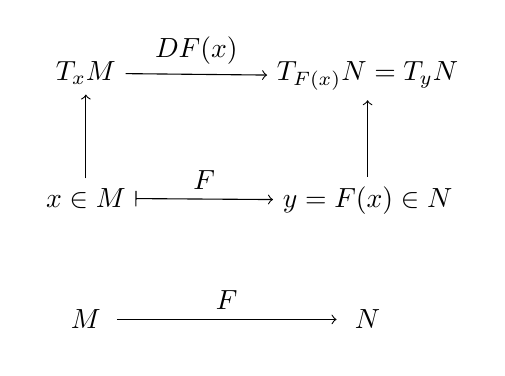
\begin{tikzpicture}
\matrix (m) [matrix of math nodes, row sep=2.8em, column sep=4.8em, minimum width=2.2em]
{
	T_xM & T_{F(x)}N = T_yN \\
	x \in M & y=F(x) \in N  \\ 
	M & N \\ 
};
\path[->]
(m-1-1) edge node [above] {$DF(x)$} (m-1-2)
(m-2-1) edge node [auto] {$$} (m-1-1)
(m-2-2) edge node [auto] {$$} (m-1-2)
(m-3-1) edge node [auto] {$F$} (m-3-2)
;
\path[|->]
(m-2-1) edge node [auto] {$F$} (m-2-2)
;
\end{tikzpicture}   \\
\end{gathered}
\]

Now 
\[
\begin{aligned}
& \text{dim}T_xM = \text{dim}M \\ 
& \text{dim}T_{F(x)}N = \text{dim}N 
\end{aligned}
\]
And 
\[
\text{rank}(DF(x)) \equiv \text{rank of $F$ }
\]
I know that the notation above is confusing, but this is what all Differential Geometry books apparently mean when they say "rank of $F$".  

Now  
\[
\text{rank}(DF(x)) = \text{dim}(\text{im}(DF(x)))  = \text{dim}T_xM \text{ iff } DF(x) \text{ injective }  
\]

If $\forall \, x \in M$, this is the case, then $F$ an \textbf{ immersion }.  

Apply the rank-nullity theorem in this case:  

\[
\begin{gathered}
	\text{rank}(DF(x)) + \text{dim}\text{ker}(DF(x)) = \text{dim}T_xM = \text{dim}M \\ 
	\Longrightarrow \text{rank}(DF(x)) = \text{dim}M \leq \text{dim}T_{F(x)}N = \text{dim}N \text{ or } \text{dim}M \leq \text{dim}N 
\end{gathered}
\]

Now 

\[
\text{rank}(DF(x)) = \text{dim}T_{F(x)}N \text{ iff } DF(x) \text{ surjective }  
\]

If $\forall \, x \in M$, this is the case, then $F$ an \textbf{ submersion }.  

\[
 \text{rank}(DF(x)) = \text{dim}T_{F(x)}N = \text{dim}N  \leq \text{dim}M  
\]

Shastri (2011) has this as the ``Injective Form of Implicit Function Theorem'', Thm. 1.4.5, pp. 23 and Guillemin and Pollack (2010) has this as the ``Local Immersion Theorem'' on pp. 15, Section 3 ``The Inverse Function Theorem and Immersions'' \cite{VGuilleminAPollack2010}.  

\begin{theorem}[Local immersion Theorem i.e. Injective Form of Implicit Function Theorem]\label{Thm:LocalImmersion}
  Suppose $f:M\to N$ immersion at $p$, $q=f(p)$.  

Then $\exists \, $ local coordinates around $p,q$, $x,y$, respectively s.t. $f(x_1\dots x_m) = (x_1 \dots x_m,0 \dots 0)$.  

\end{theorem}

\begin{proof}
  Choose local parametrizations 
\[
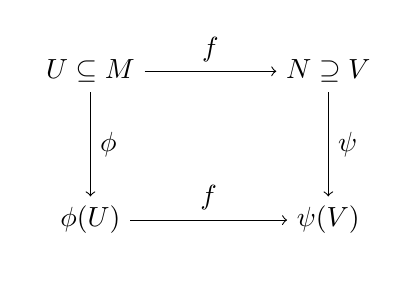
\begin{tikzpicture}
  \matrix (m) [matrix of math nodes, row sep=3.8em, column sep=4.8em, minimum width=2.2em]
  {
    U \subseteq M & N \supseteq V \\
    \phi(U) & \psi(V) \\
};
  \path[->]
  (m-1-1) edge node [above] {$f $} (m-1-2)
          edge node [auto] {$\phi$} (m-2-1)
  (m-1-2) edge node [auto]  {$\psi$} (m-2-2)
  (m-2-1) edge node [auto] {$f$} (m-2-2)
  ;
\end{tikzpicture}  
\quad \quad \, \begin{aligned} & \phi(p) = x \\
  & \psi(q) = y \end{aligned}
\]
$D(\psi f\varphi^{-1}) \equiv Df$.  $Df(p)$ injective (given $f$ immersion).  $Df(p) \in \text{Mat}(n,m)$

By change of basis in $\mathbb{R}^n$, assume $Df(p) = \left( \begin{matrix} I_m \\ 0 \end{matrix} \right)$.  

Now define $\begin{aligned} & \quad \\
  & G : \phi(U) \times \mathbb{R}^{n-m} \to \mathbb{R}^n \\
  & G(x,z) = f(x) + (0,z) \end{aligned}$

Thus, $DG(x,z) =1$ and for open $\phi(U) \times U_2$, $ G(\phi(U)\times U_2)$ open.  

By inverse function theorem, $G$ local diffeomorphism of $\mathbb{R}^n$, at $0$.  

Now $f = G\circ \mathfrak{i}$, where $\mathfrak{i}$ is canonical immersion.  
\[
\begin{gathered}
  G(x,0) = f(x) \\
  \Longrightarrow G^{-1}G(x,0) = (x,0) = G^{-1}f(x)
\end{gathered}
\]

Use $\psi \circ G$ as the local parametrization of $N$ around pt. $q$.  Shrink $U,V$ so that 

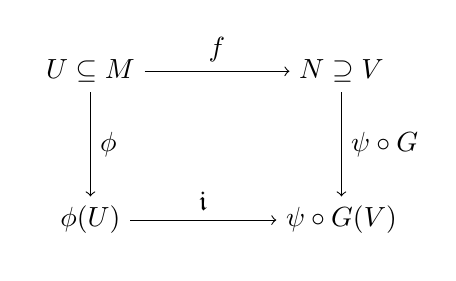
\begin{tikzpicture}
  \matrix (m) [matrix of math nodes, row sep=3.8em, column sep=4.8em, minimum width=2.2em]
  {
    U \subseteq M & N \supseteq V \\
    \phi(U) & \psi\circ G(V) \\
};
  \path[->]
  (m-1-1) edge node [above] {$f $} (m-1-2)
          edge node [auto] {$\phi$} (m-2-1)
  (m-1-2) edge node [auto]  {$\psi\circ G$} (m-2-2)
  (m-2-1) edge node [auto] {$\mathfrak{i}$} (m-2-2)
  ;
\end{tikzpicture}  

\end{proof}






\begin{theorem}[Implicit Function Thm.]
  Let open subset $U\subseteq \mathbb{R}^n \times \mathbb{R}^d$, $(x,y) = (x^1 \dots x^n, y^1 \dots y^k) $ on $U$.  \\
  Suppose smooth $\Phi:U\to \mathbb{R}^k$, $(a,b) \in U$, $c=\Phi(a,b)$

  If $k\times k$ matrix $\frac{ \partial \Phi^i}{ \partial y^j}(a,b)$ nonsingular, then $\exists $ neighborhoods $\begin{aligned} & \quad \\
    & V_0 \subseteq \mathbb{R}^n \text{ of $a$ } \\
    & W_0 \subseteq \mathbb{R}^k \text{ of $b$ } \end{aligned}$ and smooth $F:V_0 \to W_0$ s.t.

  $\Phi^{-1}(c) \bigcap (V_0\times W_0)$ is graph of $F$, i.e. \\
  $\Phi(x,y) =c$ for $(x,y) \in V_0\times W_0$ iff $y=F(x)$.  
  \end{theorem}



\section{Submersions; Rank Theorem} 
cf. pp. 20, Sec. 4 "Submersions", Ch. 1 of Guillemin and Pollack (2010) \cite{VGuilleminAPollack2010}.  

Consider $X,Y\in \text{\textbf{Man}}$, s.t. $\text{dim}X \geq \text{dim}Y$.  

\begin{definition}[submersion] If $f:X\to Y$, \\
if $Df_x \equiv df_x$ is \emph{surjective}, $f\equiv $ \textbf{submersion} at $x$.
\end{definition}
Recall that,  
\[
\begin{gathered}
	Df_x:T_xX \to T_{f(x)}Y \\
	\text{dim}T_xX \geq \text{dim}T_{f(x)}Y
\end{gathered}
\]
\[
\begin{gathered}
\text{rank}Df_x \leq \text{dim}T_{f(x)}Y, \text{ in general, while } \\
\text{rank}Df_x = \text{dim}T_{f(x)}Y \text{ iff } Df_x \text{ surjective }
\end{gathered}
\]

Canonical submersion is standard projection: \\
If $\begin{gathered} \quad \\
\text{dim}X = k \\
\text{dim}Y = l \end{gathered}$, $k\geq l$, 
\[
(a_1 \dots a_k ) \mapsto (a_1 \dots a_l)
\]

\begin{theorem}[Local Submersion Theorem]\label{Thm:LocalSubmersion}
	Suppose $f:X\to Y$ submersion at $x$, and $y = f(x)$, 
	Then $\exists \, $ local coordinates around $x$, $y$ s.t. 
	\[
	f(x_1\dots x_k) = (x_1 \dots x_l)
	\]
	i.e. $f$ locally equivalent to canonical submersion near $x$
\end{theorem}
\begin{proof}
I'll have a side-by-side comparison of my notation and the 1 used in Guillemin and Pollack (2010) \cite{VGuilleminAPollack2010} where I can.	

For charts $(U,\phi), (V,\psi)$ for $X,Y$, respectively, $y=f(x)$ for $x\in X$, 
\[
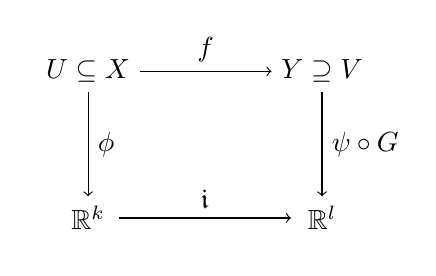
\begin{tikzpicture}
\matrix (m) [matrix of math nodes, row sep=3.8em, column sep=4.8em, minimum width=2.2em]
{
	U \subseteq X & Y \supseteq V \\
	\mathbb{R}^k &  \mathbb{R}^l \\
};
\path[->]
(m-1-1) edge node [above] {$f $} (m-1-2)
edge node [auto] {$\phi$} (m-2-1)
(m-1-2) edge node [auto]  {$\psi\circ G$} (m-2-2)
(m-2-1) edge node [auto] {$\mathfrak{i}$} (m-2-2)
;
\end{tikzpicture} \quad \quad \, 
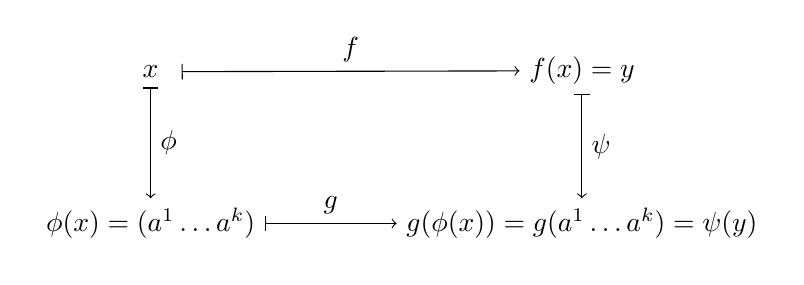
\begin{tikzpicture}
\matrix (m) [matrix of math nodes, row sep=3.8em, column sep=4.8em, minimum width=2.2em]
{
	 x & f(x)=y \\
	\phi(x)=(a^1\dots a^k) &  g(\phi(x))=g(a^1\dots a^k)=\psi(y) \\
};
\path[|->]
(m-1-1) edge node [above] {$f $} (m-1-2)
edge node [auto] {$\phi$} (m-2-1)
(m-1-2) edge node [auto]  {$\psi$} (m-2-2)
(m-2-1) edge node [auto] {$g$} (m-2-2)
;
\end{tikzpicture}
\]
$Dg_x$ surjective, so assume it's a $l\times k$ matrix $\left[ \begin{matrix} \mathbf{1}_l & 0 \end{matrix} \right]$.  

Define
\begin{equation}
\begin{aligned}
& G:U \subset \mathbb{R}^k \to \mathbb{R}^k  \\
& G(a)\equiv G(a^1\dots a^k) := (g(a), a_{l+1}, \dots , a_k)
\end{aligned}
\end{equation}
Now
\begin{equation}
DG(a)  = \left[ \begin{matrix} \mathbf{1}_l & 0 \\ & \mathbf{1}_{k-l} \end{matrix} \right] = \mathbf{1}_k
\end{equation}
so $G$ local diffeomorphism (at $0$).  

So $\exists \, $ $G^{-1}$ as local diffeomorphism of some $U'$ of $a$ into $U\subset \mathbb{R}^k$.  

By construction, 
\begin{equation}
g=\mathbb{P}_l \circ G
\end{equation}
where $\mathbb{P}_l$ is the \emph{canonical submersion}, the projection operator onto $\mathbb{R}^l$.  
\[
g\circ G^{-1} = \mathbb{P}_l
\]
(since $G$ diffeomorphism)

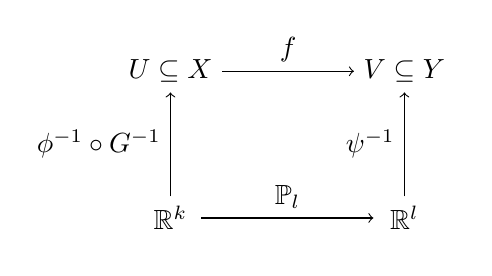
\begin{tikzpicture}
\matrix (m) [matrix of math nodes, row sep=3.8em, column sep=4.8em, minimum width=2.2em]
{
	U\subseteq X &  V\subseteq Y \\
	\mathbb{R}^k &  \mathbb{R}^l \\
};
\path[->]
(m-2-1) edge node [auto] {$\phi^{-1}\circ G^{-1}  $} (m-1-1)
edge node [auto] {$\mathbb{P}_l$} (m-2-2)
(m-1-1) edge node [auto]  {$f$} (m-1-2)
(m-2-2) edge node [auto] {$\psi^{-1}$} (m-1-2)
;
\end{tikzpicture}
for \\
$\Longrightarrow $ 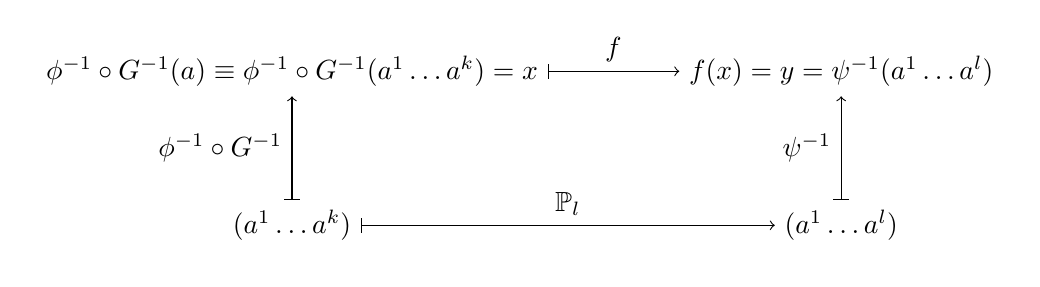
\begin{tikzpicture}
\matrix (m) [matrix of math nodes, row sep=3.8em, column sep=4.8em, minimum width=2.2em]
{
	\phi^{-1}\circ G^{-1}(a)\equiv \phi^{-1}\circ G^{-1}(a^1\dots a^k)=x & f(x)=y=\psi^{-1}(a^1\dots a^l) \\
	(a^1\dots a^k) &  (a^1\dots a^l) \\
};
\path[|->]
(m-2-1) edge node [auto] {$\phi^{-1}\circ G^{-1}  $} (m-1-1)
edge node [auto] {$\mathbb{P}_l$} (m-2-2)
(m-1-1) edge node [auto]  {$f$} (m-1-2)
(m-2-2) edge node [auto] {$\psi^{-1}$} (m-1-2)
;
\end{tikzpicture}


	\end{proof}
"An obvious corollary worth noting is that if $f$ is a submersion at $x$, then it is actually a submersion in a whole neighborhood of $x$." Guillemin and Pollack (2010) \cite{VGuilleminAPollack2010}

Suppose $f$ submersion at $x\in f^{-1}(y)$.  

By local submersion theorem
\[
f(x_1\dots x_k)=(x_1 \dots x_l)
\]
Choose $y=(0, \dots , 0)$. 

Then, near $x$, $f^{-1}(y) = \lbrace (0, \dots 0 , x_{l+1} \dots x_k)\rbrace$ i.e. let $V\ni x$ neighborhood of $x$, define $(x_1 \dots x_k)$ on $V$.  

Then $f^{-1}(y) \bigcap V = \lbrace (0\dots 0 , x_{l+1} , \dots x_k) | x_1 = 0 , \dots x_l = 0\rbrace$.

Thus $x_{l+1}, \dots x_k$ form a coordinate system on open set $f^{-1}(y) \bigcap V \subseteq f^{-1}(y)$.  

Indeed, 
\[
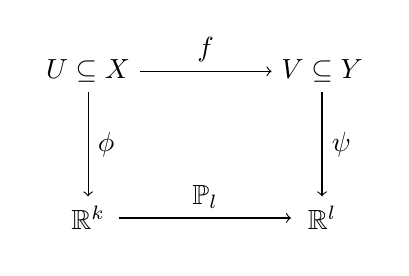
\begin{tikzpicture}
\matrix (m) [matrix of math nodes, row sep=3.8em, column sep=4.8em, minimum width=2.2em]
{
	U \subseteq X &  V\subseteq Y \\
	\mathbb{R}^k &  \mathbb{R}^l \\
};
\path[->]
(m-1-1) edge node [auto] {$ f  $} (m-1-2)
edge node [auto] {$ \phi $} (m-2-1)
(m-2-1) edge node [auto]  {$\mathbb{P}_l$} (m-2-2)
(m-1-2) edge node [auto] {$\psi$} (m-2-2)
;
\end{tikzpicture} \qquad \, 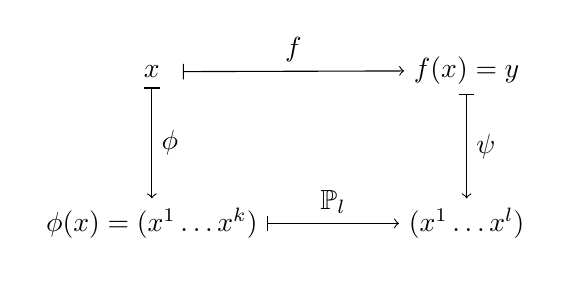
\begin{tikzpicture}
\matrix (m) [matrix of math nodes, row sep=3.8em, column sep=4.8em, minimum width=2.2em]
{
	x &  f(x)=y \\
	\phi(x)=(x^1\dots x^k) &  (x^1\dots x^l) \\
};
\path[|->]
(m-1-1) edge node [auto] {$ f  $} (m-1-2)
edge node [auto] {$ \phi $} (m-2-1)
(m-2-1) edge node [auto]  {$\mathbb{P}_l$} (m-2-2)
(m-1-2) edge node [auto] {$\psi$} (m-2-2)
;
\end{tikzpicture} 
\]
and now 
\[
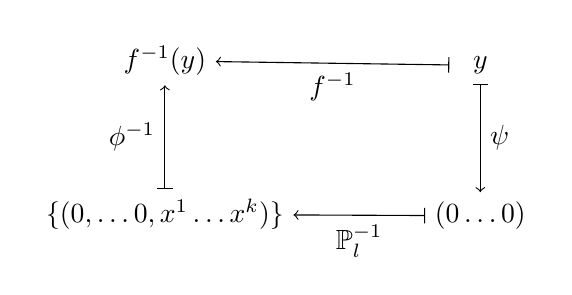
\begin{tikzpicture}
\matrix (m) [matrix of math nodes, row sep=3.8em, column sep=4.8em, minimum width=2.2em]
{
	f^{-1}(y) &  y \\
	\lbrace (0, \dots 0,x^1\dots x^k) \rbrace &  (0\dots 0) \\
};
\path[|->]
(m-1-2) edge node [auto] {$ f^{-1}  $} (m-1-1)
edge node [auto] {$ \psi $} (m-2-2)
(m-2-2) edge node [auto]  {$\mathbb{P}_l^{-1}$} (m-2-1)
(m-2-1) edge node [auto] {$\phi^{-1}$} (m-1-1)
;
\end{tikzpicture} 
\]

\subsection{Rank Theorem}

Lee (2012) \cite{JLee2012} in pp. 85, Ch. 4 Submersions, Immersions, and Embeddings, combines Theorems \ref{Thm:LocalImmersion}, \ref{Thm:LocalSubmersion} (local immersion and local submersion theorems, respectively) into the "Rank Theorem" (cf. Thm 4.12 "Rank Theorem" of Lee (2012)):

\begin{theorem}[Rank Theorem]
Suppose smooth manifolds $M, N$, $\text{dim}{M} = m$, $\text{dim}{N} = n$, smooth map $F:M \to N$, $F$ has constant rank $r$. \\
$\forall \, p \in M$, $\exists \, $ smooth charts $(U, \varphi)$ for $M$, centered at $p$, $(V, \psi)$ for $N$, centered at $F(p)$, s.t. 
\[
F(U) \subseteq V
\]
in which $F$ has coordinate representation of form
\begin{equation}
\widehat{F}(x^1 \dots x^r, x^{r+1} \dots x^m) = (x^1 \dots x^r , 0 \dots 0)
\end{equation}

Particularly, if $F$ smooth submersion,
\[
\widehat{F}(x^1 \dots x^n, x^{n+1} \dots x^m) = (x^1 \dots x^n)
\]

and if $F$ smooth immersion

\[
\widehat{F}(x^1 \dots x^m ) = (x^1 \dots x^m , 0 \dots 0)
\]
\end{theorem}

\[
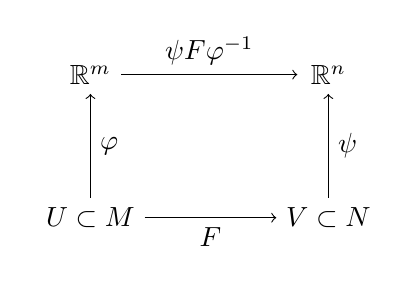
\begin{tikzpicture}
\matrix (m) [matrix of math nodes, row sep=3.8em, column sep=4.8em, minimum width=2.2em]
{
	\mathbb{R}^m &  \mathbb{R}^n \\
	U \subset M &  V \subset N \\
};
\path[->]
(m-1-1) edge node [above] {$ \psi F \varphi^{-1} $} (m-1-2)
(m-2-1) edge node [right] {$\varphi$} (m-1-1)
(m-2-1) edge node [below] {$F$} (m-2-2)
(m-2-2) edge node [right] {$\psi$} (m-1-2)
;
\end{tikzpicture}
\]
Also remember that $DF(p) : T_p M \to T_{F(p)}N$
\begin{proof}
	$DF(p)$ has rank $r$ (given). Then $DF(p)$ is some $r\times r$ submatrix of a $n\times m$ matrix s.t. $\text{det}DF(p)$ nonzero. 
	
	By change of basis in $\mathbb{R}^n$, or reordering coordinates, assume $DF(p)$ is upper left submatrix $\left( \frac{ \partial F^i}{ \partial x^j} \right) \quad \, \forall \, i,j = 1, \dots r$. 
	
	Relabel standard coordinate as 
	\[
	\begin{aligned} 
		& (x,y) = (x^1 \dots x^r, y^1 \dots y^{m-r})\in \mathbb{R}^m \\
		& (v,w) = (v^1 \dots v^r, w^1 \dots w^{n-r}) \in \mathbb{R}^n 
	\end{aligned}
	\]
	By initial translations of coordinates, assume without loss of generality $p = (0, 0)$, $F(p) = (0,0)$
	
	Suppose 
	\[
	F(x,y) = (Q(x,y) , R(x,y)) 
	\]
	for some smooth maps $Q : U\to \mathbb{R}^r$, $R:U\to \mathbb{R}^{n-r}$

	Define
	\[
	\begin{aligned}
	& \varphi : U \to \mathbb{R}^m \\ 
	& \varphi(x,y) = (Q(x,y), y)
	\end{aligned}
	\]
	so 
	\[
	D\varphi(0,0) = \left( \begin{matrix} \frac{ \partial Q^i }{ \partial x^j} (0,0) & \frac{ \partial Q^i }{ \partial y^j}(0,0) \\ 0 & \delta^i_j \end{matrix} \right) 
	\]
	$D\varphi(0,0)$ nonsingular, since $\text{det}\frac{\partial Q^i }{ \partial x^j} \neq 0$ (by hypothesis).
	
	By inverse function thm., $\exists \, $ connected neighborhoods $U_0$ of $(0,0)$, $\widetilde{U}_0$ of $\varphi(0,0) = (0,0)$ s.t. 
	\[
	\varphi : U_0 \to \widetilde{U}_0
	\]
	is a diffeomorphism.
	
	By shrinking $U_0, \widetilde{U}_0$, assume $\widetilde{U}_0$ open cube.
	
	Write $\varphi^{-1}(x,y) = (A(x,y), B(x,y))$, for some smooth functions $\begin{aligned} & \quad \\ 
	& A:\widetilde{U}_0 \to \mathbb{R}^r \\ 
	& B: \widetilde{U}_0 \to \mathbb{R}^{m-r}\end{aligned}$,
	\[
	(x,y) = \varphi(A(x,y) , B(x,y)) = (Q(A(x,y), B(x,y)), B(x,y))
	\]
	\[
	\Longrightarrow \begin{aligned} & B(x,y) = y \\ 
	& \varphi^{-1}(x,y) = (A(x,y), y) \end{aligned}  
	\]
	
	\[
	\varphi \varphi^{-1} = 1 \Longrightarrow x = Q(A(x,y), y)
	\]
	
	Recall that we had hypotehsized that 
	\[
	F(x,y) = (Q(x,y) , R(x,y))
	\]
	Then
	\[
	\begin{gathered}
		F \circ \varphi^{-1}(x,y) = F(A(x,y), y) = (Q(A(x,y), y), R(A(x,y), y)) = (x, R(A(x,y), y))
	\end{gathered}
	\]

	and so 
	\[
	F\circ \varphi^{-1}(x,y) = (x, \widetilde{R}(x,y))
	\]
	where $\begin{aligned} & \quad \\ 
	& \widetilde{R} : \widetilde{U}_0 \to \mathbb{R}^{n-r} \\
	& \widetilde{R}(x,y) = R(A(x,y), y)
	\end{aligned}$

	Compute
	\[
	\begin{gathered}
		D(F\circ \varphi^{-1})(x,y) = \left( \begin{matrix} \delta^i_j & 0 \\
		\frac{ \partial \widetilde{R}^i }{ \partial x^j}(x,y) & \frac{ \partial \widetilde{R}^i }{ \partial y^j}(x,y) \end{matrix} \right) 	
	\end{gathered}
	\]
	
	Since composing with a diffeomorphism doesn't change rank of map, $D(F\circ \varphi^{-1})$ has rank $r$ everywhere in $\widetilde{U}_0$.  

	$\left( \begin{matrix} \delta^i_j \\ \frac{ \partial \widetilde{R}^i }{ \partial x^j}(x,y) \end{matrix} \right)$ $j=1\dots r$ are linearly independent, so $\frac{\partial \widetilde{R}^i}{ \partial y^j}(x,y) = 0$ on $\widetilde{U}_0$, so $\widetilde{R}^i$ independent of $y^j$.
	
	Let $S(x) = \widetilde{R}(x,0)$, then
	\[
	F \circ \varphi^{-1}(x,y) = (x, S(x))
	\]
	Let open $V_0 \subseteq V$, $(0,0) \in V$ be an open subset $V_0 = \lbrace (v,w) \in V: (v,0) \in \widetilde{U}_0 \rbrace$. \\
	Then $V_0 $ is a neighborhood of $(0,0)$.
	
	Because $\widetilde{U}_0$ is a cube, $F \circ \varphi^{-1}(x,y) = (x, S(x))$,
	\[
	F\circ \varphi^{-1}(\widetilde{U}_0) \subseteq V_0
	\]
	so $F(U_0) \subseteq V_0$.
	
	Define $\begin{aligned} & \quad \\ 
	& \psi : V_0 \to \mathbb{R}^n \\
	& \psi (v,w) = (v, w- S(v)) \end{aligned}$
	
	Because $\psi^{-1}(s,t) = (s, t+S(s))$, \\
	it is a diffeomorphism.
	
	Thus $(V_0, \psi)$ is a smooth chart. 
	
	\[
	\psi \circ F (\varphi^{-1}(x,y)) = \psi(x, S(x)) = (x, S(x) - S(x)) = (x, 0)
	\]
	

	\end{proof}


\begin{definition}[regular value]
	For smooth $f:X\to Y$, $X,Y \in \text{\textbf{Man}}$, \\
	$y\in Y$ is a \textbf{regular value} for $f$ if $Df_x:T_xX \to T_y Y$ surjective $\forall \, x$ s.t. $f(x)=y$.  
	
	$y\in Y$ \textbf{critical value} if $y$ not a regular value of $f$.  
\end{definition}

Absil, Mahony, and Sepulchre \cite{AMS2008} pointed out that another definition for a \emph{regular value} can utilize the theorem that $\text{rank}$ of $Df \equiv DF = \text{dim} T_pN = \text{dim} N$, iff $DF(p)$ surjective, for $p\in M$, $F:M\to N$.  Then 

\textbf{regular value} $y \in N$, of $F$, if rank of $F \equiv \text{rank}(DF(x)) = \text{dim}N$, $\forall \, x \in F^{-1}(y)$, for $F:M\to N$.  


\begin{theorem}[Preimage theorem]
If $y$ regular value of $f:X\to Y$, \\
$f^{-1}(y)$ is a submanifold of $X$, with $\text{dim}f^{-1}(y)=\text{dim}X - \text{dim}Y$
\end{theorem}
\begin{proof}
Given $y$ is a regular value of $f:X\to Y$,  \\
$\forall \, x \in f^{-1}(y)$, $Df_x:T_xX \to T_yY$ is surjective.  By local submersion theorem, 
\[
f(x^1 \dots x^k) = (x^1 \dots x^l)=y
\]	
Since $x\in f^{-1}(y)$, $(x^1\dots x^k)=(y^1 \dots y^l,x^{l+1}\dots x^k)$.  

For this chart for $(U,\varphi)$, $U\ni x$, consider $(U\cap f^{-1}(y),\psi)$ with $\psi(x) = (x^{l+1}\dots x^k) \quad \, \forall \, x\in U\cap f^{-1}(y)$.  

$\forall \, f^{-1}(y)$ submanifold with $\text{dim}f^{-1}(y) = k-l = \text{dim}X-\text{dim}Y$.  
	\end{proof}

\emph{Examples for emphasis}

If $\text{dim}X > \text{dim}Y$, \\
\phantom{\qquad \, } if $y\in Y$, regular value of $f:X\to Y$, \\
\phantom{\qquad \, \qquad \, } $f$ submersion, $\forall \, x \in f^{-1}(y)$ \\
If $\text{dim}X = \text{dim}Y$, \\
\phantom{\qquad \, } $f$ local diffeomorphism $\forall \, x\in f^{-1}(y)$ \\
If $\text{dim}X < \text{dim}Y$, $\forall \, y\in f(X)$ is a critical value.  


\textbf{Example: $O(n)$ as a submanifold of $\text{Mat}(n,n)$}

Given $\text{Mat}(n,n)\equiv M(n) = \lbrace n \times n \text{ matrices } \rbrace$ is a manifold; in fact $\text{Mat}(n,n) \cong \mathbb{R}^{n^2}$, \\
Consider $O(n) = \lbrace A \in \text{Mat}(n,n) | AA^T = 1\rbrace$.  
\begin{equation}
AA^T \in \text{Sym}(n) \equiv S(n) = \lbrace S\in \text{Mat}(n,n) | S^T = S \rbrace = \lbrace \text{ symmetric $n\times n$ matrices } \rbrace
\end{equation}
$\text{Sym}(n)$ submanifold of $\text{Mat}(n,n)$, $\text{Sym}(n)$ diffeomorphic to $\mathbb{R}^k$ (i.e. $\text{Sym}(n) \cong \mathbb{R}^k$), $k:= \frac{n (n+1)}{2}$.  

\[
\begin{aligned}
	& f:\text{Mat}(n,n) \to \text{Sym}(n) \\
	& f(A) = AA^T
\end{aligned}
\]
Notice $f$ is smooth, 
\[
\begin{gathered}
f^{-1}(1) = O(n) \\
Df_A(B) = \lim_{s\to 0} \frac{ f(A+sB) - f(A) }{s} = \lim_{s\to 0} \frac{(A+sB)(A^T + sB^T)- AA^T}{s} = AB^T +BA^T
\end{gathered}
\]
If $Df_A : T_A\text{Mat}(n,n) \to T_{f(A)}\text{Sym}(n)$ surjective when $A\in f^{-1}(1) = O(n)$ (???).  





\begin{proposition} If smooth $g_1\dots g_l \in C^{\infty}(X)$ on $X$ are independent $\forall \, x\in X$, s.t. $g_i(x)=0$, $\forall \, i = 1\dots l$, \\
	then $Z=\lbrace x\in X | g_1(x) = \dots = g_l(x)=0 \rbrace = $ set of "common zeros" is a \emph{submanifold} of $X$ s.t. $\text{dim}Z = \text{dim}X- l$.  
	
	Take \emph{note} that $g_1 \dots g_l$ are independent at $x$ means, really, that $D(g_1)_x \dots D(g_l)_x$ are linearly independent on $T_xX$.  
\end{proposition}
\begin{proof}
Suppose smooth $g_1 \dots g_l \in C^{\infty}(X)$ on manifold $X$ s.t. $\text{dim}X = k\geq l$.  

Consider $g=(g_1\dots g_l):X \to \mathbb{R}^l$, $Z\equiv g^{-1}(0)$.  

Since $\forall \, g_i$ smooth, $D(g_i)_x:T_xX \to \mathbb{R}$ linear.  

Now for 
\[
Dg_x = (D(g_1)_x \dots D(g_l)_x):T_xX \to \mathbb{R}^l
\]	
By rank-nullity theorem (linear algebra), $Dg_x$ surjective iff $\text{rank}Dg_x = l$ i.e. $l$ functionals $D(g_1)_x \dots D(g_l)_x$ are linearly independent on $T_xX$.  

"We express this condition by saying the $l$ functions $g_1\dots g_l$ are independent at $x$."  (Guillemin and Pollack (2010) \cite{VGuilleminAPollack2010})  
	
	
	\end{proof}

\section{Submanifolds; immersed submanifold, embedded submanifolds, regular submanifolds}  

\begin{definition}[Embedded Submanifold]
	
\end{definition}

Recall immersion:  \\
$F:M \to N$ immersion iff $DF$ injective, i.e. iff $\text{rank}DF = \text{dim}M$.  

Consider manifolds $M\subseteq N$.  \\
Consider inclusion map $\begin{aligned} & \quad \\ 
	& i:M\to N \\
	& i: x \mapsto x \end{aligned}$.  
	
	If $i$ immersion, $Di(x) = \frac{\partial y^i}{ \partial x^j} = \delta_j^{\  \  i}$ if $y^i = x^i$, $\forall \, i =1,\dots \text{dim}M$.  
	
\begin{definition}[immersed submanifold]
	\textbf{immersed submanifold} $M \subseteq N$ if inclusion $i:M\to N$ is an immersion.  
\end{definition}	
cf. 3.3 Embedded Submanifolds of Absil, Mahony, and Sepulchre \cite{AMS2008}, also Ch. 5 Submanifolds, pp. 108, \textbf{Immersed Submanifolds} of  John Lee (2012) \cite{JLee2012}.  

Immersed submanifolds often arise as images of immersions.  

\begin{proposition}[Images of Immersions as submanifolds]
	Suppose smooth manifold $M$, \\
	\phantom{Suppose } smooth manifold with or without boundaries $N$, \\
	injective, smooth immersion $F:M\to N$ ($F$ injective itself, not just immersion)  
	
Let $S=F(M)$.  

Then $S$ has unique topology and smooth structure of smooth submanifolds of $N$ s.t. $F:M\to S$ diffeomorphism.  
	
\end{proposition}
cf. Prop. 5.18 of John Lee (2012) \cite{JLee2012}.  

\begin{proof}
Define topology of $S$: set $U\subseteq S$ open iff $F^{-1}(U) \subseteq M$ open ($F^{-1}(U\cap V) = F^{-1}(U) \cap F^{-1}(V), F^{-1}(U\cup V) =F^{-1}(U) \cup F^{-1}(V)$).  \\
Define smooth structure of $S$: $\lbrace F(U), \varphi \circ F^{-1}  | (U,\varphi) \in \text{atlas for $M$, i.e. $(U,\varphi)$ any smooth chart of $M$}\rbrace$.  

"smooth compatibility condition": 
\[
(\varphi_2\circ F^{-1}) (\varphi_i F^{-1})^{-1} = \varphi_2 \circ F^{-1}F\varphi_1^{-1} = \varphi_2 \varphi_1^{-1}
\]
since $\varphi_2\varphi_1^{-1}$ diffeomorphism ($\varphi_2 \varphi_1^{-1}$ bijection and it and inverse is differentiable) 

$F$ diffeomorphism onto $F(M)$.  

	and these are the only topology and smooth structure on $S$ with this property: 
	\[
	S \xrightarrow{F^{-1}} M \xrightarrow{F} N \qquad \, = \qquad \, S \hookrightarrow M
	\]
	and $F^{-1}$ diffeomorphism, $F$ smooth immersion, so $i : S \to M$ smooth immersion.  
	\end{proof}

	










\section{Tensors}

I'll go through Ch.7 \emph{Tensors} of Jeffrey Lee (2009) \cite{JLee2009}.  

\begin{definition}[7.1\cite{JLee2009}] Let $V,W$ be modules over commutative ring $R$, with unity.  

Then, algebraic $W$-valued tensor on $V$ is multilinear map.  
\begin{equation}
	\tau: V_1 \times V_2 \times \dots \times V_m \to W
\end{equation}
where $V_i = \lbrace V,V^* \rbrace$ \quad \, $ \forall \, i=1,2,\dots m$.  

If for $r,s$ s.t. $r+s =m$, there are $r$ \, $V_i = V^*$, $s \, V_i = V$, tensor is $r$-contravariant, $s$-covariant; also say tensor of total type $\binom{r}{s}$.  
\end{definition}

EY : 20170404 Note that 
\[
\begin{aligned}
	& ( \tau_{\beta}^{i\alpha} \frac{ \partial }{ \partial x^i } \text{ or } \tau_{\beta}^{i\alpha} e_i )(\omega_j dx^j \text{ or } \omega_je^j  \in V^*) \\ 
	& ( \tau^{\beta}_{i\alpha} dx^i \text{ or } \tau^{\beta}_{i\alpha} e^i )( X^j \frac{ \partial }{ \partial x^j} \text{ or } X^j e_j  \in V) 
\end{aligned}
\]

$\exists \,$ natural map $\begin{aligned} & \quad \\ 
	& V\to V^{**} \\ 
& v \mapsto \widetilde{v} \end{aligned}$,  $\begin{aligned} & \quad \\ 
	& \widetilde{v} : \alpha \mapsto \alpha(v) \end{aligned}$.  If this map is an isomorphism, $V$ is \textbf{reflexive} module, and identify $V$ with $V^{**}$.  

\exercisehead{7.5} Given vector bundle $\pi: E \to M$, open $U\subset M$, consider sections of $\pi$ on $U$, i.e. cont. $s:U\to E$, where $(\pi\circ s)(u)=u$, \, $\forall \, u \in U$.  

Consider $E^* \ni \omega =\omega_i e^i$.  

$\forall \, s\in \Gamma(E)$, $\omega(s) = \omega_i(s(x))^i$, \, $\forall \, x \in U\subset M$.  So define $\widetilde{s}: \omega,x\mapsto \omega(s(x))$, \, $\forall \, x \in U$.  

If $\widetilde{s} =0$, $\widetilde{s}(\omega,x) = \omega(s(x)) =0$ \quad \, $\forall \, \omega \in E^*$, $\forall \, x\in U$, and so $s=0$.  (Let $\omega_i = \delta_{iJ}$ for some $J$, and so $s^J(x) =0$ \quad \, $\forall \, J$).  

$s=0$.  So $\text{ker}(s\mapsto \widetilde{s}) = \lbrace 0 \rbrace$ (so condition for injectivity is fulfilled).  

Since $\widetilde{s}:\omega,x\mapsto \omega(s(x))$, $\forall \, \omega \in E^*$, $\forall \, x \in U$, $s\mapsto \widetilde{s}$ is surjective.  

$s\mapsto \widetilde{s}$ is an isomorphism so $\Gamma(E)$ is a \emph{reflexive} module.  


\begin{proposition}
For $R$ a ring (special case), $\exists \, $ module homomorphism:  \\

tensor product space $\to $ tensor, as a multilinear map, i.e. $\exists$ \,  
\begin{equation}
\begin{aligned}
&	\left( \otimes_{i=1}^r V \right) \otimes \left( \otimes_{j=1}^s V^* \right) \to T^r_{ \, \, s}(V;R)   \\
& u_1 \otimes \dots \otimes u_r \otimes \beta^1 \otimes \dots \otimes \beta^s \in \left( \otimes^r V \right) \otimes \left( \otimes^s V^* \right) \mapsto (\alpha^1 \dots \alpha^r, v_1 \dots v_s) \mapsto \alpha^1(u_1) \dots \alpha^r(u_r) \beta^1(v_1) \dots \beta^s(v_s)  
\end{aligned}
\end{equation}
\end{proposition}

Indeed, consider 
\[
(\alpha^1 \dots \alpha^r, v_1 \dots v_s) \in \underbrace{V^* \times \dots \times V^* }_{r} \times \underbrace{ V\times \dots \times V}_{s} \mapsto \alpha^1(u_1) \dots \alpha^r(u_r) \beta^1(v_1) \dots \beta^s(v_s)
\]
and so for 
\[
\begin{aligned}
	& \alpha^i = \alpha^i_{\mu} e^{\mu} , \, & \, i =1,2, \dots r, \, & \, \mu = 1,2, \dots \text{dim}V^* \\ 
	& v_i = v_i^{\mu} e_{\mu} , \, & \, i = 1,2, \dots s, \, & \, \mu = 1, 2, \dots \text{dim}V 
\end{aligned} \qquad \, \begin{aligned}
& \alpha^i(u_i) = \alpha^i_{\mu} u^{\mu}_i \\ 
 & \beta^i(v_i) = \beta^i_{\mu} v^{\mu}_i
\end{aligned}
\]
So that 
\[
\begin{gathered}
	\alpha^1(u_1) \dots \alpha^r(u_r) \beta^1(v_1) \dots \beta^s(v_s) = \alpha^1_{\alpha_1}u^{\alpha_1}_1 \dots \alpha^r_{\alpha_r} u^{\alpha_r}_r \beta^1_{\mu_1} v^{\mu_1}_1 \dots \beta^s_{\mu_s} v^{\mu_s}_s = \\
	= (u^{\alpha_1}_1 \dots u_r^{\alpha_r} \beta^1_{\mu_1} \dots \beta^s_{\mu_s})(\alpha^1_{\alpha_1} \dots \alpha^r_{\alpha_r} v_1^{\mu_1} \dots v_s^{\mu_s} )
\end{gathered}
\]
Identify $u_1 \otimes \dots \otimes u_r \otimes \beta^1 \otimes \dots \otimes \beta^s$ with this multiplinear map.  

\begin{proposition}
If $V$ is finite-dim. vector space, or if $V=\Gamma(E)$, for vector bundle $E\to M$, map
\begin{equation}
\left( \otimes_{i=1}^r V \right)  \otimes \left( \otimes_{j=1}^s V^* \right) \to T^r_{ \, \, s}(V;R)
\end{equation}
is an isomorphism.  
\end{proposition}

\begin{definition}
tensor that can be written as 
\begin{equation}
u_1\otimes \dots \otimes u_r \otimes \beta^1 \otimes \dots \otimes \beta^s \equiv u_1\otimes \dots \otimes \beta^s 
\end{equation}
is \textbf{simple} or \textbf{decomposable}.  
\end{definition}
Now well that not \emph{all} tensors are simple.  

\begin{definition}[7.7\cite{JLee2009}, tensor product]
$\forall \, S\in T^{r_1}_{ \,\, s_1}(V)$, $\forall \, T \in T^{r_2}_{ \,\, s_2}(V)$, \\
define tensor product 
\begin{equation}
\begin{gathered}
S\otimes T\in T^{r_1+r_2}_{ \, \, \, s_1+s_2}(V) \\
	S\otimes T( \theta^1\dots \theta^{r_1 + r_2}, v_1 \dots v_{s_1+s_2}) := S(\theta^1\dots \theta^{r_1}, v_1\dots v_{s_1})T(\theta^{r_1+1}\dots \theta^{r_1+r_2}, v_{s_1+1}\dots v_{s_1 + s_2} )
\end{gathered}
\end{equation}
\end{definition}

\begin{proposition}[7.8\cite{JLee2009}]
\end{proposition}







\[
\begin{gathered}
	\tau^{ i_1 \dots i_r }_{ \phantom{i_1 \dots i_r} j_1 \dots j_s} e_{i_1} \otimes \dots \otimes e_{i_r} \otimes e^{j_1}\otimes \dots \otimes e^{j_s} = \tau(e^{i_1} \dots e^{i_r}, e_{j_1} \dots e_{j_s} )e_{i_1} \otimes \dots \otimes e_{i_r} \otimes e^{j_1} \otimes \dots \otimes e^{j_s} = \tau 
\end{gathered}
\]
So $\lbrace e_{i_1}\otimes \dots \otimes e_{i_r} \otimes e^{j_1} \otimes \dots \otimes e^{j_s} | i_1 \dots i_{r}, j_1\dots j_s \in 1 \dots n \rbrace$ spans $T^r_{\,\, s}(V;R)$

\exercisehead{7.11}  Let basis for $V$ \, $e_1 \dots e_n$, corresponding dual basis for $V^*$ \,  $e^1 \dots e^n$ \\ 
Let basis for $V$ \, $\overline{e}_1 \dots \overline{e}_n$, corresponding dual basis for $V^*$ \,  $\overline{e}^1 \dots \overline{e}^n$ \\
s.t. 
\[
\begin{aligned}
	& \overline{e}_i = C^k_{ \,\, i} e_k \\
	& \overline{e}^i = (C^{-1})^i_{ \, \, k} e^k
\end{aligned}
\]
EY:20170404, keep in mind that
 
\[
\begin{aligned}
	&	Ax = e_i A^i_{ \, \, k} e^k(x^j e_j) = e_i A^i_{ \,\,j} x^j = A^i_{ \, \, j} x^j e_i \\ 
 & Ae_j = e_k A^k_{ \, \, i} e^i (e_j) = A^k_{ \,\, j} e_k = \overline{e}_j
\end{aligned}
\]
\[
\begin{gathered}
\overline{\tau}^i_{ \,\, jk} \overline{e}_i \otimes \overline{e}^j \otimes \overline{e}^k = \overline{\tau}^i_{ \, \, jk} C^l_{ \, \, i} e_l (C^{-1})^j_{ \,\, m} e^m(C^{-1})^k_{ \, \, n} e^n = \overline{\tau}^i_{ \, \, jk} C^l_{ \, \, i } (C^{-1})^j_{ \,\, m} (C^{-1})^k_{ \,\, n} = \tau^l_{ \,\, mn}   \\
\overline{\tau}^i_{ \,\, jk} = C^c_{ \,\, k} C^b_{ \,\, j} (C^{-1})^i_{ \,\, a} \tau^a_{\,\, bc}
\end{gathered}
\]



On Remark 7.13 of Jeffrey Lee (2009) \cite{JLee2009}:  first, egregious typo for $L(V,V)$; it shoudl be $L(V,W)$.  Onward, \\
for $L(V,W)$, \\
consider $W\otimes V^* \ni w\otimes \alpha$ s.t.
\[
(w\otimes \alpha)(v) = \alpha(v)w\in W, \, \forall \, v\in V, \text{ so } w\otimes \alpha \in L(V,W)
\]

Now consider (category of) left $R$-module, 
\begin{equation}
{\,}_R\textbf{Mod} \ni {\,}_{\text{Mat}_{\mathbb{K}}(N,M) } \mathbb{K}^N
\end{equation}
where
\[
\begin{aligned}
	& V=\mathbb{K}^N \\ 
&	  W = \mathbb{K}^M
\end{aligned}
\]
For $A\in \text{Mat}_{\mathbb{K}}(N,M)$, $x\in \mathbb{K}^N$, 
\[
e_i A^i_{ \,\ , \mu} e^{\mu}(x^{\nu} e_{\nu}) = Ax = e_iA^i_{\,\, \mu} x^{\mu} , \quad \, i=1,2,\dots M, \, \mu = 1,2, \dots N
\]
\[
A\in \text{Mat}_{\mathbb{K}}(N,M) \cong W\otimes V^* \cong L(V,W)
\]
Consider 
\[
\begin{aligned}
	& \alpha \in (\mathbb{K}^N)^* = V^* \\
	& w\in \mathbb{K}^M = W
\end{aligned} \qquad \, \begin{aligned}
	& \alpha = \alpha_{\mu} e^{\mu} \\ 
	& w=w^ie_i
\end{aligned}
\]
\[
\alpha \otimes w = w \otimes \alpha = w^i\alpha_{\mu} e_i \otimes e^{\mu}
\]
(remember, isomoprhism between $\text{Mat}_{\mathbb{K}}(N,M)$ and $W\otimes V^*$ guaranteed, if $V,W$ are free $R$-modules, $R=\mathbb{K}$).

Let $V,W$ be left $R$-modules, i.e. $V,W \in {\,}_R\text{\textbf{Mod}}$.  
\[
V^* \in \text{\textbf{Mod}}_R
\]
For $V^*\otimes W \in \text{\textbf{Mod}}_R\otimes {\,}_R\text{\textbf{Mod}}$  
\[
\alpha \in V^*, w\in W
\]
\[
(\alpha \otimes w)(v) = \alpha(v)w, \text{ for } v\in V \in {\,}_R\text{\textbf{Mod}}
\]
But $(w\otimes \alpha)(v) = w\alpha(v)$.  

Note $\alpha(v) \in R$.  

Let $V,W$ be right $R$-modules, i.e. $V,W \in \text{\textbf{Mod}}_R$.  
\[
V^* \in {\,}_R\text{\textbf{Mod}}
\]
For $W\otimes V^* \in \text{\textbf{Mod}}_R \otimes {\,}_R\text{\textbf{Mod}}$.  
\[
\alpha \in V^*, \, w\in W
\]
\[
(v)(w\otimes \alpha) = w\alpha(v), \text{ with } \alpha(v)\in R, \, v\in V
\]
So $W\otimes V^* \cong L(V,W)$, for $V,W\in \text{\textbf{Mod}}_R$

\begin{definition}[7.20\cite{JLee2009}, \textbf{contraction}]
Let $(e_1,\dots e_n)$ basis for $V$, $(e^1\dots e^n)$ dual basis.  

If $\tau \in T^r_{ \,\, s}(V)$, then for $k\leq r$, $l\leq s$, define 
\begin{equation}
\begin{gathered}
	C^k_l \tau \in T^{r-1}_{ \, \, s-1}(V) \\ 
 C^k_l\tau(\theta^1 \dots \theta^{r-1}, w_1\dots w_{s-1}) := \\
	\sum_{a=1}^n \tau(\theta^1 \dots \underbrace{e^a}_{\text{$k$th position} } \dots \theta^{r-1}, w_1 \dots \underbrace{e_a}_{\text{$i$th position}} \dots w_{s-1}  )
\end{gathered}
\end{equation}
$C^k_l$ is called \textbf{contraction}, for some single $1\leq k \leq r$, some single $1\leq l \leq s$, 
\[
C^k_l: T^r_s(V) \to T^{r-1}_{s-1}(V)
\]
s.t.
\[
(C^k_l\tau)^{i_1\dots \widehat{i}_k\dots i_r }_{ \phantom{i_1\dots \widehat{i}_k\dots i_r} j_1\dots \widehat{j}_l \dots j_s} := \tau^{i_1\dots a \dots i_r}_{ \phantom{i_1\dots a \dots i_r} j_1 \dots a \dots j_s }
\]
\end{definition}

Universal mapping properties can be invoked to give a basis free definition of contraction (EY : 20170405???).  

IN general, 
\[
\forall \, v_1 \dots v_s \in V, \forall \, \alpha^1 \dots \alpha^r \in V^*
\]
so that 
\[
\begin{aligned}
	& v_j = v_j^{\mu} e_{\mu} \\ 
	& \alpha^i = \alpha^i_{\mu} e^{\mu}
\end{aligned} \quad \, \begin{aligned}
	& j=1\dots s, \quad \, \mu = 1,\dots \text{dim}V \\ 
	& i=1\dots r, \quad \, \mu = 1\dots \text{dim}V^*
\end{aligned}
\]
then $\forall \, \tau \in T^r_{ \,\, s} (V)$, 
\[
\begin{gathered}
	\tau(\alpha^1\dots \alpha^r,v_1\dots v_s) = \tau( \alpha^1_{\mu_1} e^{\mu_1} \dots \alpha^r_{\mu_r} e^{\mu_r} , v_1^{\nu_1} e_{\nu_1} \dots v_s^{\nu_s}e_{\nu_s} ) = \\ 
	= \alpha^1_{\mu_1} \dots \alpha^r_{\mu_r} v_1^{\nu_1} \dots v_s^{\nu_s} \tau(e^{\mu_1}\dots e^{\mu_r} , e_{\nu_1} \dots e_{\nu_s} ) = \alpha^1_{\mu_1} \dots  \alpha_{\mu_r}^r v_1^{\nu_1} \dots v_s^{\nu_s} \tau^{\mu_1 \dots \mu_r}_{ \phantom{\mu_1 \dots \mu_r} \nu_1\dots \nu_s}
\end{gathered}
\]
which is equivalent to
\[
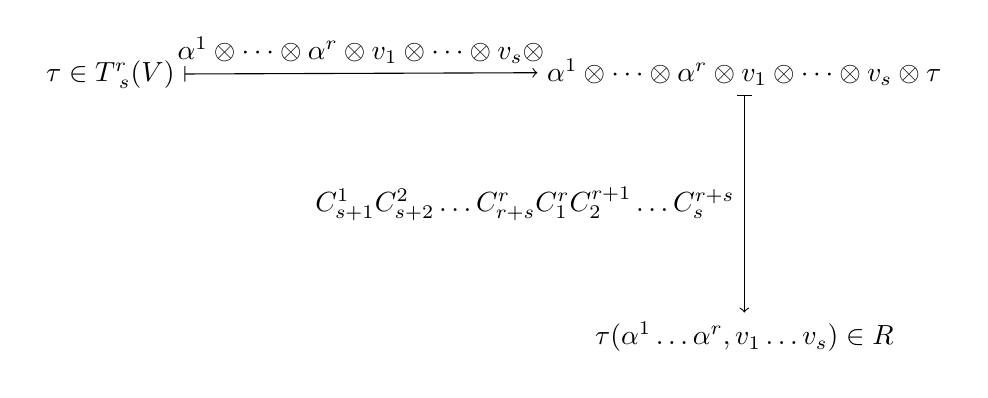
\begin{tikzpicture}
  \matrix (m) [matrix of math nodes, row sep=7.8em, column sep=12.8em, minimum width=5.2em]
  {
  \tau \in T^r_{\,\,s}(V)  &  \alpha^1 \otimes \dots \otimes \alpha^r \otimes v_1\otimes \dots \otimes v_s \otimes \tau  \\ 
& \tau(\alpha^1\dots \alpha^r,v_1\dots v_s)  \in R \\ 
};
  \path[|->]
  (m-1-1) edge node [above] {$ \alpha^1\otimes \dots \otimes \alpha^r \otimes v_1 \otimes \dots \otimes v_s \otimes $} (m-1-2)
  (m-1-2) edge node [left] {$C^1_{ s+1} C^2_{s+2}\dots C^r_{r+s} C^r_1 C_2^{r+1}\dots C_s^{r+s} $} (m-2-2)
  ;
\end{tikzpicture}  
\]
where I've tried to express the right-$R$-module, "right action" on $\alpha^1 \otimes \dots \otimes \alpha^r \otimes v_1\otimes \dots \otimes v_s \in V^*\otimes \dots \otimes V$.  


Conlon (2008) \cite{Conl2008}

\part{Lie Groups, Lie Algebra}

\section{Lie Groups}

\begin{description}
	\item Lie Groups 
	\item Groups
	\item Ring
	\item group algebra
	\item Group Ring
	\item Representation Theory
	\item Modules
	\item $kG$-modules
\end{description}

From Sec. 8.1 ``Noncommutative Rings'' of Rotman (2010) \cite{JRotman2010}:

\begin{definition}
	ring $R$ - additive abelian group equipped with multiplication $\begin{aligned} & \quad \\ 
	& R \times R \to R \\
	& (a,b) \mapsto ab \end{aligned}$ s.t. $\forall \, a ,b \in R$
	
	\begin{enumerate}
		\item[(i)] $a(bc) = (ab)c$ 
		\item[(ii)] $a(b+c) = ab+ ac$, $(b+c)a = ba + ca$ 
		\item[(iii)] $\exists \, 1 \in R$ s.t. $\forall \, a \in R$, $1a = a = a1$
	\end{enumerate}
\end{definition}

Example 8.1\cite{JRotman2010}
\begin{enumerate}
	\item[(ii)] group algebra $kG$, $k$ commutative ring, $G$ group, ``its additive abelian group is free $k$-module having basis labeled by elements of $G$, \\
	i.e. $\forall \, a \in kG$, $a = \sum_{g\in G} a_g g$, $a_g \in k$, \, $\forall \, g \in G$, $a_g \neq 0$ for only finitely many $g\in G$.  
	
	define (ring) multiplication $\begin{aligned} & \quad \\ 
	& kG \times kG \to kG \\
	& ab = ab \end{aligned}$ \, $\forall \, a,b \in kG$, $\begin{aligned} & \quad \\ 
	& a = \sum_{g\in G} a_g g \\
	& b = \sum_{h \in G} b_h g \end{aligned}$ to be 
	\[
	\left( \sum_{g \in G} a_g g \right) \left( \sum_{h \in G} b_h h \right) = \sum_{ z\in G} \left( \sum_{ gh = z} a_g b_h \right)z
	\]
	
\end{enumerate}

\begin{definition}
	Given $R$ ring, left $R$-module is (additive) abelian group $M$ equipped with \\
	scalar multiplication $\begin{aligned} & \quad \\
	& R \times M \to M \\
	& (r,m) \mapsto rm \end{aligned}$ s.t. $\forall \, m , m' \in M$, $\forall \, r, r' , 1 \in R$
	\begin{enumerate}
		\item[(i)] $r (m+m') = rm + rm' $ 
		\item[(ii)] $(r+r')m = rm + r'm $ 
		\item[(iii)] $(rr')m = r(r'm)$
		\item[(iv)] $1m = m$
	\end{enumerate}
\end{definition}

EY : 20150922 Example : for $kG$-module $V^{\sigma}$, for $r \in kG$, so $r= \sum_{g\in G} a_g g$ 
\[
\begin{aligned} & R \times M \to M \\
& (r,m) \mapsto rm \end{aligned} \Longrightarrow \begin{aligned} & kG \times V \to V \\
& (r,v) \mapsto tv \end{aligned}
\]
For some representation $\sigma : G \to GL(V)$, 
\[
rv = \sum_{g \in G} a_g g \cdot v =\sum_{g\in G} a_g \sigma_g(v)
\]
So a $kG$-module needs to be associated with some chosen representation.  

Note for $V$ as an additive abelian group, $\forall \, u,v,w \in V$, 
\[
\begin{aligned}
& v+w = w+v, \, (u+v) + w = u+(v+w) \\ 
& v+0 = v \quad \, \forall \, v \in V \text{ for } 0 \in V \\ 
& v+ (-v) =0 \quad \, \forall \, v \in V
\end{aligned}
\]
So a vector space can be an additive abelian group.  

Note that 
\[
\begin{gathered}
r(v+w) = \left( \sum_{g\in G} a_g g \right)(v+w) = \left( \sum_{g \in G} a_g \sigma_g \right)(v+w) = \sum_{g\in G} a_g \sigma_g(v) + \sum_{g\in G} a_g \sigma_g(w) = rv + rw \\ 
(r+r')v = \left( \sum_{g\in G} a_g g + b_g g \right) v =\sum_{g\in G} (a_g \sigma_g + b_g \sigma_g ) v = \sum_{g \in G}a_g \sigma_g(v) + \sum_{g\in G}b_g \sigma_g(v) = rv + r'v 
\end{gathered}
\]
\[
\begin{gathered}
(rr')v = \left( \sum_{g\in G} a_g g \sum_{h \in G} b_h h \right)v = \left( \sum_{z\in G} \sum_{gh = z} a_g b_h z \right) v = \sum_{z\in G} \sum_{gh \in z} a_g b_h \sigma_z(v) = \sum_{g\in G} \sum_{h \in G} a_g b_h \sigma_g \sigma_h (v)
\end{gathered}
\]
since $\sigma(gh) = \sigma(g) \sigma(h) = \sigma_g \sigma_h = \sigma_{gh}$ ($\sigma$ homomorphism)

$1v = \sigma(1) v = 1v = v$



From Sec. 8.3 ``Semisimple Ring'' of Rotman (2010) \cite{JRotman2010}:

\begin{definition}
	$k$-representation of group $G$ is homomorphism
	\[
	\sigma : G \to GL(V)
	\]
	where $V$ is vector field over field $k$
\end{definition}

\begin{proposition}[8.37 Rotman (2010)\cite{JRotman2010}]\label{Prop:Rotman8.37}
	$\forall \, k$-representation $\sigma : G \to GL(V)$ equips $V$ with structure of left $kG$-module, denote module by $V^{\sigma}$.  \\
	Conversely, $\forall \, $ left $kG$-module $V$ determines $k$-representation $\sigma:G \to GL(V)$
\end{proposition}

\begin{proof}
	Given $\begin{aligned} & \quad \\
	\sigma & :G \to GL(V) \\
	\sigma_g =: \sigma(g) & : V \to V \end{aligned}$, 
	
	define 
	\[
	\begin{aligned}
	kG \times V & \to V \\ 
	\left( \sum_{g\in G} a_g g \right) v & = \sum_{g\in G} a_g \sigma_g(v) 
	\end{aligned}
	\]
	
	Let $\begin{aligned} & \quad \\ 
	& v,w \in V \\
	& r,r',1 \in kG \\
	& r = \sum_{g\in G} a_g g \end{aligned}$
	
	\[
	\begin{gathered}
	r(v+w) = \left( \sum_{g\in G} a_g g \right)(v+w) = \left( \sum_{g \in G} a_g \sigma_g \right)(v+w) = \sum_{g\in G} a_g \sigma_g(v) + \sum_{g\in G} a_g \sigma_g(w) = rv + rw \\ 
	(r+r')v = \left( \sum_{g\in G} a_g g + b_g g \right) v =\sum_{g\in G} (a_g \sigma_g + b_g \sigma_g ) v = \sum_{g \in G}a_g \sigma_g(v) + \sum_{g\in G}b_g \sigma_g(v) = rv + r'v 
	\end{gathered}
	\]
	\[
	\begin{gathered}
	(rr')v = \left( \sum_{g\in G} a_g g \sum_{h \in G} b_h h \right)v = \left( \sum_{z\in G} \sum_{gh = z} a_g b_h z \right) v = \sum_{z\in G} \sum_{gh \in z} a_g b_h \sigma_z(v) = \sum_{g\in G} \sum_{h \in G} a_g b_h \sigma_g \sigma_h (v)
	\end{gathered}
	\]
	since $\sigma(gh) = \sigma(g) \sigma(h) = \sigma_g \sigma_h = \sigma_{gh}$ ($\sigma$ homomorphism)
	
	$1v = \sigma(1) v = 1v = v$
	
	Conversely, assume $V$ left $kG$-module.
	
	If $g \in G$, then $v\mapsto gv$ defines $T_g:V \to V$.  $T_g$ nonsingular since $\exists \, T_g^{-1} = T_{g^{-1}}$
	
	Define $\begin{aligned} & \quad \\
	& \sigma : G \to GL(V) \\
	& \sigma: g \mapsto T_g \end{aligned}$ \quad \\
	
	$\sigma$ $k$-representation
	\[
	\begin{aligned}
	& \sigma(gh) = T_{gh} = T_g T_h = \sigma(g)\sigma(h) \\
	& \sigma(gh)(v) = T_{gh}v = ghv = T_gT_h v = \sigma(g)\sigma(h)v \quad \, \forall \, v \in V
	\end{aligned}
	\]
	
\end{proof}

\begin{proposition}
	Let group $G$, let $\sigma, \tau: G \to GL(V)$ be $k$-representations, field $k$.  \\
	If $V^{\sigma}, V^{\tau}$ corresponding $kG$-modules in Prop. \ref{Prop:Rotman8.37} (Prop. 8.37 in Rotman (2010) \cite{JRotman2010}), then \\
	$V^{\sigma} \simeq V^{\tau}$ as $kG$-modules iff $\exists \, $ nonsingular $\varphi :V \to V$ s.t. 
	\[
	\varphi \tau(g) = \sigma(g) \varphi \quad \, \forall \, g \in G
	\]
	
\end{proposition}

\begin{proof}
	If $\varphi : V^{\tau} \to V^{\sigma}$ $kG$-isomorphism, then $\varphi : V \to V$ isomorphism s.t.
	\[
	\varphi( \sum a_g g v ) = (\sum a_g g)\varphi(v) \quad \, \forall \, v \in V, \, \forall \, g \in G
	\]
	in $V^{\tau}$, $\begin{aligned} & \quad \\
	& kG \times V \to V \\
	& gv = \tau(g)(v) \end{aligned}$ \quad \quad \, in $V^{\sigma}$, $\begin{aligned} & \quad \\
	& kG \times V \to V \\
	& gv = \sigma(g)(v) \end{aligned}$ scalar multiplication
	
	\[
	\begin{gathered}
	\Longrightarrow \forall \, g \in G, v\in V, \quad \, \varphi(\tau(g)(v)) = \sigma(g)(\varphi(v))
	\end{gathered}
	\]
	I think 
	\[
	\varphi(gv) = \varphi(\tau(g)(v)) = g\varphi(v) = \sigma(g)\varphi(v)
	\]
	\[
	\Longrightarrow \varphi \tau(g) = \sigma(g) \varphi \quad \, \forall \, g \in G
	\]
	Conversely, if $\exists \, $ nonsingular $\varphi : V \to V$ s.t. $\begin{aligned} & \quad \\ 
	& \varphi \tau (g) = \sigma(g) \varphi \quad \, \forall \, g \in G \\
	& \varphi \tau(g) v = \varphi(\tau(g)v) = \sigma(g)\varphi(v) \quad \, \forall \, g \in G, \, \forall \, v \in V \end{aligned}$
	
	Consider scalar multiplication
	\[
	\begin{gathered}
	kG \times V \to V \\ 
	\sum_{g\in G} a_g g(v) = \sum_{g\in G} a_g \tau_g(v)
	\end{gathered}
	\]
	\[
	\varphi \left( \sum_{g\in G} a_g \tau_g(v) \right) = \varphi \left( \sum_{g\in G} a_g \tau(g) v\right) = \sum_{g\in G} a_g \sigma(g) \sigma(g)\varphi(v) = \left( \sum_{g\in G} a_g g \right) \varphi(v)
	\]
	
\end{proof}

Admittedly, after this exposition from Rotman (2010) \cite{JRotman2010}, I still didn't understand how $kG$-modules relate to representation theory and group rings.  I turned to Baker (2011) \cite{ABaker2011}, which we'll do right now.  Note that I found a lot of links to online resources on representation theory from Khovanov's webpage \url{http://www.math.columbia.edu/~khovanov/resource/}.  

Note, 
\begin{definition}
	vector subspace $W \subseteq V$ is called a \\
	$G$-submodule, $G$-subspace, EY : 20150922 ``invariant'' subspace? \\
	if $\forall \, g \in G$, for representation $\rho : G \to GL_k(V)$, $\rho_g(w) \in W$, \, $\forall \, w \in W$, $\forall \, g \in G$ i.e. closed under ``action of elements of $G$'' with \\
	$\rho_g =: \rho (g): V \to V$
\end{definition}

Given basis $\mathbf{v} = \lbrace v_1 \dots v_n \rbrace$ for $V$, $\text{dim}_kV = n$, $\forall \, g \in G$, 
\[
\rho_g v_j = \rho(g) v_j = r_{kj}(g) v_k
\]
for, indeed, 
\[
\rho_g x^j v_j = \rho(g) x^j v_j = x^j\rho(g) v_j = x^j r_{kj}(g) v_k = r_{kj} x^j v_k
\]
so that 
\[
\begin{aligned}
& \rho : G \to GL_k(V) \\ 
& \rho(g) = [r_{ij}(g)]
\end{aligned}
\]

Example 2.1 (Baker (2011) \cite{ABaker2011}): Let $\rho :G \to GL_k(V)$ where $\text{dim}_kV=1$
\[
\begin{gathered}
\forall \, v \in V, \, v\neq 0 , \forall \, g \in G, \, \lambda_g \in k \text{ s.t. } g \cdot v = \rho_g(v) = \lambda_g v \\ 
\rho(hg) v = \rho_h \rho_g v = \lambda_{hg} v = \lambda_h \lambda_g v \Longrightarrow \lambda_{hg} = \lambda_h \lambda_g
\end{gathered}
\]
$\Longrightarrow \exists \, $ homomorphism $\begin{aligned} & \quad \\
& \Lambda : G \to k^{\times } \\
& \Lambda(g) = \lambda_g \end{aligned}$


From Sec. 2.2 ``$G$-homomorphisms and irreducible representations'' of Baker (2011) \cite{ABaker2011}, suppose $\begin{aligned} & \rho : G \to GL_k(V) \\
& \sigma : G \to GL_k(W) \end{aligned}$ are 2 representations

Many names for the same thing: $G$-equivalent, $G$-linear, $G$-homomorphism, EY : 20150922 $kG$-isomorphic?

If $\forall \, g \in G$, 

\begin{tikzpicture}
\matrix (m) [matrix of math nodes, row sep=3.8em, column sep=4.8em, minimum width=2.2em]
{
	V & V \\
	V & V \\
};
\path[->]
(m-1-1) edge node [above] {$\varphi$} (m-1-2)
edge node [left] {$\tau_g$} (m-2-1)
(m-1-2) edge node [auto]  {$\sigma_g$} (m-2-2)
(m-2-1) edge node [auto]  {$\varphi$} (m-2-2)
;
\end{tikzpicture}  $\Longleftrightarrow  V^{\tau} \overset{\varphi}{\simeq} V^{\sigma}$

Indeed, define 
\[
\begin{aligned}
& \varphi: V^{\tau} \to V^{\sigma} \\ 
& \varphi(v+w) = \varphi(v) + \varphi(w) \\ 
& \varphi(rv) = \varphi( \sum_{g\in G} a_g g \cdot v) = \varphi( \sum_{g \in G} a_g \tau_g(v) ) = \sum_{ g\in G} a_g \varphi(\tau_g(v)) = \sum_{g\in G} a_g \sigma_g \cdot \varphi(v) = r\varphi(v)
\end{aligned}
\]
EY : 20150922 So $\varphi$ is a $kG$-isomorphism between left $kG$ modules $V^{\tau}$ and $V^{\sigma}$ if it's bijective and is ``linear'' in ``scalars'' $r\in kG$, i.e. $\varphi(rv) = r\varphi(v)$.  

Define action of $G$ on $\text{Hom}_k(V,W)$ ($\text{Hom}_k(V,W)$ is the vector space of $k$-linear transformations $V\to W$) \\
$\forall \, f \in \text{Hom}_k(V,W)$, $\begin{aligned} & \quad \\
& f : V \to W \\
& f(v) \in W \end{aligned}$ \quad \, 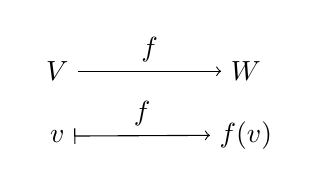
\begin{tikzpicture}
\matrix (m) [matrix of math nodes, row sep=0.8em, column sep=4.8em, minimum width=0.2em]
{
	V & W \\
	v & f(v) \\
};
\path[->]
(m-1-1) edge node [above] {$f$} (m-1-2)
;
\path[|->]
(m-2-1) edge node [auto] {$f$} (m-2-2)
;
\end{tikzpicture}

Consider

\[
\begin{aligned}
& G \times \text{Hom}_k(V,W) \to \text{Hom}_k(V,W) \\ 
& (g\cdot f) \mapsto (\sigma_g f) \circ \rho_{g^{-1}} \text{ i.e. } (g\cdot f)(v) = \sigma_gf(\rho_{g^{-1}}v) \quad \, (f\in \text{Hom}_k(V,W))
\end{aligned}
\]
Let $g,h \in G$, 
\[
(gh \cdot f)(v) = g\cdot \sigma_h f(\rho_{h^{-1}}v) = \sigma_g\sigma_h f\rho_{h^{-1}} \rho_{g^{-1}}(v) = (\sigma_{gh} f \rho_{(gh)^{-1}} )(v)
\]

Thus,  $\begin{aligned} & \quad \\
& G \times \text{Hom}_k(V,W) \to \text{Hom}_k(V,W) \\ 
& (g\cdot f) \mapsto (\sigma_g f)\circ \rho_{g^{-1}} \end{aligned}$ is thus another $G$-representation of $G$.  

For $k$-representation $\rho$, if the only $G$-subspaces of $V$ are $\lbrace 0 \rbrace$, $V$, $\rho$ \textbf{irreducible} or \textbf{simple}.  
\[
\begin{aligned}
& \rho_g(\lbrace 0 \rbrace) = \lbrace 0 \rbrace \\ 
&  \rho_g(V) = V
\end{aligned}
\]


given subrepresentation $W \subseteq V$, $V/W$ admits linear action of $G$, $\overline{\rho}_W : G \to GL_k(V/W)$ quotient representation 
\[
\overline{\rho}_W(g)(v+W) = \rho(g)(v) + W
\]
if $v'-v \in W$
\[
\rho(g)(v') + W = \rho(g)(v+(v'-v))+W = (\rho(g)(v) + \rho(g)(v'-v) ) + W = \rho(g)(v) + W
\]
\begin{proposition}[2.7 Baker (2011)\cite{ABaker2011}] \label{Prop:Baker2.7}
	if $f:V \to W$ $G$-homomorphism, then
	\begin{enumerate}
		\item[(a)] $\text{ker}{f}$ is $G$-subspace of $V$ 
		\item[(b)] $\text{im}{f}$ is $G$-subspace of $W$
	\end{enumerate}
\end{proposition}

\begin{proof}
	Recall 
	\begin{tikzpicture}
	\matrix (m) [matrix of math nodes, row sep=3.8em, column sep=4.8em, minimum width=2.2em]
	{
		V & W \\
		V & W \\
	};
	\path[->]
	(m-1-1) edge node [above] {$f$} (m-1-2)
	edge node [left] {$\rho_g$} (m-2-1)
	(m-1-2) edge node [auto]  {$\sigma_g$} (m-2-2)
	(m-2-1) edge node [auto]  {$f$} (m-2-2)
	;
	\end{tikzpicture}
	
	\begin{enumerate}
		\item[(a)] Let $v\in \text{ker}{f}$.  Then $\forall \, g \in G$, 
		\[
		f(\rho_g v) = \sigma_g f(v) = 0 
		\]
		so $\rho_g v \in \text{ker}{f}$, $\forall \, g \in G$.  So $\text{ker}{f}$ is $G$-subspace of $V$
		\item[(b)] Let $w\in \text{im}{f}$.  So $w = f(u)$ for some $u \in V$ 
		\[
		\sigma_g w = \sigma_g f(u) = f(\rho_gu) \in \text{im}f
		\]
		So $\text{im}{f}$ is $G$-subspace of $W$
	\end{enumerate}
\end{proof}

\begin{theorem}[Schur's Lemma]
	Let $\begin{aligned} & \quad \\
	& \rho : G \to GL_{\mathbb{C}}(V) \\
	& \sigma : G \to GL_{\mathbb{C}}(W) \end{aligned}$ be irreducible representations of $G$ over field $k= \mathbb{C}$; let $f:V \to W$ be $G$-linear map.  
	
	\begin{enumerate}
		\item[(a)] if $f\neq 0$, $f$ isomorphism.  True $\forall \, k$ field, not just $\mathbb{C}$
		\item[(b)] if $V=W$, $\rho = \sigma$, then for some $\lambda \in \mathbb{C}$, $f$ given by $f(v) = \lambda v$ ($v\in V$) (true for algebraically closed fields)
	\end{enumerate}
\end{theorem}

\begin{proof}
	\begin{enumerate}
		\item[(a)] By Prop. \ref{Prop:Baker2.7}, $\text{ker}f \subseteq V$, $\text{im}f \subseteq W$ are $G$-subspaces.  \\
		For $\rho$, only $G$-subspaces are $0$ or $V$, so if $\text{ker}f = V$, $f=0$.  If $\text{ker}f = 0$, $f$ injective.  \\
		For $\sigma$, only $G$-subspaces are $0$ or $V$, so $\text{im}f =0 $, $f=0$.  If $\text{im}f =V$, $f$ surjective.  
		
		$\Longrightarrow f$ isomorphism.  
		\item[(b)] Let $\lambda \in \mathbb{C}$ be an eigenvalue of $f$, $f(v_0) = \lambda v_0$ eigenvector, $v_0 \neq 0$.  
		
		Let linear $f_{\lambda} : V \to V$ s.t. 
		\[
		f_{\lambda}(v) = f(v) - \lambda v \quad \, (v\in V)
		\]
		$\forall \, g \in G$
		\[
		\rho_g f_{\lambda}(v) = \rho_gf(v) - \rho_g \lambda v = f(\rho_g v) - \lambda \rho_g v= f_{\lambda}(\rho_g v)
		\]
		So $f_{\lambda}$ is $G$-linear, for 
		
		\begin{tikzpicture}
		\matrix (m) [matrix of math nodes, row sep=3.8em, column sep=4.8em, minimum width=2.2em]
		{
			V & V \\
			V & V \\
		};
		\path[->]
		(m-1-1) edge node [above] {$f$} (m-1-2)
		edge node [left] {$\rho_g$} (m-2-1)
		(m-1-2) edge node [auto]  {$\rho_g$} (m-2-2)
		(m-2-1) edge node [auto]  {$f$} (m-2-2)
		;
		\end{tikzpicture}
		
		Since $f_{\lambda}(v_0) =0$, by Prop. \ref{Prop:Baker2.7}, $\text{ker}f_{\lambda} = V$, (for $\text{ker}f_{\lambda}\neq 0$ and so $\text{ker}f_{\lambda}=V$)
		
		By rank-nullity theorem, $\text{dim}V = \text{dim}\text{ker}f_{\lambda} + \text{dim}\text{im}f_{\lambda}$.  
		
		So $\text{im}f_{\lambda}=0$, and so $f_{\lambda}(v)=0$ ($\forall \, v \in V$) $\Longrightarrow f(v) = \lambda v$
	\end{enumerate}
\end{proof}

Schur's lemma, at least the first part, implies that the left $kG$-modules associated with representations $\rho, \sigma$ are $kG$-isomorphic, i.e.

\[
\begin{gathered}
\begin{tikzpicture}
\matrix (m) [matrix of math nodes, row sep=3.8em, column sep=4.8em, minimum width=2.2em]
{
	V & W \\
	V & W \\
};
\path[->]
(m-1-1) edge node [above] {$f$} (m-1-2)
edge node [left] {$\rho_g$} (m-2-1)
(m-1-2) edge node [auto]  {$\sigma_g$} (m-2-2)
(m-2-1) edge node [auto]  {$f$} (m-2-2)
;
\end{tikzpicture}  \Longleftrightarrow  V^{\rho} \overset{f}{\simeq} V^{\sigma}
\end{gathered}
\]

with $f$ being an isomorphism between $V^{\rho}$ and $V^{\sigma}$ s.t. 
\[
\begin{gathered}
f(v+w) = f(v) + f(w) \quad \, \forall \, v,w \in (V^{\sigma},+) \\ 
f(rv) = rf(v) \quad \, \forall \, r  = \sum_{g \in G} a_g g \in kG
\end{gathered}
\]

Kosmann-Schwarzbach's \textbf{Groups and Symmetries}\cite{YKosmann-Schwarzbach2010} is a very lucid text that's mathematically rigorous enough and practical for physicists.  It's really good and very clear.  Let's follow its development for $SU(2), SO(3), SL(2,\mathbb{C})$ and corresponding Lie algebras $\mathfrak{su}(2)$, $\mathfrak{so}(3)$, $\mathfrak{sl}(2,\mathbb{C})$.  

From Chapter 2 ``Representations of Finite Groups'' of Kosmann-Schwarzbach (2010) \cite{YKosmann-Schwarzbach2010}

\begin{definition}[2.1 Kosmann-Schwarzbach (2010)\cite{YKosmann-Schwarzbach2010}] \label{Def:2.1scalarproductG}
	On $L^2(G)$, scalar product defined by 
	\[
	\langle f_1 | f_2 \rangle = \frac{1}{|G|} \sum_{g\in G} \overline{f_1(g)} f_2(g)
	\]
	$f_1,f_2 \in \mathcal{F}(G) \equiv \mathbb{C}[G]$ vector space of functions on $G$ taking values on $\mathbb{C}$
\end{definition}

\begin{definition}[2.3 Kosmann-Schwarzbach (2010)\cite{YKosmann-Schwarzbach2010}]
	Let $(E,\rho)$ be representation of $G$ \\
	character of $\begin{aligned} & \quad \\ 
	\rho \equiv \chi_{\rho} & : G \to \mathbb{C} \\
	\chi_{\rho}(g) & = \text{tr}( \rho(g)) = \sum_{i=1}^n (\rho(g))_{ii} \end{aligned}$ 
	
	Note: equivalent representations have same character \\
	each conjugacy class of $G$, function $\chi_p$ is constant
\end{definition}

Looking at Def. \ref{Def:2.1scalarproductG}
\[
\langle \chi_{\rho_1} | \chi_{\rho_2} \rangle = \frac{1}{|G| } \sum_{g\in G} \chi_{\rho_1}(g^{-1}) \chi_{\rho_2(g)}
\]
since $\overline{\chi_{\rho_1(g)}} = \chi_{\rho_1}(g^{-1})$ by unitarity of representation with respect to scalar product $\langle \, , \, \rangle$

\begin{proposition}[2.7 Kosmann-Schwarzbach (2010)\cite{YKosmann-Schwarzbach2010}]
	Let $\begin{aligned} & \quad \\ 
	& (E_1, \rho_1) \\
	& (E_2, \rho_2) \end{aligned}$ be representations of $G$, let linear $u: E_1 \to E_2$.  
	
	Then $\exists \, $ linear $T_u$ s.t. 
	
	\begin{equation}\label{Eq:T_ucharacters}
	\begin{aligned} & \quad \\
	& T_u : E_1 \to E_2 \\
	& T_u = \frac{1}{|G|} \sum_{g\in G} \rho_2(g)u\rho_1(g)^{-1} \end{aligned}
	\end{equation}
	
	so that $\rho_2(g) T_u = T_u\rho_1(g) \quad \, \forall \, g \in G$
\end{proposition}

\begin{proof}
	\[
	\rho_2(g) T_u = \frac{1}{|G|} \sum_{ h \in G } \rho_2(gh) u \rho_1(h^{-1}) = \frac{1}{|G|} \sum_{ k \in G} \rho_2(k) u \rho_1(k^{-1}g) = T_u \rho_1(g)
	\]
\end{proof}

Thus, diagrammatically, we have that 
\[
\begin{tikzpicture}
\matrix (m) [matrix of math nodes, row sep=3.8em, column sep=4.8em, minimum width=2.2em]
{
	E_1 & E_2 \\
};
\path[->]
(m-1-1) edge node [above] {$u$} (m-1-2)
;
\end{tikzpicture} \Longrightarrow  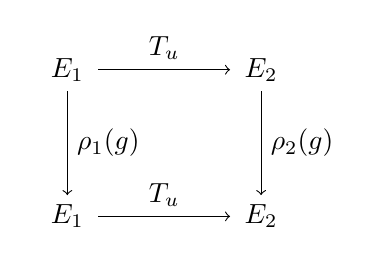
\begin{tikzpicture}
\matrix (m) [matrix of math nodes, row sep=3.8em, column sep=4.8em, minimum width=2.2em]
{
	E_1 & E_2 \\
	E_1 & E_2 \\
};
\path[->]
(m-1-1) edge node [above] {$T_u$} (m-1-2)
edge node [auto] {$\rho_1(g)$} (m-2-1)
(m-1-2) edge node [auto]  {$\rho_2(g)$} (m-2-2)
(m-2-1) edge node [auto]  {$T_u$} (m-2-2)        
;
\end{tikzpicture}
\]

From Definition	1.12 of	Kosmann-Schwarzbach \cite{YKosmann-Schwarzbach2010}, ``representations $\rho_1$ and $\rho_2$ are called \textbf{equivalent} if there is a bijective intertwining operator for $\rho_1$ and $\rho_2$.''  So I will interpret this as if an intertwining operator is not bijective, then the representations $\rho_1$, $\rho_2$ are not equivalent.  

\begin{proposition}[2.8 Kosmann-Schwarzbach (2010)\cite{YKosmann-Schwarzbach2010}]
	Let $\begin{aligned}
	& \quad \\
	& (E_1,\rho_1) \\
	& (E_2,\rho_2) \end{aligned}$ be irreducible representations of $G$, let linear $u:E_1 \to E_2$, define $T_u$ by $T_u = \frac{1}{ |G|} \sum_{g\in G} \rho_2(g) u \rho_1(g)^{-1}$ by Eq. \ref{Eq:T_ucharacters}.  
	
	\begin{enumerate}
		\item[(i)] If $\rho_1$, $\rho_2$ inequivalent, then $T_u=0$
		\item[(ii)] If $E_1=E_2= E$ and $\rho_1 = \rho_2 = \rho$, then
		\[
		T_u = \frac{\text{tr}{(u)}}{ \text{dim}E} 1_E
		\]
	\end{enumerate}
\end{proposition}

\begin{proof}
	\begin{enumerate}
		\item[(i)] if $\rho_1,\rho_2$ are inequivalent, by definition, $T_u$ is not isomorphic.  Then by Schur's lemma (first part), $T_u=0$
		\item[(ii)] By Schur's lemma, $T_u(v) = \lambda v$ \, $\forall \, v \in E = E_1 = E_2$.  So $T_u = \lambda 1_E$.  $\text{tr}T_u = \lambda \text{dim}E$ or $\lambda = \frac{ \text{tr}T_u}{ \text{dim}E}$.  Thus, $T_u = \frac{\text{tr}{T_u}}{ \text{dim}E}1_E$
	\end{enumerate}
\end{proof}

Let $\begin{aligned} & \quad \\
& (e_1 \dots e_n) \text{ basis of $E$ } \\
& (f_1 \dots f_p) \text{ basis of $F$ } \end{aligned}$ 

$\forall \, u \in \mathcal{L}(E,F)$, $\begin{aligned} & \quad \\
& u : E \to F \\
& u(x) = u(x^j e_j) = x^ju(e_j) = x^ju^i_{ \,\, j}f_i \\
& u = u^i_{ \,\, j} e^j \otimes f_i \end{aligned}$ for $\begin{aligned} & \quad \\ 
& x = x^j e_j \in E \\
& y = y^i f_i \in F \end{aligned}$

For 
\[
\begin{aligned}
& T : E^* \otimes F \to \mathcal{L}(E,F) \\
& T(\xi \otimes y) = u^i_{ \,\,j}e^j \otimes f_i \text{ i.e. set $T(\xi \otimes y)$ to this $u$} \\
& T(\xi \otimes y) = T(\xi_l e^l \otimes y^k f_k) = \xi_l y^k T(e^l \otimes f_k) = (\xi_l y^k T^{li}_{ \,\, kj} ) e^j \otimes f_i \Longrightarrow \xi_l y^k T^{li}_{ \,\, kj} = u^i_{ \,\, j}
\end{aligned}
\]

\subsubsection*{Exercises}

Exercises of Ch. 2 Representations of Finite Groups \cite{YKosmann-Schwarzbach2010}

\exercisehead{2.6}\cite{YKosmann-Schwarzbach2010} \emph{The dual representation}.  

Let $(E,\pi)$ representation of group $G$.  \\
$\forall \, g \in G$, $\xi \in E^*$, $x\in E$, set $\langle \pi^*(g)(\xi), x \rangle = \langle \xi, \pi(g^{-1})(x) \rangle$
\begin{enumerate}
	\item[(a)] \emph{dual} (or \emph{contragredient}) of $\pi$, $\pi^*:G \to \text{End}(E^*)$, $\pi^*$ is a representation, since
	\[
	\begin{gathered}
	\langle \pi^*(gh)(\xi),x\rangle = \langle \xi, \pi((gh)^{-1})(x) \rangle = \langle \xi, \pi(h^{-1}g^{-1})(x) \rangle = \langle \xi, \pi(h^{-1}) \pi(g^{-1})(x) \rangle = \langle \xi, \pi(h^{-1}) (\pi(g^{-1})(x)) \rangle =  \\
	= \langle \pi^*(h)(\xi), \pi(g^{-1})(x) \rangle = \langle \pi^*(g)\pi^*(h)(\xi), x \rangle
	\end{gathered}
	\]
	since this is true, $\forall \, x \in E$, $\forall \, \xi \in E^*$, $\pi^*(gh) = \pi^*(g)\pi^*(h)$.  
	
	dual $\pi^*$ of $\pi$ is a representation.  
	
	\item[(b)]
	
	Consider $\begin{aligned} & \quad \\
	& G \times \mathcal{L}(E,F) \to \mathcal{L}(E,F) \\
	& g\cdot u = \rho(g) \circ u \circ \pi(g^{-1}) \end{aligned}$.  
	
	Define 
	\[
	\begin{aligned}
	& \sigma : G \to \text{End}(\mathcal{L}(E,F)) \\ 
	& \sigma(g):\mathcal{L}(E,F) \to \mathcal{L}(E,F) \\  
	& \sigma(g)(u) = \rho(g)\circ u \circ \pi(g^{-1})
	\end{aligned}
	\]
	
	Let $(e_1 \dots e_n)$ be a basis of $E$.  Let $\xi = \xi_i e^i \in E^*$, $x = x^j e_j \in E$.  
	
	Consider the isomorphism $T: E^*\otimes F \to \mathcal{L}(E,F)$ defined as\footnote{\emph{Mathematics stackexchage} \href{http://math.stackexchange.com/questions/428185/isomorphism-between-hom-and-tensor-product}{Isomorphism between Hom and tensor product [duplicate]} \url{http://math.stackexchange.com/questions/428185/isomorphism-between-hom-and-tensor-product} \\ \url{http://math.stackexchange.com/questions/57189/understanding-isomorphic-equivalences-of-tensor-product}}
	
	\[
	\begin{aligned}
	& T: E^*\otimes F \to \mathcal{L}(E,F) = \text{Hom}(E,F) \\
	& \xi \otimes y  \mapsto (x \mapsto \xi(x)y)
	\end{aligned}
	\]
	
	Choose bases $\begin{aligned} & \quad \\
	& (e_1 \dots e_n) \text{ of } E \\
	& (e^1 \dots e^n) \text{ of } E^* \\  
	& (f_1 \dots f_p) \text{ of } F 
	\end{aligned}$.  Then
	\[
	\begin{aligned}
	& T(e^j\otimes f_i)(x) = T(e^j\otimes f_i)(x^ke_k) = \delta^j_{\,\,k} x^k f_i = x^j f_i \\
	& T(e^j\otimes f_i)(e_k) = \delta^j_{\,\,k}f_i
	\end{aligned}
	\]
	
	Consider 
	\[
	\begin{aligned} & \quad \\
	& u \in \mathcal{L}(E,F) \\
	& u: E \to F \\
	& u(x) = u(x^je_j) = x^ju(e_j) = x^j u^i_{\,\,j} f_i \\
	& u(e_j) = u^i_{\,\,j}f_i \text{ i.e. } u: e_j \to u^i_{\,\,j}f_i \end{aligned}
	\]
	
	Then $\forall u \in \mathcal{L}(E,F)$,
	\[
	\begin{gathered}
	T(u^i_{\,\, j} e^j \otimes f_i)(e_k) = u^i_{\,\,j}\delta^j_{\,\,k}f_i = u^i_{\,\,k}f_i = u(e_k) \Longrightarrow u = T(u^i_{\,\,j}e^j\otimes f_i)
	\end{gathered}
	\]
	so $T$ is surjective.  
	
	With $T(\xi\otimes y) = T(\xi'\otimes y')$, 
	\[
	\begin{gathered}
	T(\xi\otimes y)(x) = T(\xi' \otimes y')(x) \\
	\xi(x)y = \xi'(x)y' \Longrightarrow \xi(x)y - \xi'(x)y' = 0 
	\end{gathered}
	\]
	which implies that $\xi\otimes y = \xi'\otimes y'$.  So $T$ is injective.  Or, one could consider that $T^{-1} : \mathcal{L}(E,F) \to E^*\otimes F$, $T^{-1} : u \mapsto u^i_{\,\,j}e^j\otimes f_i$, which is the inverse of $T$.  
	
	\begin{remark}
		\[
		\begin{aligned}
		& E^* \otimes F \overset{T}{\simeq} \mathcal{L}(E,F) = \text{Hom}(E,F) \\ 
		& (\xi, y) \mapsto (x \mapsto \xi(x)y) 
		\end{aligned}
		\]
		and so $(e^j \otimes f_i) \mapsto (x\mapsto e^j(x)f_i = x^jf_i)$
		
		So $E^*\otimes F$ is isomorphic to $\mathcal{L}(E,F) = \text{Hom}(E,F)$
	\end{remark}
	
	For representation $\pi$, 
	\[
	\begin{aligned}
	& \pi:G \to \text{End}(E) \\ 
	& \pi(g):E \to E \\ 
	&  \pi(g)(x) = \pi(g)(x^j e_j) = x^j \pi(g)(e_j) = x^j \pi(g)^i_{ \,\, j} e_i = (\pi(g)^i_{\,\,j} x^j e_i
	\end{aligned}
	\]
	
	Consider this matrix formulation:
	\[
	\begin{gathered}
	\pi^*(g)(\xi) = \pi^*(g)(\xi_i e^i) = \xi_i \pi^*(g)(e^i) = \xi_i (\pi^*(g))^i_{\,\,j}e^j \\
	\Longrightarrow \langle \pi^*(g)(\xi), x \rangle = \xi_i (\pi^*(g))^i_{ \,\, j}x^j
	\end{gathered}
	\]
	and 
	\[
	\langle \xi, \pi(g^{-1})(x) \rangle = \xi_i \pi(g^{-1})^i_{ \,\, j}x^j 
	\]
	so that 
	\[
	\langle \pi^*(g)(\xi),x \rangle = \langle \xi, \pi(g^{-1})(x) \rangle \Longrightarrow \pi(g^{-1})^i_{\,\, j} = (\pi^*(g))^i_{ \,\, j}
	\]
	Thus, given a choice of basis for $E$, the \emph{dual} of $\pi$, $\pi^*(g)^i_{\,\,j}$, and $\pi(g^{-1})^i_{\,\,j}$ are formally equal.  
	
	So for a choice of basis of $E$ and of $F$, 
	\[
	\begin{gathered}
	(\pi^*\otimes \rho)(g)(\xi,y) = (\pi^*(g)\otimes \rho(g))(\xi,y) = \pi^*(g)\xi \otimes \rho(g)y = \xi_l \pi(g^{-1})^l_{\,\,j} e^j \otimes \rho(g)^i_{\,\,k}y^k f_i = \rho(g)^i_{\,\,k}y^k \xi_l \pi(g^{-1})^l_{\,\,j} e^j \otimes f_i
	\end{gathered}
	\]
	Applying $T$,
	\[
	T(\pi^*\otimes \rho)(g)(\xi,\rho) = \rho(g)^i_{\,\,k} y^k \xi_l \pi(g^{-1})^l_{\,\,j} = \rho(g)T(\xi,y) \pi(g^{-1})
	\]
	
	Thus 
	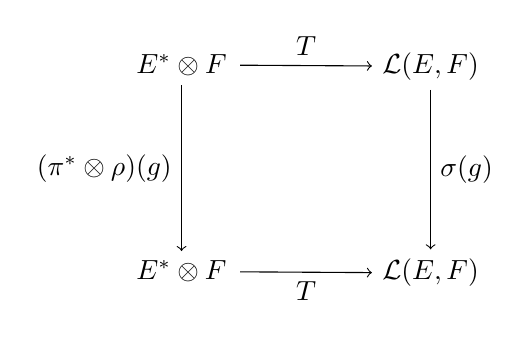
\begin{tikzpicture}
	\matrix (m) [matrix of math nodes, row sep=5.8em, column sep=4.8em, minimum width=4.2em]
	{
		E^*\otimes F & \mathcal{L}(E,F) \\ 
		E^*\otimes F & \mathcal{L}(E,F) \\ 
	};
	\path[->]
	(m-1-1) edge node [above] {$T$} (m-1-2)
	edge node [left] {$(\pi^*\otimes \rho)(g)$} (m-2-1)
	(m-1-2) edge node [auto]  {$\sigma(g)$} (m-2-2)
	(m-2-1) edge node [below] {$T$} (m-2-2)
	;
	\end{tikzpicture} \quad \quad \quad \, 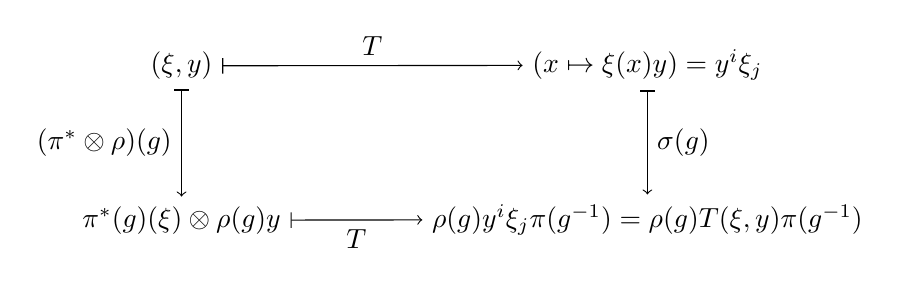
\begin{tikzpicture}
	\matrix (m) [matrix of math nodes, row sep=3.8em, column sep=4.8em, minimum width=2.2em]
	{
		(\xi,y) & (x\mapsto \xi(x) y) = y^i \xi_j \\
		\pi^*(g)(\xi) \otimes \rho(g)y & \rho(g) y^i \xi_j \pi(g^{-1}) = \rho(g) T(\xi,y) \pi(g^{-1}) \\
	};
	\path[|->]
	(m-1-1) edge node [above] {$T$} (m-1-2)
	edge node [left] {$(\pi^*\otimes \rho)(g)$} (m-2-1)
	(m-1-2) edge node [auto]  {$\sigma(g)$} (m-2-2)
	(m-2-1) edge node [below] {$T$} (m-2-2)
	;
	\end{tikzpicture}
	Thus, representation $\sigma(g)$ is equivalent to representation $(\pi^*\otimes \rho)$, a tensor product of representations.  
	
\end{enumerate}

\exercisehead{2.15} \emph{Representation of $GL(2, \mathbb{C})$ on the polynomials of degree 2}

Let group $G$, let representation $\rho$ of $G$ on $V= \mathbb{C}^n$, i.e. $\rho : G \to \text{End}(V)$ \\
Let $P^{(k)}(V)$ vector space of complex polynomials on $V$ that are homogeneous of degree $k$. 

For $f\in P^{(k)}(V)$, the general form is 
\[
f = \sum_{ \substack{ i_1 + i_2 + \dots + i_n = k \\ 0 \leq i_j \leq k } } a_{i_1 i_2 \dots i_d} x_1^{i_1} x_2^{i_2} \dots x_n^{i_n}
\]

Given 
\[
\binom{n+k}{k} = \binom{k-1}{k-1} + \binom{k}{k-1} + \dots + \binom{n+k-1}{k-1} = \sum_{i=0}^n \binom{k-1+i}{k-1}
\]
$\binom{k+n-1}{n-1}$ is number of monomials of degree $k$.  

So $\text{dim}P^{(k)}(V) = \binom{k+n-1}{n-1}$.   This is a very lucid and elementary exposition on the basics of polynomials which I found was useful for the basic facts I forgot\footnote{Polynomials. Math 4800/6080 Project Course \url{http://www.math.utah.edu/~bertram/4800/PolyIntroduction.pdf}}.

So we have the graded algebra
\[
P(V) = \bigoplus_{k=0}^{\infty} P^{(k)}(V)
\]

\[
\begin{aligned}
& \rho^{(k)}: G \to \text{End}(P^{(k)}(V)) \\ 
& \rho^{(k)}(g): P^{(k)}(V) \to P^{(k)}(V) \\ 
& \rho^{(k)}(g)(f) = f\circ \rho(g^{-1})
\end{aligned}
\]
This is a representation of $G$ since 
\begin{enumerate}
	\item[(a)] 
	\[
	\begin{gathered}
	\begin{aligned}
	& \rho^{(k)}(gh)(f) = f\circ \rho((gh)^{-1}) = f\circ \rho(h^{-1}g^{-1}) = f\circ \rho(h^{-1}\rho(g^{-1}) \\ 
	& \rho^{(k)}(g) \rho^{(k)}(h)(f) = \rho^{(k)}(g) (f\circ \rho(h^{-1})) = f\circ \rho(h^{-1})\circ \rho(g^{-1})
	\end{aligned} \Longrightarrow \rho^{(k)}(gh) = \rho^{(k)}(g) \rho^{(k)}(h)
	\end{gathered}
	\]
	
	
	\item[(b)]
	Choose basis $(e_1 \dots e_n)$ of $V$, $x = x^j e_j \in V$, $\rho : G \to \text{End}(V)$, and so $\rho(g)(x) = \rho(g)(x^je_j) = x^j\rho(g)(e_j)= x^j(\rho(g))^i_{ \,\, j} e_i$.  \\
	With $\xi(e_i) = \xi_i \Longrightarrow \langle \xi, \rho(g^{-1})x\rangle = \xi_i x^j (\rho(g^{-1}))^i_{ \,\, j}$
	
	$\forall \, \xi \in V^*$, $\xi = \xi_i e^i$, 
	\[
	\begin{gathered}
	\rho^*(g)(\xi) = \rho^*(g)(\xi_i e^i) = \xi_i \rho^*(g)^i_{\,\,j} e^j \\ 
	\Longrightarrow   \langle \rho^*(g)(\xi), x \rangle = \xi_i x^j (\rho^*(g))^i_{ \,\,j} \Longrightarrow (\rho^*(g))^i_{\,\,j} = (\rho(g^{-1}))^i_{ \,\, j} 
	\end{gathered}
	\]
	
	So $\forall \, f \in P^{(1)}(V)$, $x\in V$, $\rho(g^{-1})x = x^j(\rho(g^{-1}))^i_{\,\,j} e_i$.  So $f\circ \rho(g^{-1})(x) = \sum_{i=1}^n a_i(\rho(g^{-1}))^i_{\,\,j} x^j = \sum_{i=1}^n a_i(\rho^*(g))^i_{\,\,j} x^j$ \\
	$\Longrightarrow \rho^{(1)}(g)(f) = f\circ \rho^*(g)$
	\item[(c)] Suppose $G= GL(2,\mathbb{C})$, $V=\mathbb{C}^2$, $\rho$ fundamental representation $g= \left( \begin{matrix} a & b \\
	c & d \end{matrix} \right)$, $g^{-1} = \frac{1}{\text{det}g} \left( \begin{matrix} d & -b \\
	-c & a \end{matrix} \right)$ for $\text{det}g = ad-bc$.  
	
	Let $k=2$, $\text{dim}P^{(2)}(\mathbb{C}^2) = \binom{2+2-1}{2-1} = \binom{3}{1} = 3$
	
	$\forall \, f \in P^{(2)}(\mathbb{C}^2)$, $f(x,y) = Ax^2 + 2Bxy + Cy^2$ \\
	Let 
	\[
	\begin{gathered}
	P^{(2)}(\mathbb{C}^2) \to \mathbb{C}^3 \\ 
	f(x,y) = Ax^2 + 2Bxy + Cy^2 \mapsto \left( \begin{matrix} A \\ B \\ C \end{matrix} \right) \in \mathbb{C}^3
	\end{gathered}
	\]
	Call this transformation $T$, $T: P^{(2)}(\mathbb{C}^2) \to \mathbb{C}^3$.  
	
	$\forall \, \left( \begin{matrix} A \\ B \\ C \end{matrix} \right) \in \mathbb{C}^3$, $f(x,y) = Ax^2 + 2Bxy + Cy^2$ and $Tf(x,y) = \left( \begin{matrix} A \\ B \\ C \end{matrix} \right)$.  $T$ surjective.  
	
	Suppose $Tf(x,y) = Tf'(x,y)$, 
	\[
	\begin{gathered}
	\Longrightarrow Ax^2 + 2Bxy + Cy^2 = A'x^2 + 2B'xy + C'y^2 \\ 
	\Longrightarrow (A-A')x^2 + 2(B-B')xy + (C-C')y^2 = 0
	\end{gathered}
	\]
	Then since the monomials form a basis, and its basis elements are independent (by definition), then $A=A'$, $B=B'$, $C=C'$.  $T$ injective.  So $T$ is bijective, an isomorphism.  
	
	(This is all in \verb|groups.sage|)
	\begin{lstlisting}
	sage: P2CC.<x,y> = PolynomialRing(CC,2) # this declares a PolynomialRing of field of complex numbers, 
	# of order 2 (i.e. only 2 variables for a polynomial, such as x, y)
	sage: A = var('A')
	sage: assume(A,''complex'')
	sage: B = var('B')
	sage: assume(B,''complex'')
	sage: C = var('C')
	sage: assume(C,''complex'')
	sage: f(x,y) = A*x**2 +2*B*x*y + C*y**2
	
	sage: a = var('a')
	sage: assume(a,''complex'')
	sage: b = var('b')
	sage: assume(b,''complex'')
	sage: c = var('c')
	sage: assume(c,''complex'')
	sage: d = var('d')
	sage: assume(d,''complex'')
	sage: g = Matrix([[a,b],[c,d]] )
	sage: X = Matrix([[x],[y]])
	sage: f( (g.inverse()*X)[0,0], (g.inverse()*X)[1,0] ).expand()
	sage: f( (g.inverse()*X)[0,0], (g.inverse()*X)[1,0] ).expand().coefficient(x^2).full_simplify()
	(C*c^2 - 2*B*c*d + A*d^2)/(b^2*c^2 - 2*a*b*c*d + a^2*d^2)
	sage: f( (g.inverse()*X)[0,0], (g.inverse()*X)[1,0] ).expand().coefficient(x*y).full_simplify()
	-2*(C*a*c + A*b*d - (b*c + a*d)*B)/(b^2*c^2 - 2*a*b*c*d + a^2*d^2)
	sage: f( (g.inverse()*X)[0,0], (g.inverse()*X)[1,0] ).expand().coefficient(y^2).full_simplify()
	(C*a^2 - 2*B*a*b + A*b^2)/(b^2*c^2 - 2*a*b*c*d + a^2*d^2)
	\end{lstlisting}
	
	So 
	\[
	\begin{gathered}
	\rho^{(2)}(g)(f)(x,y) = f\circ \rho(g^{-1})(x,y) = \\
	= \frac{ Cc^2 - 2Bcd + Ad^2}{(ad-bc)^2}x^2 + - 2 \frac{ (Cac + Abd - (bc+ad) B)}{(ad-bc)^2} xy + \frac{ Ca^2 - 2Bab + Ab^2 }{(ad-bc)^2 } y^2
	\end{gathered}
	\]
	
	So define $\widetilde{ \rho}: G \to \text{End}(\mathbb{C}^3)$. $\widetilde{\rho}$ is a representation, for 
	\[
	\begin{gathered}
	\forall v = \left( \begin{matrix} A \\ B \\ C \end{matrix} \right) \in \mathbb{C}^3, \quad \, \widetilde{\rho}(gh)(v) = T \circ f \circ \rho((gh)^{-1}) = T\circ f \circ \rho(h^{-1}g^{-1}) = T\circ f \circ \rho(h^{-1}) \rho(g^{-1}) \\ 
	\text{ Now } \widetilde{\rho}(h)(v) = T\circ f \circ \rho(h^{-1}) \\
	\Longrightarrow \widetilde{\rho}(g) \widetilde{\rho}(h)(v) = T \circ (f\circ \rho(h^{-1}))\circ \rho(g^{-1}) = T\circ f \circ \rho(h^{-1}) \rho(g^{-1}) \text{ and so }\\
	\widetilde{\rho}(gh) = \widetilde{\rho}(g) \widetilde{\rho}(h)
	\end{gathered}
	\]
	
	And so 
	\[
	\widetilde{\rho}^*(g)(v) = Tf\rho(g^{-1})
	\]
	and consider this commutation diagram, that (helped me at least and) clarifies the relationships:
	
	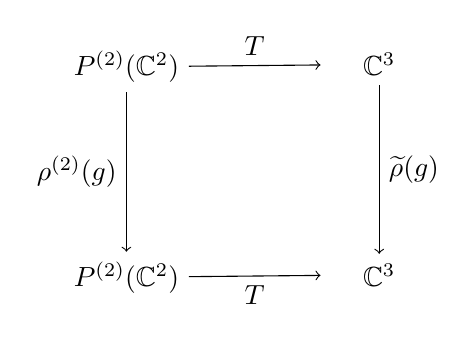
\begin{tikzpicture}
	\matrix (m) [matrix of math nodes, row sep=5.8em, column sep=4.8em, minimum width=4.2em]
	{
		P^{(2)}(\mathbb{C}^2) & \mathbb{C}^3 \\ 
		P^{(2)}(\mathbb{C}^2) & \mathbb{C}^3 \\ 
	};
	\path[->]
	(m-1-1) edge node [above] {$T$} (m-1-2)
	edge node [left] {$\rho^{(2)}(g)$} (m-2-1)
	(m-1-2) edge node [auto]  {$\widetilde{\rho}(g)$} (m-2-2)
	(m-2-1) edge node [below] {$T$} (m-2-2)
	;
	\end{tikzpicture} \quad \quad \quad \, 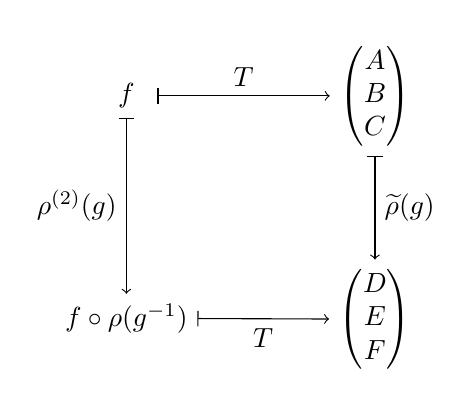
\begin{tikzpicture}
	\matrix (m) [matrix of math nodes, row sep=3.8em, column sep=4.8em, minimum width=2.2em]
	{
		f & \left( \begin{matrix} A \\ B \\ C \end{matrix} \right) \\ 
		f\circ \rho(g^{-1}) & \left( \begin{matrix} D \\ E \\ F \end{matrix} \right) \\ 
	};
	\path[|->]
	(m-1-1) edge node [above] {$T$} (m-1-2)
	edge node [left] {$\rho^{(2)}(g)$} (m-2-1)
	(m-1-2) edge node [auto]  {$\widetilde{\rho}(g)$} (m-2-2)
	(m-2-1) edge node [below] {$T$} (m-2-2)
	;
	\end{tikzpicture}
	
	with
	\[
	\left( \begin{matrix} D \\ E \\ F \end{matrix} \right) = \left( \begin{matrix} \frac{ Cc^2 - 2Bcd + Ad^2}{(ad-bc)^2} \\ 
	- 2 \frac{ (Cac + Abd - (bc+ad) B)}{(ad-bc)^2} \\
	\frac{ Ca^2 - 2Bab + Ab^2 }{(ad-bc)^2 } \end{matrix} \right)
	\]
	
	Now define the dual $\widetilde{\rho}^*$ as such:
	\[
	\begin{gathered}
	\begin{aligned}
	& \widetilde{\rho}^*(g): (\mathbb{C}^3)^* \to (\mathbb{C}^3)^* \\ 
	&  \widetilde{\rho}^*(g) = \widetilde{\rho}(g^{-1}) 
	\end{aligned}  \\
	\begin{gathered}
	\forall \, \xi \in (\mathbb{C}^3)^* \\ 
	\widetilde{\rho}^*(g)\xi = \xi_i (\widetilde{\rho}^*(g))^i_{ \,\, j} e^j = \xi_i (\widetilde{\rho}(g^{-1}))^i_{ \,\, j} e^j
	\end{gathered}
	\end{gathered}
	\]
	
	So for $v = \left( \begin{matrix} A \\ B \\ C \end{matrix} \right) \in \mathbb{C}^3$, $f = T^{-1}v = Ax^2 + 2Bxy + Cy^2 \in P^2(\mathbb{C}^2)$, 
	\[
	\widetilde{\rho}(g^{-1})(v) = T \circ ( f \rho(g) ) = \left[ \begin{matrix} Aa^2 + 2Bac + Cc^2 \\
	Aab + Bbc + Bad + Ccd \\
	Ab^2 + 2Bbd + Cd^2 \end{matrix} \right]
	\]
	which was found using Sage Math:
	\begin{lstlisting}
	sage: f((g*X)[0,0],(g*X)[1,0])
	(a*x + b*y)^2*A + 2*(a*x + b*y)*(c*x + d*y)*B + (c*x + d*y)^2*C
	sage: f((g*X)[0,0],(g*X)[1,0]).expand()
	A*a^2*x^2 + 2*B*a*c*x^2 + C*c^2*x^2 + 2*A*a*b*x*y + 2*B*b*c*x*y + 2*B*a*d*x*y + 2*C*c*d*x*y + A*b^2*y^2 + 2*B*b*d*y^2 + C*d^2*y^2
	sage: f((g*X)[0,0],(g*X)[1,0]).expand().coefficient(x^2)
	A*a^2 + 2*B*a*c + C*c^2
	sage: f((g*X)[0,0],(g*X)[1,0]).expand().coefficient(x*y)
	2*A*a*b + 2*B*b*c + 2*B*a*d + 2*C*c*d
	sage: f((g*X)[0,0],(g*X)[1,0]).expand().coefficient(y^2)
	A*b^2 + 2*B*b*d + C*d^2
	\end{lstlisting}
	or 
	\begin{lstlisting}
	sage: T( f((g*X)[0,0],(g*X)[1,0]).expand() )
	[A*a^2 + 2*B*a*c + C*c^2,
	2*A*a*b + 2*B*b*c + 2*B*a*d + 2*C*c*d,
	A*b^2 + 2*B*b*d + C*d^2]
	\end{lstlisting}
	
	So then 
	\[
	\widetilde{\rho}(g^{-1}) = \left[ \begin{matrix} a^2 & 2ac & c^2 \\ 2ab & 2(ad+bc) & 2cd \\ b^2 & 2bd & d^2 \end{matrix} \right]
	\]
	So then 
	\[
	\widetilde{\rho}^*(g) = \left[ \begin{matrix} a^2 & 2ac & c^2 \\ 2ab & 2(ad+bc) & 2cd \\ b^2 & 2bd & d^2 \end{matrix} \right]
	\]
	and operate on row vectors $\xi \in (\mathbb{C}^3)^*$ with $\widetilde{\rho}^*(g)$ from the row vector's right.  
\end{enumerate}

More: Let $G = SU(2)$.  Then $U = e^{i\phi} \left[ \begin{matrix} a & b \\ -\overline{b} & \overline{a} \end{matrix} \right]$

\[
\begin{gathered}
\begin{aligned}
& \widetilde{\rho} : SU(2) \to \text{End}(\mathbb{C}^3) \\
& \widetilde{\rho}(U) : \mathbb{C}^3 \to \mathbb{C}^3 \\
& \widetilde{\rho}(U)(v) = e^{-2i\varphi} \left[ \begin{matrix} A\overline{a}^2 + 2B\overline{a}\overline{b} + C \overline{b}^2 \\ 
-A\overline{a}b + B + Ca\overline{b} \\
Ab^2 - 2Bab + Ca^2 \end{matrix} \right]
\end{aligned} \\
\Longrightarrow \widetilde{\rho}(U) = e^{-2i \varphi} \left[ \begin{matrix} -\overline{a}^2 & 2\overline{a}\overline{b} & \overline{b}^2 \\
-\overline{a}b & 1 & a\overline{b} \\
b^2 & - 2ab & a^2 \end{matrix} \right]
\end{gathered}
\]

cf. Ch. 5 Lie Groups of Jeffrey Lee (2009) \cite{JLee2009}

\begin{definition}[Lie Group]
\textbf{Lie Group} $G :=$ smooth manifold $G$ is a \textbf{Lie Group} if $G$ is a group (abstract group), s.t. \\
multiplication map $\begin{aligned} & \quad \\ 
& \mu : G \times G \to G \\
& \mu(g,h) = gh \end{aligned}$ \\
inverse map $\begin{aligned} & \quad \\ 
& \text{inv} : G \to G \\
& \text{inv}(g) = g^{-1} \end{aligned}$ \\
are $C^{\infty}$ maps.

If group is abelian, use additive notation $g+h$ for group operation.
\end{definition}

\begin{definition}[$GL(n, \mathbb{R})$]
	$GL(n,\mathbb{R}) := $ group of all invertible real $n\times n$ matrices. 
	
	global chart on $GL(n, \mathbb{R}) = \lbrace x^i_j \rbrace$, $n^2$ functions $x^i_j$, where if $A \in GL(n,\mathbb{R})$, then $x^i_j(A)$ is $ij$th entry of $A$. 
\end{definition}

\emph{Claim}: $GL(n,\mathbb{R})$ is a Lie group. 

\begin{proof}
multiplication is clearly smooth: $(AB)_{ij} = A_{ik}B_{kj}$, 
\[
\begin{gathered}
	\frac{ \partial }{ \partial x^l_m} (x^i_k(A) x^k_j(B)) = \delta^i_l \delta^m_k x^k_j(B) + x^i_k(A)\delta^k_l \delta^m_j
\end{gathered}
\]
inversion map; appeal to formula for $A^{-1}$, $A^{-1} = \text{adj}(A) / \text{det}(A)$, $\text{adj}(A) \equiv$ adjoint matrix (whose entries are cofactors). \\
$\Longrightarrow A^{-1}$ depends smoothly on entries of $A$.

Similarly, $GL(n,\mathbb{C})$, group of invertible $n\times n$ complex matrices, is a Lie group.
\end{proof}

\exercisehead{5.5}\label{Ex:5.5SubgroupIsOpenAndClosed} Let subgroup $H$ of $G$, consider cosets $gH$, $g\in G$.

Recall $G$ is disjoint union of cosets of $H$.

\emph{Claim}: if $H$ open, so are all its cosets. And $H$ closed.

\begin{proof}
	cf. \href{https://math.stackexchange.com/questions/226847/open-subgroups-of-a-topological-group-are-closed}{stackexchange: Open subgroups of a topological group are closed}
	
	$gH = \lbrace gh | h \in H \rbrace$ is an open neighborhood of $g$ (since $1 \in H$, and mapping $h \mapsto gh$ sends open sets to open sets, since its inverse, $gh \mapsto h$, is $C^{\infty}$ (so continuous)).
	
	\[
	\begin{gathered}
	\begin{aligned}
	& gH \to H \\
	& gh \xrightarrow{g^{-1}} h = \mu(g^{-1}, gh)
	\end{aligned} \qquad \, 
	\begin{aligned}
	& H \to gH \\
	& h \xrightarrow{g} gh = \mu(g, h) 
	\end{aligned}
	\end{gathered}
	\]
	
	Then $\forall \, $ coset $gH$, $gH$ is open.
	
	Suppose $g' \in H^c \equiv G-H \equiv G\backslash H$.
	
	Consider $h\in H$, if $g'h \in H$, then $g' = (g'h)h^{-1} \in H$ (recall $h^{-1} \in H$, and $H$ is a subgroup).
	
	Contradiction.
	
	$\Longrightarrow \forall \, g' \in H^c$, $\exists \, $ open neighborhood $g'H \subset H^c$, so $H^c$ open (by definition). Then $H$ closed.
	
	\end{proof}

cf. Thm. 5.6 in Jeffrey Lee (2009) \cite{JLee2009}.
\begin{theorem}
	If $G$ connected Lie group, $U$ neighborhood of identity element $e$, then $U$ generates the group, i.e. $\forall \, g \in G$, $g$ is a product of elements of $U$.
\end{theorem}

\begin{proof}
	Note $V = \text{inv}(U) \cap U$ is an open neighborhood of $e$. Note $\text{inv}(V) =V$. $\text{inv}(V) \equiv V^{-1} = \lbrace V^{-1} | v \in V \rbrace$. We say that $V$ is \emph{symmetric}.
	
	\emph{Claim}: $V$ generates $G$.
	
	$\forall \, $ open $W_1$, open $W_2\subset G$, \\
	$W_1W_2 = \lbrace w_1 w_2 | w_1 \in W_1, w_2 \in W_2 \rbrace$ is an open set being a union of open sets $\bigcup_{g\in W_1} gW_2$.
	
	Thus, inductively defined sets
	\[
	V^n = VV^{n-1}, \quad \, n = 1,2,3,\dots
	\]
	are open.
	
	\[
	e \in V \subset V^2 \subset \dots V^n \subset \dots
	\]
	
	It's easy to check that each $V^n$ is symmetric.
	\[
	\begin{gathered}
	\begin{aligned}
	& \text{inv}(V) = V \\
	& \text{inv}(V^2) = \text{inv}( \bigcup_{v\in V} vV) = V \text{inv}(V) = V = V^2 \\
	& \text{inv}(V^{n+1}) = \text{inv}\left( \bigcup_{v\in V} vV^n \right) = V \text{inv}(V^n) = VV^n = V^{n+1}
	\end{aligned}
	\end{gathered}	
	\]
	so $V^{\infty} := \bigcup_{n=1}^{\infty} V^n$ is symmetric.

$V^{\infty}$ closed under inversion, also multiplication. Thus $V^{\infty}$ is an open subgroup.

From Exercise 5.5, Jeffrey Lee (2009) \cite{JLee2009}, i.e. Exercise \ref{Ex:5.5SubgroupIsOpenAndClosed}, $V^{\infty}$ also closed, since $G$ is connected, $V^{\infty} = G$. (a topological space $X$ is \textbf{connected} iff the only open and closed (clopen) sets are $\emptyset$ and $X$).
	
\end{proof}

\begin{definition}
	Identity component of $G, G_0$.  

$G_0 := $ connected component of Lie group $G$ that contains identity; \\
$G_0$ is a Lie group, and is generated by any open neighborhood of the identity.
\end{definition}

\begin{definition}
	For Lie group $G$, fixed element $g\in G$, \\
	left translation (by $g$) $L_g: G \to G$, $L_g x  = gx$, \quad \, $\forall \, x \in G$ \\
	right translation (by $g$) $R_g: G \to G$, $R_g x  = xg$, \quad \, $\forall \, x \in G$ 
\end{definition}

$L_g$, $R_g$ are diffeomorphisms with $L_g^{-1} = L_{g^{-1}}$, $R_g^{-1} = R_{g^{-1}}$.

\begin{definition}[Product Lie group]
	If $G,H$ are Lie groups, then product manifold $G\times H$ is a Lie group, where multiplication
	\[
	(g_1, h_1) \cdot (g_2, h_2) = (g_1g_2, h_1h_2)
	\]
	Lie group $G\times H$ is called \textbf{product Lie group}
\end{definition}
e.g. product group $S^1 \times S^1 \equiv $ 2-torus group.

Generally, higher torus groups $T^n = S^1 \times \dots \times S^1$ ($n$ factors).

\begin{definition}[Lie subgroup of $G$, $H$]
	Let $H$ be an abstract subgroup of Lie group $G$. 
	
	If $H$ is a Lie group s.t. inclusion map $i: H \to G \equiv H \hookleftarrow G$ is an immersion, then $H$ is a 

	\textbf{Lie subgroup} of $G$.
\end{definition}
Recall $i : H \to G$ immersion iff $Di$ injective, i.e.	iff $\text{rank}{Di} = \text{dim}{H}$


cf. Prop. 5.9 in Jeffrey Lee (2009) \cite{JLee2009}.
\begin{proposition}
	If $H$ abstract subgroup of Lie group $G$, that's also a regular submanifold $\equiv$ embedded submanifold, then $H$ closed Lie subgroup.
\end{proposition}

%\begin{proof}
%	$H$ subgroup of $G$, so \\
%	multiplication map $H\times H \to H$ \\
%	inversion map $H \to H$ 
	
%	are restrictions of multiplication and inversion maps on $G$.
%\end{proof}

\emph{Recall that} 
\begin{quote}
	\emph{embedded submanifold} $\equiv $ \emph{regular submanifold}
\end{quote}
Each name is used frequently and we shouldn't be biased against one or the other; we'll have to refer to both, to emphasize they're \emph{exactly the same}.

embedded submanifold $\equiv $ regular submanifold is an immersed submanifold s.t. inclusion map $i$ is a topological embedding, \\
i.e. embedded submanifold $\equiv $ regular submanifold $S \subset M$,  \\
immersed submanifold $S$ if $i:S \to M \equiv S \hookrightarrow M$ is an immersion, i.e. $Di$ injective, i.e. $\text{rank}Di \equiv \text{dim}S$. \\
topological embedding $:=$ homeomorphism onto its image, i.e. \\
\qquad \, injective cont. map $f:X \to Y$, $X, Y$ topological spaces, is a \textbf{topological embedding} \\
\qquad \qquad \, if $f$ is a homeomorphism between $X$ and $f(X)$.  \\
\qquad \qquad \qquad \, $f$ homeomorphism is a bijection, continuous, and $f^{-1}$ continuous. \\

e.g. $\forall \, $ embedding $f: M \to N$, $f(M) \subset N$ naturally has the structure of an embedding submanifold $\equiv $ regular submanifold.

\emph{Useful, intrinsic definition} of \textbf{embedded submanifold} $\equiv$ regular submanifold. \\
Let manifold $M$, $\text{dim}M = n$, let $k \in \mathbb{Z}^+$, s.t. $0\leq k \leq n$.

A $k$-dim. embedded submanifold $\equiv $ regular submanifold $S$ is subset $S \subset M$ s.t. $\forall \, p \in S$, $\exists \, $ chart ($U\subset M, \, \varphi : U \to \mathbb{R}^n \ni 0$), s.t. $\varphi(S \cap U)$ is the intersection of a $k$-dim. plane with $\varphi(U)$.  \\
 (pairs ($S\cap U, \left. \varphi \right|_{S \cap U})$ form an atlas for differential structure on $S$).



Proof 1:

cf. 9.2 The Closed Subgroup Theorem I of 427 Notes\footnote{\url{https://faculty.math.illinois.edu/~lerman/519/s12/427notes.pdf}}

\begin{proof}
	\textbf{Claim}: If $H$ abstract subgroup of Lie group $G$, that's also an embedded submanifold $\equiv$ regular submanifold, then $H$ is a Lie subgroup. \\
	
	Recall that by definition, Lie group has group multiplication and inverse map to be $C^{\infty}$. Then, just show group multiplication is $C^{\infty}$, first.
	
Since $G$ is a Lie group, then
\[
\begin{gathered}
\begin{aligned}
& \mu : G \times G \to G \\
& \mu(x,y) = xy
\end{aligned}
\end{gathered}
\]	
is $C^{\infty}$ (by definition).

Then $\mu : G \times G \to G$ cont.  \\
Consider subgroup $H\subseteq G$ and $\mu : H \times H \to H$.

Since $H\times H \subseteq G \times G$, $\forall \, (x,y) \in H \times H$ (fix $(x,y) \in H\times H$), $\forall \, $ neighborhood $V$ of $\mu(x,y) = xy$, $V\subset G$, $\exists \, $ neighborhood $U$ of $(x,y)$ s.t. $\mu(U) \subseteq V$ (by $\mu: G \times G \to G$ cont.).

Since $H$ embedded submanifold $\equiv $ regular submanifold of $G$,  \\
\qquad \, $\exists \, $ neighborhood $V' \subseteq V$ of $xy \in G$, coordinate map $\varphi:V' \to \mathbb{R}^n$ ($n = \text{dim}G$) s.t.
\[
\varphi(H \cap V') = \varphi(V') \cap (\mathbb{R}^k \times \lbrace 0 \rbrace)
\]
where $k = \text{dim}H$	
	
(since $H$ is a $k$-dim. embedded submanifold $\equiv$ regular submanifold, $H\subseteq G$, s.t. $\forall \, p \in H$, $\exists $ chart ($V \subset G, \, \varphi : U \to \mathbb{R}^n \ni 0$), s.t. $\varphi(U \cap V) = \varphi(V) \cap (\mathbb{R}^k \times \lbrace 0 \rbrace)$).

Now \\
\[
\varphi \circ \mu : \mu^{-1}(V') \cap U \to \mathbb{R}^n \text { is } C^{\infty}, \text{ and } \varphi \circ \mu(\mu^{-1}(V') \cap U) \subseteq \mathbb{R}^k \times \lbrace 0 \rbrace 
\]	

Let projection $\pi : \mathbb{R}^n \to \mathbb{R}^k$ be the standard projection, 
\[
\pi \circ \varphi \circ \mu : \mu^{-1}(V') \cap U \to \mathbb{R}^k \text{ is } C^{\infty}
\]
	
$\Longrightarrow \mu $ is $C^{\infty}$	
\end{proof}




From Chapter 4 ``Lie Groups and Lie Algebras'' of Kosmann-Schwarzbach (2010) \cite{YKosmann-Schwarzbach2010}

While Proposition 2.6 of Kosmann-Schwarzbach (2010) \cite{YKosmann-Schwarzbach2010} states that
\[
\text{det}(\exp(X)) = \exp{ (\text{tr}{X} ) }
\]
here are some other resources online that gave further discussion on the characteristic polynomial, $\text{det}(A-\lambda 1)$ and the different terms of it, called Newton identities:
\begin{itemize}
	\item \url{http://scipp.ucsc.edu/~haber/ph116A/charpoly_11.pdf}
	\item \url{http://math.stackexchange.com/questions/1126114/how-to-find-this-lie-algebra-proof-that-mathfraksl-is-trace-zero-matrice}
	\item \url{http://mathoverflow.net/questions/131746/derivative-of-a-determinant-of-a-matrix-field}
\end{itemize}

\begin{theorem}[5.1 \cite{YKosmann-Schwarzbach2010}]\label{Thm:5.1YKos}
	Consider $\mathfrak{g} = \lbrace X = \gamma'(0) | \gamma : 1 \to G \text{ of class $C^1$ }, \, \gamma(0) = 1 \rbrace$ \\
	Let Lie group $G$
	\begin{enumerate}
		\item[(i)] $\mathfrak{g}$ vector subspace of $\mathfrak{gl}(n,\mathbb{R})$
		\item[(ii)] $X \in \mathfrak{g}$ iff $\forall \, t \in \mathbb{R}$, $\exp{(tX)} \in G$ 
		\item[(iii)] if $X \in \mathfrak{g}$, if $g\in G$, then $gXg^{-1} \in \mathfrak{g}$
		\item[(iv)] $\mathfrak{g}$ closed under matrix commutator, i.e. if $X,Y \in \mathfrak{g}$, $[X,Y] \in \mathfrak{g}$
	\end{enumerate}
\end{theorem}

\begin{proof}
	\begin{enumerate}
		\item[(i)]
		\item[(ii)] If $\exp{ (tX)} \in G$, then $X \left. \frac{d}{dt} \exp{(tX)} \right|_{t=0} \in \mathfrak{g}$ (by def.)
		
		If $X \in \mathfrak{g}$, then by def., $X = \left. \frac{d}{dt} \gamma(t) \right|_{t=0}$ with $\gamma(t) \in G$.  
		
		Now Taylor expand; $\forall \, k \in \mathbb{Z}^+$ 
		
		\[
		\begin{gathered}
		\gamma\left( \frac{t}{k} \right) = 1 + \frac{t}{k} X + O\left( \frac{1}{k^2} \right) = \exp{ \left( \frac{t}{k} X + O\left( \frac{1}{k^2} \right) \right) } \\
		\Longrightarrow \left( \gamma \left( \frac{t}{k} \right) \right)^k = \exp{ (tX)}
		\end{gathered}
		\]
		
		\[
		\gamma\left( \frac{t}{k} \right) \in G \quad \, \forall \, k \in \mathbb{Z}^+
		\]
		$G$ closed subgroup, so $\lim_{k \to \infty} (\gamma\left( \frac{t}{k} \right) )^k = \exp{(tX) } \in G$
		\item[(iii)]
		\item[(iv)]
	\end{enumerate}
\end{proof}

\begin{definition}[Lie algebra]
	Lie algebra $\mathfrak{g}$, tangent space to $G$ at $1$, i.e. $\mathfrak{g} := T_1 G$ is called \emph{Lie algebra} of Lie group $G$.  
	
	\[
	\mathfrak{g} := \lbrace X = \gamma'(0) | \gamma: 1 \to G \text{ of class $C^1$ }, \gamma(0) = 1 \rbrace = T_1G
	\]
\end{definition}

This is based on  Proposition 5.3 of Kosmann-Schwarzbach (2010) \cite{YKosmann-Schwarzbach2010}.  

For Lie group 
\[
U(n) = \lbrace U \in GL(n,\mathbb{C}) | UU^{\dag} = 1 \rbrace
\]
If $X \in \mathfrak{u}(n)$, then $\exp{(tX)} \in U(n)$.  Then
\[
\exp{(tX)} \exp{(tX)}^{\dag} = (1+tX + O(t^2) )(1+tX^{\dag} + O(t^2) ) = 1 + t(X+X^{\dag}) +O(t^2) = 1 \forall \, t\in \mathbb{R} \Longrightarrow X+X^{\dag} = 0 
\]
i.e. $X \in \mathfrak{u}(n)$ is an anti-Hermitian complex $n\times n$ matrix.  

$\mathfrak{u}(n) = \lbrace X \in \mathfrak{gl}(n,\mathbb{C}) | X + X^{\dag} =0 \rbrace$

\emph{Physicists}: $X = iA$ and so $A-A^{\dag}$.  $A \in \mathfrak{u}(n)$ is a Hermitian complex $n\times n$ matrix.  

$\mathfrak{u}(n) = \lbrace A \in \mathfrak{gl}(n,\mathbb{C}) | A - A^{\dag} =0 \rbrace$

Regardless, $\text{dim}_{\mathbb{R}}\mathfrak{u}(n) = n^2 = 2n^2 - n^2$

For Lie group 
\[
SU(n) = \lbrace  U \in GL(n,\mathbb{C}) | UU^{\dag} = 1 , \text{det}U = 1 \rbrace
\]
Then
\[
\mathfrak{su}(n) = \lbrace X \in \mathfrak{gl}(n,\mathbb{C}) | X + X^{\dag} = 1 , \, \text{tr}{X} = 0 \rbrace
\]
is the Lie algebra of traceless anti-Hermitian complex $n\times n$ matrices, and that 
\[
\text{dim}_{\mathbb{R}}\mathfrak{su}(n) = n^2 - 1 
\]

In summary, 

\[
\begin{gathered}
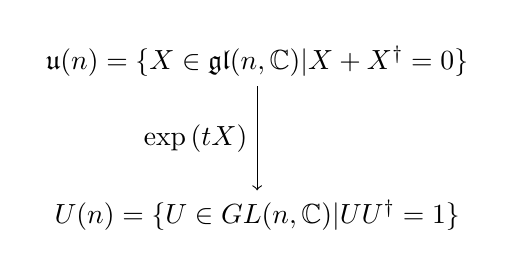
\begin{tikzpicture}
\matrix (m) [matrix of math nodes, row sep=3.8em, column sep=4.8em, minimum width=2.2em]
{
	\mathfrak{u}(n) = \lbrace X \in \mathfrak{gl}(n,\mathbb{C}) | X + X^{\dag} =0 \rbrace \\  
	U(n) = \lbrace U \in GL(n,\mathbb{C}) | UU^{\dag} = 1 \rbrace \\  
};
\path[->]
(m-1-1) edge node [left] {$\exp{(tX)}$} (m-2-1)
;
\end{tikzpicture} \quad \quad \, 
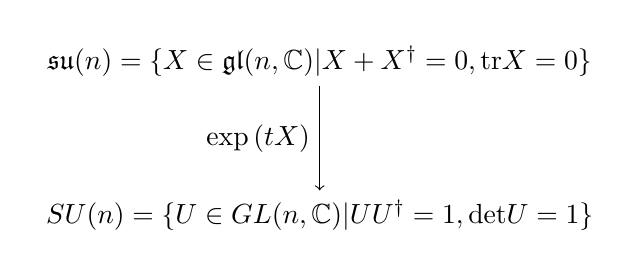
\begin{tikzpicture}
\matrix (m) [matrix of math nodes, row sep=3.8em, column sep=4.8em, minimum width=2.2em]
{
	\mathfrak{su}(n) = \lbrace X \in \mathfrak{gl}(n,\mathbb{C}) | X + X^{\dag} =0, \text{tr}{X}=0 \rbrace \\ 
	SU(n) = \lbrace U \in GL(n,\mathbb{C}) | UU^{\dag} = 1, \text{det}U=1 \rbrace \\ 
};
\path[->]
(m-1-1) edge node [left] {$\exp{(tX)}$} (m-2-1)
;
\end{tikzpicture} \\
\text{dim}_{\mathbb{R}} \mathfrak{u}(n) = n^2   \quad \quad \quad \, \text{dim}_{\mathbb{R}}\mathfrak{su}(n) = n^2-1
\end{gathered}
\]

From Chapter 5 ``Lie Groups $SU(2)$ and $SO(3)$'' of Kosmann-Schwarzbach (2010) \cite{YKosmann-Schwarzbach2010}, 

\subsubsection{Bases of $\mathfrak{su}(2)$, Subsection 1.1 of Chapter 5of Kosmann-Schwarzbach (2010) \cite{YKosmann-Schwarzbach2010}}

Recall that 

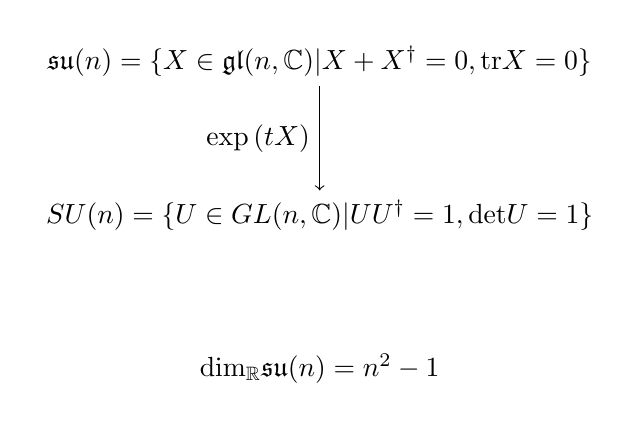
\begin{tikzpicture}
\matrix (m) [matrix of math nodes, row sep=3.8em, column sep=4.8em, minimum width=2.2em]
{
	\mathfrak{su}(n) = \lbrace X \in \mathfrak{gl}(n,\mathbb{C}) | X + X^{\dag} =0, \text{tr}{X}=0 \rbrace \\ 
	SU(n) = \lbrace U \in GL(n,\mathbb{C}) | UU^{\dag} = 1, \text{det}U=1 \rbrace \\ 
	\text{dim}_{\mathbb{R}}\mathfrak{su}(n) = n^2-1 \\
};
\path[->]
(m-1-1) edge node [left] {$\exp{(tX)}$} (m-2-1)
;
\end{tikzpicture} 

and so 

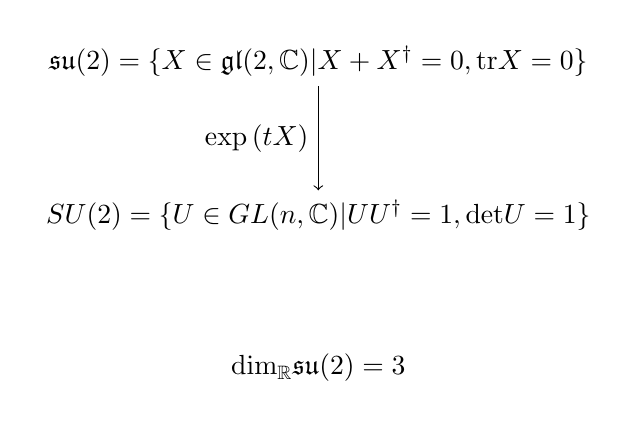
\begin{tikzpicture}
\matrix (m) [matrix of math nodes, row sep=3.8em, column sep=4.8em, minimum width=2.2em]
{
	\mathfrak{su}(2) = \lbrace X \in \mathfrak{gl}(2,\mathbb{C}) | X + X^{\dag} =0, \text{tr}{X}=0 \rbrace \\ 
	SU(2) = \lbrace U \in GL(n,\mathbb{C}) | UU^{\dag} = 1, \text{det}U=1 \rbrace \\ 
	\text{dim}_{\mathbb{R}}\mathfrak{su}(2) = 3 \\
};
\path[->]
(m-1-1) edge node [left] {$\exp{(tX)}$} (m-2-1)
;
\end{tikzpicture} 

Also, recall that $\mathfrak{g} \subseteq \mathfrak{gl}(n,\mathbb{C})$ is a vector subspace (\ref{Thm:5.1YKos}) and that \\
$X \in \mathfrak{g}$ iff $\forall t \in \mathbb{R}$, $\exp{(tX)} \in G$.  \\
if $X \in \mathfrak{g}$, if $g\in G$, then $gXg^{-1} \in \mathfrak{g}$ \\
$\mathfrak{g}$ closed under $\begin{aligned} & \quad \\
& \mathfrak{g} \times \mathfrak{g} \to \mathfrak{g} \\
& (X,Y) \mapsto [X,Y] \end{aligned}$

and so with $\mathfrak{g}$ as a vector space, we can have a choice of bases.  

\begin{enumerate}
	\item[(a)] $\begin{aligned}
	& \xi_1 = \frac{i}{2} \left( \begin{matrix} & 1 \\ 1 & \end{matrix} \right) \\ 
	& \xi_2 = \frac{1}{2} \left( \begin{matrix} & -1 \\ 1 & \end{matrix} \right) \\
	& \xi_3 = \frac{i}{2} \left( \begin{matrix} 1 &  \\  & -1 \end{matrix} \right) 
	\end{aligned}$
	
	satisfying 
	
	\[
	[\xi_k , \xi_l ] = \epsilon_{klm} \xi_m
	\]
	\item[(b)] \emph{Physics}
	
	$\begin{aligned}
	& \sigma_1 = -2i \xi_1 =  \left( \begin{matrix} & 1 \\ 1 & \end{matrix} \right) \\ 
	& \sigma_2 = 2i \xi_2 =  \left( \begin{matrix} & -i \\ i & \end{matrix} \right) \\
	& \sigma_3 = -2i \xi_3 =  \left( \begin{matrix} 1 &  \\  & -1 \end{matrix} \right) 
	\end{aligned}$
\end{enumerate}

satisfying 

\[
[ \sigma_k, \sigma_l ] = 2i \epsilon_{klm} \sigma_m
\]

EY : 20151001 Sage Math 6.8 doesn't run on Mac OSX El Capitan: I suspect that it's because in Mac OSX El Capitan, \verb|/usr| cannot be modified anymore, even in an Administrator account.  The TUG group for MacTeX had a clear, thorough, and useful (i.e. copy UNIX commands, paste, and run examples) explanation of what was going on:

\url{http://tug.org/mactex/elcapitan.html}

So keep in mind that my code for Sage Math is for Sage Math 6.8 that doesn't run on Mac OSX El Capitan.  I'll also use \verb|sympy| in Python as an alternative and in parallel.  

One can check in \verb|sympy| the traceless anti-Hermitian (or Hermitian) property of the bases and Pauli matrices, and the commutation relations (see \verb|groups.py|):

\begin{lstlisting}
import itertools
from itertools import product, permutations

import sympy
from sympy import I, LeviCivita
from sympy import Rational as Rat

from sympy.physics.matrices import msigma # <class 'sympy.matrices.dense.MutableDenseMatrix'>

def commute(A,B):
"""
commute = commute(A,B)
commute takes the commutator of A and B
"""
return (A*B - B*A)

def xi(i):
"""
xi = xi(i)
xi is a function that returns the independent basis for 
Lie algebra su(2)\equiv su(2,\mathbb{C}) of Lie group SU(2) of 
traceless anti-Hermitian matrices, based on msigma of sympy
cf. http://docs.sympy.org/dev/_modules/sympy/physics/matrices.html#msigma
"""
if i not in [1,2,3]:
raise IndexError("Invalid Pauli index")
elif i==1:
return I/Rat(2)*msigma(1)
elif i==2:
return -I/Rat(2)*msigma(2)
elif i==3:
return I/Rat(2)*msigma(3)

\end{lstlisting}

\begin{lstlisting}
## check anti-Hermitian property and commutation relations with xi 
# xi is indeed anti-Hermitian
xi(1) == -xi(1).adjoint() # True
xi(2) == -xi(2).adjoint() # True
xi(3) == -xi(3).adjoint() # True

# xi obeys the commutation relations

for i,j in product([1,2,3],repeat=2): print i,j

for i,j in product([1,2,3],repeat=2): print i,j, "\t Commutator: ", commute(xi(i),xi(j))

## check traceless Hermitian property and commutation relations with Pauli matrices
# Pauli matrices i.e. msigam is indeed traceless Hermitian

msigma(1) == msigma(1).adjoint() # True
msigma(2) == msigma(2).adjoint() # True
msigma(3) == msigma(3).adjoint() # True

msigma(1).trace() == 0 # True
msigma(2).trace() == 0 # True
msigma(3).trace() == 0 # True

# Pauli matrices obey commutation relation
print "For Pauli matrices, the commutation relations are :\n"
for i,j in product([1,2,3],repeat=2): print i,j, "\t Commutator: ", commute(msigma(i),msigma(j))

for i,j,k in permutations([1,2,3],3): print "Commute: ", i,j,k, msigma(i), msigma(j), \ 
": and is 2*i of ", msigma(k), commute(msigma(i),msigma(j)) == 2*I*msigma(k)*LeviCivita(i,j,k)

\end{lstlisting}

And finally the traceless property of the Pauli matrices:
\begin{lstlisting}
>>> msigma(1).trace()
0
>>> msigma(2).trace()
0
>>> msigma(3).trace()
0
\end{lstlisting} 

\subsection{Spin}

Let's follow the development by Baez and Muniain (1994) on pp. 175 of the Section II.1 ``Lie Groups'', the second (II) chapter on ``Symmetry'' \cite{JBaezJMuniain1994}.  

Let $V = \mathbb{C}^2$, $G=SU(2)$.  Then consider the graded algebra of polynomials on $V = \mathbb{C}^2 \ni (x,y)$
\[
\begin{gathered}
P(V) = \bigoplus_{k=0}^{\infty} P^{(k)}(V) = \bigoplus_{ \substack{ j =0 \\ 2j \in \mathbb{Z}} }^{\infty} P^{(2j)}(V) = \bigoplus_{ \substack{ j=0 \\ j\in \mathbb{Z} }}^{\infty} P^{(2j)}(V) \oplus \bigoplus_{ \substack{ j=1/2 \\ 2j \text{ odd } } }^{\infty} P^{(2j)}(V) \\
P^{(2j)}(V) \equiv \text{ vector space of complex polynomials of degree $2j$ }
\end{gathered}
\]
and recall this representation on $P^{(2j)}(V)$
\[
\begin{aligned}
& \rho^{(2j)}:G \to \text{End}(P^{(2j)}(V)) \\ 
& \rho^{(2j)}: P^{(2j)}(V) \to P^{(2j)}(V) \\ 
& \rho^{(2j)}(g)(f) = f\circ \rho(g^{-1}) \text{ where $\rho$ is the fundamental representation of $G=SU(2)$ }\\
& \rho^{(2j)}(g)(f)(v) = f\circ \rho(g^{-1})(v) \quad \, \forall \, f \in P^{(2j)}(V), \, \forall \, v \in V = \mathbb{C}^2
\end{aligned}
\]
Note, \\
$\text{dim}P^{(2j)} = \binom{2j+2-1 }{2-1} = 2j+1$

\exercisehead{21} \cite{JBaezJMuniain1994} \emph{spin-0} Consider the trivial representation $\tau$:
\[
\begin{aligned}
& \tau : G \to \text{End}(\mathbb{C}) \\ 
& \tau(g): \mathbb{C} \to \mathbb{C} \\ 
& \tau(g) = 1_{\mathbb{C}}
\end{aligned} \quad \quad \,  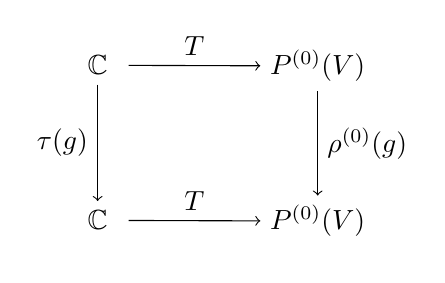
\begin{tikzpicture}
\matrix (m) [matrix of math nodes, row sep=3.8em, column sep=4.8em, minimum width=2.2em]
{
	\mathbb{C} & P^{(0)}(V) \\ 
	\mathbb{C} & P^{(0)}(V) \\ 
};
\path[->]
(m-1-1) edge node [above] {$T$} (m-1-2)
edge node [left] {$\tau(g)$} (m-2-1)
(m-1-2) edge node [auto]  {$\rho^{(0)}(g)$} (m-2-2)
(m-2-1) edge node [auto] {$T$} (m-2-2)
;
\end{tikzpicture}
\]

Clearly, $P^{(0)}(V) = \mathbb{C}$, since $P^{(0)}(V)$ consists of polynomials of constants in $\mathbb{C}$.  

Consider $c_0 \in \mathbb{C}$, $f = k_0 \in P^{(0)}(V)$ \\
$\rho^{(0)}(g)(f) = f\circ \rho(g^{-1}) = k_0$ \\
$\Longrightarrow \rho^0(g)T(c_0) = T\circ \tau(g) c_0 = T(c_0)$.  Let $T = 1_{\mathbb{C}} = 1_{P^{0}(V)}$

So $\rho^{(0)}(g) = \tau(g) = 1$.  $T=1$.  So representations $\rho^{(0)}$ and trivial representation $\tau$ on $G$ are equivalent.  



\exercisehead{22} \cite{JBaezJMuniain1994} \emph{spin-$\frac{1}{2}$} For spin-$\frac{1}{2}$, $j=\frac{1}{2}$, $2j=1$.  

$\forall \, f \in P^{(1)}(V)$, $V = \mathbb{C}^2$.  So in general form, $f(x,y) = ax + by \in P^{(1)}(V)$, $\left( \begin{matrix} x \\ y \end{matrix} \right) \in V = \mathbb{C}^2$  

Recall the fundamental representation $\begin{aligned} & \quad \\
& \rho : G \to GL(2,\mathbb{C}) \equiv GL(\mathbb{C}^2) \\
& \rho(g) : \mathbb{C}^2 \to \mathbb{C}^2 \\
& \rho(g) = g \end{aligned}$

So consider $T$ such that 

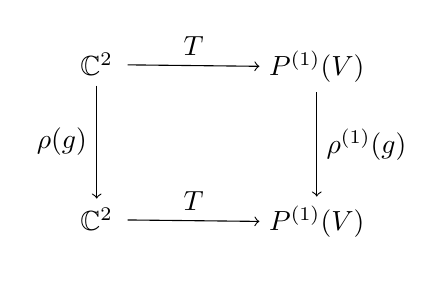
\begin{tikzpicture}
\matrix (m) [matrix of math nodes, row sep=3.8em, column sep=4.8em, minimum width=2.2em]
{
	\mathbb{C}^2 & P^{(1)}(V) \\ 
	\mathbb{C}^2 & P^{(1)}(V) \\ 
};
\path[->]
(m-1-1) edge node [above] {$T$} (m-1-2)
edge node [left] {$\rho(g)$} (m-2-1)
(m-1-2) edge node [auto]  {$\rho^{(1)}(g)$} (m-2-2)
(m-2-1) edge node [auto] {$T$} (m-2-2)
;
\end{tikzpicture}

Consider $\forall \, v \in \mathbb{C}^2$, $v =\left( \begin{matrix} x \\ y \end{matrix} \right)$, then 
\[
\rho(g)v = gv = \left[ \begin{matrix} ax + by \\ cx + dy \end{matrix} \right]
\]

\begin{lstlisting}
sage: g*X
[a*x + b*y]
[c*x + d*y]
\end{lstlisting}

For notation, let $U \in G = SU(2)$ s.t. $UU^{\dag}=1$.  

Consider $(\rho^{(2j)}(U)(f))(x) = f(U^{-1}x)$, $\forall \, x \in \mathbb{C}^2$.  

Choose $f(x,y) = x$.  So for $f(x,y) = Ax+By$, $A=1,B=0$.  Choose $U = \left( \begin{matrix} a & b \\
-\overline{b} & \overline{a} \end{matrix} \right)$ so $U^{-1} = \left( \begin{matrix} \overline{a} & -b \\
\overline{b} & a \end{matrix} \right)$.  Then $U^{-1}x = \left( \begin{matrix} \overline{a}x - by \\
\overline{b}x + ay \end{matrix} \right)$

So 
\[
\begin{aligned}
& (\rho^{(1)}(U)(f) )(x) = f(U^{-1}x) = \overline{a}x - by \\ 
& (\rho^{(1)}(U)(f))(x) = f(U^{-1}x) = \overline{b}x + ay \text{ for } f(x,y) = y 
\end{aligned}
\]
Let $f(x,y) = Ax + By$
\[
\begin{gathered}
(\rho^{(1)}(U)(f))(x) = f(U^{-1}x) = (A\overline{a}+B\overline{b})x + (Ba - Ab)y = (\overline{a}x - by)A + (\overline{b}x + ay)B  = (A\overline{a} + B\overline{b})x + (Ba-Ab)y
\end{gathered}
\]
which was calculated with the assistance of Sage Math:
\begin{lstlisting}
sage: U_try1 = Matrix( [[a.conjugate(),-b],[b.conjugate(),a ] ] )
sage: f1( U_try1*X).coefficient(x)
A*conjugate(a) + B*conjugate(b)
sage: f1( U_try1*X).coefficient(y)
B*a - A*b
\end{lstlisting}

Treating $P^{(1)}(\mathbb{C}^2)$ as a vector space, in its matrix formulation, then $f(x,y) = Ax+By \in P^{(1)}(\mathbb{C}^2)$ is treated as $\left[ \begin{matrix} A \\ B \end{matrix} \right]$, then $(\rho^{(1)}(U)f)$ is 
\[
\Longrightarrow \left[ \begin{matrix} \overline{a} & \overline{b} \\ -b & a \end{matrix} \right]\left[ \begin{matrix} A \\ B \end{matrix} \right] = \left[ \begin{matrix} A\overline{a} + B\overline{b}  \\ -Ab + Ba \end{matrix} \right]
\]
so conclude in general that $\rho^{(1)}(U) = (U^{\dag})^T$.  

Now, as Kosmann-Schwarzbach (2010) \cite{YKosmann-Schwarzbach2010} says, on pp. 13, Chapter 2 Representations of Finite Groups, ``Two representations $(E_1,\rho_1)$ and $(E_2,\rho_2)$ are equivalent if and only if there is a basis $B_1$ of $E_1$ and a basis $B_2$ of $E_2$ such that for every $g\in G$, the matrix of $\rho_1(g)$ in the basis $B_1$ is equal to the matrix of $\rho_2(g)$ in the basis $B_2$.  In particular, if the representations $(E_1,\rho_1)$ and $(E_2,\rho_2)$ are equivalent, then $E_1$ is isomorphic to $E_2$.''  So we need a change of basis between $\rho(U) = U$ and $\rho^{(1)}(U)$.  What's the linear transformation $T$ s.t.
\[
T^{-1} \rho^{(1)}(U) T = U ?
\]  
By intuition, 
\[
T = \sigma_x \sigma_z \equiv \sigma_1 \sigma_3
\]
where $\sigma_i$'s are Pauli matrices.  

Indeed, 
\begin{lstlisting}
sage: Paulimat[3] * Paulimat[1]*U_try*Paulimat[1] * Paulimat[3]
[conjugate(a) conjugate(b)]
[          -b            a]
\end{lstlisting}

Then $\rho^{(1)}(U)\circ T = TU$, so this $T = \sigma_1 \sigma_3$ is an ``intertwining operator'' between $\rho^{(1)}(U)$ and fundamental representation $\rho(U) = U$, with $T = \left[ \begin{matrix} & - 1 \\
1 & \end{matrix} \right]$, and $T^{-1} = \left[ \begin{matrix} & 1 \\ -1 & \end{matrix} \right]$.  

$T$ is an isomorphism between $\mathbb{C}^2$ and $P^{(1)}(\mathbb{C}^2)$.  So fundamental representation $\rho$ of $G=SU(2)$ is equivalent to $\rho^{(1)}(U)$ on $P^{(1)}(\mathbb{C}^2)$.  

\exercisehead{23}\cite{JBaezJMuniain1994} (Also from Exercise 2.6 of Kosmann-Schwarzbach (201) \cite{YKosmann-Schwarzbach2010})

Let $(E,\pi)$ representation of group $G$.  \\
$\forall \, g \in G$, $\xi \in E^*$, $x\in E$, set $\langle \pi^*(g)(\xi), x \rangle = \langle \xi, \pi(g^{-1})(x) \rangle$

\emph{dual} (or \emph{contragredient}) of $\pi$, $\pi^*:G \to \text{End}(E^*)$, $\pi^*$ is a representation, since
\[
\begin{gathered}
\langle \pi^*(gh)(\xi),x\rangle = \langle \xi, \pi((gh)^{-1})(x) \rangle = \langle \xi, \pi(h^{-1}g^{-1})(x) \rangle = \langle \xi, \pi(h^{-1}) \pi(g^{-1})(x) \rangle = \langle \xi, \pi(h^{-1}) (\pi(g^{-1})(x)) \rangle =  \\
= \langle \pi^*(h)(\xi), \pi(g^{-1})(x) \rangle = \langle \pi^*(g)\pi^*(h)(\xi), x \rangle
\end{gathered}
\]
since this is true, $\forall \, x \in E$, $\forall \, \xi \in E^*$, $\pi^*(gh) = \pi^*(g)\pi^*(h)$.  

dual $\pi^*$ of $\pi$ is a representation.  


\subsection{Adjoint Representation}

I will first follow Sec. 7.3 The Adjoint Representation of Ch. 4 Lie Groups and Lie Algebras of Kosmann-Schwarzbach (201) \cite{YKosmann-Schwarzbach2010}).  

The \emph{conjugation action} $\mathcal{C}_g:G\to G$ is defined as 
\[
\begin{aligned}
& \mathcal{C}_g:G\to G \\
&  \mathcal{C}_g: h \mapsto ghg^{-1}
\end{aligned}
\]
So 
\[
\begin{aligned}
& \mathcal{C}: G \to \text{Aut}(G) \\ 
& \mathcal{C}g = \mathcal{C}_g
\end{aligned}
\]
Now define the \emph{adjoint action} of $g$ as the differential or push forward of $\mathcal{C}_g$:
\[
\text{Ad}_g := D_1 \mathcal{C}_g \equiv (\mathcal{C}_g)_{*1} \equiv \left. (\mathcal{C}_g )_* \right|_{g=1}  \qquad \, (\text{adjoint action of $g$})
\]
Now $\text{Ad}_g: \mathfrak{g} \to \mathfrak{g}$, so $\begin{aligned} & \quad \\
& \text{Ad}:G \to \text{End}(\mathfrak{g}) \\
& \text{Ad}(g) \equiv \text{Ad}_g \end{aligned}$

Note $\mathcal{C}_{gg'} = \mathcal{C}_g \mathcal{C}_{g'} \equiv \mathcal{C}(gg') = \mathcal{C}(g)\circ \mathcal{C}(g')$ and so 
\[
\xrightarrow{ D_1} \text{Ad}_{gg'} = \text{Ad}_g \circ \text{Ad}_{g'}
\]

Kosmann-Schwarzbach (201) \cite{YKosmann-Schwarzbach2010}) claims, because $\text{Ad}_g = 1_{\mathfrak{g}}$ when $g=1$, 

$\begin{aligned} & \quad \\
& \text{Ad}:G \to GL(\mathfrak{g}) \\
& \text{Ad}:g\mapsto \text{Ad}_g\end{aligned}$ is a representation of $G$ on $\mathfrak{g}$.   (EY : 20160505 ???)

\begin{definition}
	representation $\text{Ad}$ of $G$ on $V=\mathfrak{g}$ is called adjoint representation of Lie group $G$.  
\end{definition}

Denote adjoint representation of Lie algebra $\mathfrak{g}$, $\text{ad}$.  

By definition, $\text{Ad}_{\text{exp}(tX)} = \exp{ (t\text{ad}_X)}$

cf. Prop. 7.8 of Kosmann-Schwarzbach (201) \cite{YKosmann-Schwarzbach2010})
\begin{proposition}
	\begin{enumerate}
		\item Let $A$ invertible matrix, $A \in $ Lie group $G$.  \\
		Let $X$ matrix s.t. $X \in \mathfrak{g}$.  Then
		\[
		\text{Ad}_A(X) = AXA^{-1}
		\]
		\item Let $X,Y \in \mathfrak{g}$.  Then 
		\[
		\text{ad}_X(Y) = [X,Y]
		\]
		\item Let $X,Y \in \mathfrak{g}$.  Then 
		\[
		\text{ad}_{[X,Y]} = [ \text{ad}_X, \text{ad}_Y ]
		\]
	\end{enumerate}
\end{proposition}
\begin{proof}
	\begin{enumerate}
		\item By def., $\forall \, B \in G$, $\mathcal{C}_A(B) = ABA^{-1}$, and thus
		\[
		\text{Ad}_A(X) = \left. \frac{d}{dt} A\exp{ (tX)  }A^{-1} \right|_{t=0} = AXA^{-1}
		\]
		\item \[
		\begin{gathered}
		\text{ad}_X(Y) = \left. \frac{d}{dt} \text{Ad}_{\exp{(tX)}}(Y) \right|_{t=0} = \left. \frac{d}{dt} \exp{(tX)} Y \exp{(tX)} \right|_{t=0} = \\
		= XY - YX = [X,Y] 
		\end{gathered}
		\]
		\item Use Jacobi identity: 
		\[
		\begin{gathered}
		[A,[B,C]] +  [B,[C,A]] +  [C,[A,B]] = 0 \text{ or } \\ 
		[[A,B],C] = [A,[B,C]] - [B,[A,C]]
		\end{gathered}
		\] 
		\[
		\begin{gathered}
		\text{ad}_{[X,Y]}C = [[X,Y],C] = [X,[Y,C]] - [Y,[X,C]] = [X,\text{ad}_YC] - [Y,\text{ad}_XC] \text{ and that } \\ 
		\text{ad}_X\text{ad}_Y C = [X,[Y,C]] \Longrightarrow \text{ad}_{[X,Y]}C = [\text{ad}_X,\text{ad}_Y ] C
		\end{gathered}
		\]
	\end{enumerate}
\end{proof}


\part{Cohomology; Stoke's Theorem}

\section{Stoke's Theorem}

\begin{theorem}[Stoke's Theorem]
	Let $M$ be oriented, smooth $n$-manifold with boundary, \\
	let $\omega$ be a compactly supported smooth $(n-1)$-form on $M$, or if $\omega \in A_c^{n-1}(M)$, \\
	Then
	\begin{equation}
	\int_M d\omega = \int_{\partial M} \omega
	\end{equation} 
	If $\partial M = \emptyset$, then $\int_{\partial M} \omega = 0$
	
	$\int_{\partial M} \omega$ interpreted as $\int_{\partial M} i^*_{\partial M} \omega = \int_{\partial M} i^*\omega$ so 
	\begin{equation}
	\int_M d\omega = \int_{\partial M} i^*(\omega)
	\end{equation}
	where inclusion $i: \partial M \hookrightarrow M$
\end{theorem}

\begin{proof}
Begin with very special case: \\
Suppose $M = \mathbb{H}^n$ (upper half space), $\partial M = \mathbb{R}^{n-1}$ \\
$\omega$ has compact support, so $\exists \, R >0$ s.t. $\text{supp}\omega \subseteq $ rectangle $A=[-R,R] \times \dots \times [-R, R] \times [0,R]$.  

$\forall \, \omega \in A_c^{n-1}(\mathbb{H}^n)$
\begin{equation}
\omega = \sum_{j=1}^n (-1)^{j-1} f_j dx^1 \wedge \dots \wedge \widehat{dx}^j \wedge \dots \wedge dx^n \equiv \sum_{i=1}^n \omega_i dx^1 \wedge \dots \wedge \widehat{dx}^i \wedge \dots \wedge dx^n
\end{equation}
with Conlon (2008) \cite{Conl2008} and John Lee (2012) \cite{JLee2012}'s notation, respectively, and where $f_j$ has compact support.  

\[
i^*\omega = (f_1 \circ i) dx^2 \wedge \dots \wedge dx^n \in A_c^{n-1}(\partial \mathbb{H}^n)
\]
\[ 
\begin{aligned}
d\omega & = \sum_{i=1}^n d\omega_i \wedge dx^1 \wedge \dots \wedge \widehat{dx}^i \wedge \dots \wedge dx^n = \sum_{i,j=1}^n \frac{\partial \omega_i}{ \partial x^j} dx^j \wedge dx^1 \wedge \dots \wedge \widehat{dx}^i \wedge \dots \wedge dx^n = \\
& = \sum_{i=1}^n (-1)^{i-1} \frac{ \partial \omega_i}{ \partial x^i } dx^1 \wedge \dots \wedge dx^n
\end{aligned}
\]
i.e. (for another notation)
\[
d\omega = \left( \sum_{j=1}^n \frac{\partial f_j}{ \partial x^j} \right) dx^1 \wedge \dots \wedge dx^n \in A_c^n(\mathbb{H}^n)
\]

\[
d\omega = \left( \sum_{j=1}^n \frac{\partial f_j}{ \partial x^j} \right) dx^1 \wedge \dots \wedge dx^n \in A_c^n(\mathbb{H}^n)
\]

\[
\int_{\mathbb{H}^n} d\omega = \sum_{i=1}^n (-1)^{i-1} \int_A \frac{ \partial \omega_i}{ \partial x^i } dx^1 \wedge \dots \wedge dx^n = \sum_{i=1}^n (-1)^{i-1} \int_0^R \int_{-R}^R \dots \int_{-R}^R dx^1 \dots dx^n \frac{ \partial \omega_i}{\partial x^i}(x)
\]

We can change order of integration in each term so to do $x^i$ integration first. 

By fundamental thm. of calculus, terms for which $i\neq n$ reduce to 
\[
\begin{gathered}
\sum_{i=1}^{n-1} (-1)^{i-1} \int_0^R \int_{-R}^R \dots \int_{-R}^R \frac{\partial \omega_i}{\partial x^i}(x) dx^1 \dots dx^n = \sum_{i=1}^{n-1} (-1)^{i-1} \int_0^R \int_{-R}^R \dots \int_{-R}^R \frac{\partial \omega_i}{\partial x^i}(x) dx^i dx^1 \dots \widehat{dx}^i \dots dx^n = \\
= \sum_{i=1}^{n-1} (-1)^{i-1} \int_0^R \int_{-R}^R \dots \int_{-R}^R [\omega_i(x)]_{x^i = -R}^{x^i = R} dx^1 \dots \widehat{dx}^i \dots dx^n = 0 
\end{gathered} 
\]
because we've chosen $R$ large enough that $\omega =0 $ when $x^i = \pm R$.  
	
	
\end{proof}

\part{Pr\'{a}staro}

Pr\'{a}staro (1996) \cite{Pras1996}

\subsubsection{Affine Spaces}

cf. Sec. 1.2 - \emph{Affine Spaces} of Pr\'{a}staro (1996) \cite{Pras1996}

\begin{definition}[affine space]
  \begin{equation}
\begin{gathered}
    \text{ affine space \qquad \, } (M, \mathbf{M}, \alpha )  \\
    \text{ with } \\
    \begin{aligned}
      & M \equiv \text{ set (set of pts.) }  \\ 
      & \mathbf{M} \equiv \text{ vector space (space of free vectors) } \\
      & \alpha \equiv \mathbf{M} \times M \to M \equiv \text{ translation operator } \\
      & \alpha : (v,p ) \mapsto p' \equiv p + v
      \end{aligned}
\end{gathered}
  \end{equation}
  Note: $\alpha$ is a \textbf{transitive} action and without fixed pts. (free).

  i.e. $\forall \, p \in M$, 
  \end{definition}

$\forall \, $ pt. $O \in M$, $\alpha:(v,O) \mapsto O' \equiv O + v$, $\alpha (\cdot , O) \equiv \alpha_O \equiv \alpha(O)$.  $\alpha_O(v) = O' = O + \mathbf{v}$ \qquad \, $\forall \, O' \in M$, $\exists \, \mathbf{v} \in \mathbf{M}$ s.t. $O' = O + \mathbf{v}$ \\
$\Longrightarrow M \equiv \mathbf{M}$.

$\forall \, (O, \lbrace e_i \rbrace)_{1 \leq i \leq n }$, where $\lbrace e_i \rbrace$ basis of $\mathbf{M}$, $M \equiv \mathbf{M} = \mathbb{R}^n$ so isomorphism $M \simeq \mathbb{R}^n$ \\

i.e. $\alpha$ is \textbf{without fixed pts.}, meaning, 

Given pointed space $(M, O)$, where base pt. $O\in M$, we can associate $\forall \, p \in M$, vector $\mathbf{x} \in \mathbf{M}$, by 1-to-1 mapping $M\to \mathbf{M}$. 

So for 
\[
\begin{aligned}
& \alpha : \mathbf{M} \times M \to M \\ 
& \alpha(\mathbf{x}, p) = p' = p + \mathbf{x}
\end{aligned}
\]
Consider 
\[
\begin{gathered}
	\alpha(\mathbf{x}, O) = p = \alpha_O(\mathbf{x}) = p \Longrightarrow \exists \, \alpha_O^{-1}(p) = \mathbf{x} \in \mathbf{M}
\end{gathered}
\]

\begin{enumerate}
	\item tangent space of $M$ in $p\in M$ is vector space $T_pM \equiv (\mathbf{M}, p) \cong M$
	\item If $\mathbf{M}$ Euclidean space, affine space $(M, \mathbf{M}, \alpha)$ is Euclidean
	\item Call dim. of affine space $(M, \mathbf{M}, \alpha)$, dim. of $\mathbf{M} \equiv \text{dim}{\mathbf{M}}$
\end{enumerate}
$\lbrace \mathbf{e}_i \rbrace$ basis of $\mathbf{M}$




\begin{definition}
  $(O, \lbrace e_i \rbrace) \equiv $ affine frame.

  $\forall \, $ affine frame $(O,\lbrace e_i \rbrace)$, $\exists \, $ coordinate system $x^{\alpha} : M \to \mathbb{R}$, \\
  where $x^{\alpha}(p)$ is $\alpha$th component, in basis $\lbrace e_i \rbrace$, of vector $p-O$
  \end{definition}

\begin{proposition}[1.6, Pr\'{a}staro (1996) \cite{Pras1996}]
	$\forall \, O \in M$, we have canonical identification $M \equiv \mathbf{M}$, since
	\[
	\begin{gathered}
	\begin{aligned}
	& \alpha^{-1}_O:M \to \mathbf{M} \\
	& \alpha^{-1}_O(p) = \mathbf{x} 
	\end{aligned} \qquad \quad \, 
	\begin{aligned}
	& \alpha_O : \mathbf{M} \to M \\
	& \alpha_O: \mathbf{x} = \alpha(\mathbf{x}, O) = p
	\end{aligned}
	\end{gathered}
	\]
	Furthermore, \\
	$\forall \, $ \textbf{affine frame} $(O, \lbrace \mathbf{e}_i \rbrace)_{1\leq i \leq d}$, where $\lbrace \mathbf{e}_i \rbrace$ basis of $\mathbf{M}$, \\
	\phantom{Furthermore} $\exists \, $ isomorphism $M \cong \mathbb{R}^d$, \\
	Then, $\forall \, (O, \lbrace \mathbf{e}_i \rbrace)_{1 \leq i \leq d}$, \\
	\phantom{Then} $\exists \, $ coordinate system $x^{\alpha} : M \to \mathbb{R}$, \\
	\phantom{Then $\exists \, $} where $x^{\alpha}(p) = \alpha$th component, in basis $\lbrace \mathbf{e}_i \rbrace$, of vector $p - O$. 
	
	
	
\end{proposition}

\begin{theorem}[1.4 Pr\'{a}staro (1996) \cite{Pras1996}]
  Let $(x^{\alpha}), (\overline{a}^{\alpha})$ 2 coordinate systems correspond to affine frames $(O, \lbrace e_i \rbrace)$, $( \overline{O}, \lbrace \overline{e}_i \rbrace )$, respectively.
\begin{equation}
  \overline{x}^{\alpha} = A^{\alpha}_{ \, \, \beta} x^{\beta} + y^{\alpha}
\end{equation}
where
\[
y^{\alpha} \in \mathbb{R}^n, \qquad \, A^{\alpha}_{ \, \, \beta} \in GL(n; \mathbb{R})
\]
\end{theorem}

\begin{definition}[1.10 Pr\'{a}staro (1996) \cite{Pras1996}]
  \begin{equation}
    A(n) \equiv Gl(n,\mathbb{R}) \times \mathbb{R}^n
  \end{equation}
  affine group of dim. $n$
  \end{definition}

\begin{theorem}[1.5] symmetry group of $n$-dim. affine space, called affine group $A(M)$ of $M$.  $\exists \, $ isomoprhism,
  \begin{equation}
    A(M) \simeq A(n), \qquad \, f\mapsto (f^{\alpha}_{ \, \, \beta} , y^{\alpha}) \, ; \qquad \, f^{\alpha} \equiv x^{\alpha} \circ f = f^{\alpha}_{ \, \, \beta} x^{\beta} + y^{\alpha}
  \end{equation}
cf. Eq. 1.4 Pr\'{a}staro (1996) \cite{Pras1996}
  \end{theorem}

\begin{definition}[metric]
	Let smooth manifold $M$, $\text{dim}M = n$, $\forall \, p \in M$, $\exists \, $ vector space $T_pM$, and so for 
	\begin{equation}
	\begin{aligned}
	& g_p (T_pM)^2 \to \mathbb{R} \\
	& g_p : (X_p,Y_p) \mapsto g_p(X_p,Y_p) \in \mathbb{R}
	\end{aligned}
	\end{equation}
	with $g_p$ being bilinear, symmetric (in $X_p,Y_p$), nondegenerate (i.e. if $g_p(X_p,Y_p)=0$, then $X_p$ or $Y_p=0$)
	
	Note that 
	\[
	g\in \Gamma((TM \otimes TM)^*)
	\]
	and that for $\begin{aligned} & \quad \\ 
	& X = X^i \frac{ \partial }{ \partial x^i } \\
	& Y = Y^i \frac{ \partial }{ \partial x^i } \end{aligned}$  
	so 	
	\[
	g(X,Y) = g_{ij} X^i Y^j
	\]  
	
\end{definition}

Now for 
\[
\begin{gathered}
\begin{aligned} 
& F: M \to N \\
& F: x \mapsto y = y(x) 
\end{aligned} \qquad \, \begin{aligned}
& DF \equiv F_* : T_p M \to T_{F(p)}N \\ 
&  DF : X_p \mapsto (DF) (X^j \frac{ \partial }{ \partial x^j }) = X^j \frac{\partial y^i}{\partial x^j} \frac{ \partial }{ \partial y^i}
\end{aligned}
\end{gathered}
\]
\[
\begin{gathered}
(F^* g')(X,Y) = (F^*g')(X^i \frac{ \partial }{ \partial x^i } , Y^j \frac{ \partial }{ \partial x^j} ) = (F^*g')_{ij} X^i Y^j = g'(F_*X, F_*Y) = \\
= 
\end{gathered}
\]





\part{Holonomy}

\begin{definition}[Conlon, 10.1.2] If $X,Y\in \mathfrak{X}(M)$, $M\subset \mathbb{R}^m$, \textbf{Levi-Civita connection} on $M\subset \mathbb{R}^m$
	\begin{equation}
	\begin{aligned}
	& \nabla : \mathfrak{X}(M) : \mathfrak{X}(M) \to \mathfrak{X}(M) \\
	\nabla_XY := p(D_XY)
	\end{aligned}
	\end{equation}
	with 
	\[
	D_XY := \sum_{j=1}^m X(Y^j) \frac{ \partial }{ \partial x^j} = \sum_{i,j=1}^m X^i \frac{ \partial Y^j}{ \partial x^i} \frac{ \partial }{ \partial x^j} \qquad \,  \begin{aligned} & \quad \\ 
		& \forall \, X=\sum_{i=1}^m X^i \frac{ \partial }{ \partial x^i},  \\
		& \forall \, Y=\sum_{i=1}^m Y^i \frac{\partial }{ \partial x^i } \end{aligned}
	\]
\end{definition}

\[
\begin{aligned}
	& \nabla_{fX}Y = f(D_{fX}Y) = p(fD_XY) = fpD_XY = f\nabla_XY \\ 
	&  \nabla_X fY = p(D_XfY) = p \left( \sum_{i,j=1}^m \left( X^i f\frac{ \partial Y^j}{ dx^i } + X^i Y^j \frac{ \partial f}{ \partial x^i} \right) \frac{ \partial }{ \partial x^j} \right) = f\nabla_X Y + p \sum_{j=1}^m X(f) Y^j \frac{ \partial }{ \partial x^j} = f\nabla_XY + X(f) p(Y)
\end{aligned}
\]


\begin{definition}[Conlon, 10.1.4; Christoffel symbols] 
\begin{equation}
\begin{gathered}
	\nabla_{\frac{ \partial }{ \partial x^i} \frac{ \partial }{ \partial x^j} = \Gamma^k_{ij} \frac{ \partial }{ \partial x^k} \qquad \, \text{ (Conlon's notation) }  }   \\
	\nabla_{\frac{ \partial }{ \partial x^j} \frac{ \partial }{ \partial x^i} = \Gamma^k_{ij} \frac{ \partial }{ \partial x^k} \qquad \, \text{ (F. Schuller's notation) }  }
\end{gathered}
\end{equation}
\end{definition}





\begin{definition}[torsion]
\begin{equation}
\begin{aligned}
	& T:\mathfrak{X}(M) \in \mathfrak{X}(M) \to \mathfrak{X}(M) \\ 
	& T(X,Y) = \nabla_XY - \nabla_Y X - [X,Y] 
\end{aligned}
\end{equation}
If $T=0$, $\nabla$ torsion-free or symmetric.  
\end{definition}
\[
\begin{gathered}
T(fX,Y) = f\nabla_XY - (f\nabla_Y X + Y(f)X) - \lbrace (fXY - (Y(f)X + fYX) \rbrace = fT(X,Y) \\ 
T(X,fY) = f\nabla_XY + X(f)Y - f\nabla_Y X   - \lbrace ( ( X(f) Y +fXY) -  fYX \rbrace = fT(X,Y)  
\end{gathered}
\]
Thus, $T(X,Y)$ $C^{\infty}(M)$-bilinear.  

$T\in \tau_1^2 (M)$.  

$T(v,w) \in T_xM$ defined, $\forall \, v,w \in T_xM$, $\forall \, x\in M$.

Thus, torsion is a \textbf{tensor}.

\exercisehead{10.1.7 Conlon (2008)\cite{Conl2008} }.  

If $T(X,Y)=0$,
\[
T(e_i,e_j) = \Gamma^k_{ji} e_k - \Gamma^k_{ij} e_k - 0 = 0 \Longrightarrow \Gamma_{ji}^k = \Gamma^k_{ij}
\]

If $\Gamma^k_{ij} = \Gamma^k_{ji}$, $T(e_i,e_j)=0$.  

\exercisehead{10.1.8, Conlon (2008)\cite{Conl2008}} 

If $M\subset \mathbb{R}^m$ smoothly embedded submanifold,  
$\forall \, \frac{ \partial }{ \partial x^j}, \frac{ \partial }{ \partial x^i} \in T_xM$, spanning $T_xM$, consider $\frac{ \partial }{ \partial x^j} = X^k_j \frac{ \partial }{ \partial \widetilde{x}^k}$, $\frac{ \partial }{ \partial x^i} = X_i^k(\widetilde{x}) \frac{ \partial }{ \partial \widetilde{x}^k}$  

\[
\begin{gathered}
	\nabla_{\frac{\partial }{ \partial x^j} } \frac{ \partial }{ \partial x^i} = p D_{ X^k_j \frac{ \partial }{ \partial \widetilde{x}^k } } X^l_i \frac{ \partial }{ \partial \widetilde{x}^l } = p \left( X^k_j \frac{ \partial X^l_i}{  \partial \widetilde{x}^k } \frac{ \partial }{ \partial \widetilde{x}^l } \right) =   X^k_j  p \left( \frac{ \partial X^l_i}{  \partial \widetilde{x}^k } \frac{ \partial }{ \partial \widetilde{x}^l } \right)  \\ 
	\nabla_{\frac{\partial }{ \partial x^i} } \frac{ \partial }{ \partial x^j} =  X^k_i p \left(  \frac{ \partial X^l_j }{ \partial \widetilde{x}^k }   \frac{ \partial }{ \partial \widetilde{x}^l  } \right) 
\end{gathered}
\]









If $X\in \mathfrak{X}(M)$, smooth $s:[a,b]\to M$, 

then $\forall \, s(t)$, 
\[
X'_{s(t)} = \nabla_{\dot{s}(t)} X \in T_{s(t)}M
\]
In fact, it's often natural to consider fields $X_{s(t)}$ along $s$, parametrized by parameter $t$, allowing
\[
X_{s(t_1)} \neq X_{s(t_2)}
\]
each of $s(t_1)=s(t_2)$.  

\begin{definition}[10.1.9] Let smooth $s:[a,b] \to M$.  

Vector field along $s$ is smooth $v:[a,b]\to TM$ s.t. 
\[
\begin{tikzpicture}
  \matrix (m) [matrix of math nodes, row sep=7.8em, column sep=12.8em, minimum width=5.2em]
  {
   &  TM  \\ 
	\left[ a,b \right] & M \\ 
};
  \path[|->]
  (m-2-1) edge node [above] {$ v $} (m-1-2)
edge node [above] {$s$} (m-2-2)
  (m-1-2) edge node [left] {$ \pi $} (m-2-2)
  ;
\end{tikzpicture}  
\]
commutes.

Note that $v\in \mathfrak{X}(s) \subset \mathfrak{X}(M)$
\end{definition}

e.g. $(Y|s)(t) = Y_{s(t)}$, restriction of $Y\in \mathfrak{X}(M) $ to $s$.  

e.g. $\dot{s}(t) \in \mathfrak{X}(M)$.  

$\forall \, v,w \in \mathfrak{X}(s)$, $v+w \in \mathfrak{X}(s)$, 
\[
\begin{gathered}
	(fv+gv)(t) := (f(s(t)) + g(s(t)) )v(t) = f(s(t)) v(t) + g(s(t)) v(t) = (f+g)v(t)
\end{gathered}
\]
Likewise, 
\[
f(v+w) = fv+fw
\]
$\mathfrak{X}(s)$ is a real vector space and $C^{\infty}[a,b]$-module.  

\begin{definition}[10.1.10]
Let conection $\nabla$ on $M$.  

\textbf{Associated covariant derivative} is operator 
\[
\frac{\nabla}{dt} \mathfrak{X}(s) \to \mathfrak{X}(s)
\]
$\forall \, $ smooth $s$ on $M$, s.t. 
\begin{enumerate}
\item $\frac{\nabla}{dt}$ $\mathbb{R}$-linear 
\item $\left( \frac{\nabla}{dt} \right)(fv) = \frac{df}{dt} v+ f\frac{\nabla}{dt} v$, $\forall \, f \in C^{\infty}[a,b]$, $\forall \, v\in \mathfrak{X}(s)$  
\item If $Y\in \mathfrak{X}(M)$, then
\[
\frac{\nabla}{dt} (Y|s)(t) = \nabla_{ \dot{s}(t)}Y \in T_{s(t)} M, \quad \, a\leq t \leq b
\]
\end{enumerate}
\end{definition}












\begin{theorem}[Conlon Thm. 10.1.11\cite{Conl2008} ]
	$\forall \, $ connection $\nabla$ on $M$, $\exists \, !$ \, associated covariant derivative $\frac{ \nabla }{dt}$
\end{theorem}

\begin{proof}
	Consider arbitrary coordinate chart $(U,x^1 \dots x^n)$.  
	
	Consider smooth curve $s:[a,b]\to U$.  
	
	Let $v\in \mathfrak{X}(s)$, $v(t) = v^i(t) \frac{ \partial }{ \partial x^i}$; $\dot{s}(t) = s^j \frac{ \partial }{ \partial x^j}$.  
	\[
	\begin{gathered}
	\frac{ \nabla v}{ dt} = \frac{dv^i(t) }{dt}\frac{ \partial }{ \partial x^i} + v^i(t) \frac{ \nabla}{dt} \frac{ \partial }{ \partial x^i} = \frac{ d v^i }{dt}	\frac{ \partial }{ \partial x^i} + v^i \nabla_{ \dot{s}(t) } \frac{ \partial }{ \partial x^i } = \dot{v}^i \frac{ \partial }{ \partial x^i } + v^i\dot{s}^j \Gamma^k_{ij} \frac{ \partial }{ \partial x^k} = \left( \dot{v}^k + v^i \dot{s}^j \Gamma^k_{ij} \right)\frac{ \partial }{ \partial x^k} \end{gathered}
	\]
	This is an explicit, local formula in terms of connection, proving uniqueness.  
	
	Existence: $\forall \, $ coordinate chart $(U,x^1\dots x^n)$, $\left( \dot{v}^k + v^i \dot{s}^j \Gamma_{ij}^k \right) \frac{ \partial }{ \partial x^k } =: \frac{ \nabla v}{dt}$.  
	
	\[
	\begin{gathered}
	\frac{\nabla}{dt}(fv) = \dot{f}v^k + f\dot{v}^k + fv^i \dot{s}^j = \dot{f}v + f\frac{ \nabla v}{dt}
	\end{gathered}
	\]
If $f$ constant, then $\frac{\nabla}{dt}$ is $\mathbb{R}$-linear.  	

\end{proof}

\begin{definition}[10.1.12 Conlon (2008)\cite{Conl2008}]
	Let $(M,\nabla)$.  Let $v\in\mathfrak{X}(s)$ for smooth $s:[a,b] \to M$.  

If $\frac{\nabla v}{dt} \equiv 0$ on $s$, then $v$ is \textbf{parallel } along $s$.  
\end{definition}

\begin{theorem}[10.1.13] 
Let $(M,\nabla)$, smooth $s:[a,b]\to M$, $c\in [a,b]$, $v_0 \in T_{s(c)}M$.  

Then $\exists \, !$ parallel field $v\in \mathfrak{X}(s)$ s.t. $v(c) = v_0$.  

$v$ parallel transport along $s$.  
\end{theorem}
\begin{proof}
	\[
\begin{aligned}
	& \dot{s}(t) = \dot{s}^j(t) e_j \\ 
	&  v(t) = v^i(t) e_i  \\
& v_0 = a^i e_i
\end{aligned}
\]
\[
0 = \left( \frac{dv^k}{dt}(t) + v^i(t) \dot{s}^j(t) \Gamma^k_{ij}(s(t)) \right) e_k
\]
or equivalently
\begin{equation}
	\frac{dv^k}{dt} = - v^i \dot{s}^j \Gamma^k_{ij} , \qquad \, 1\leq k \leq n \qquad \, (10.1)
\end{equation}
with initial conditions $v^k(c) = a^k$, $1\leq k \leq n$.  

By existence and uniqueness of solutions of O.D.E.  

$\exists \, \epsilon > 0$ s.t. $\exists \, !$ solutions $v^k(t)$.  For $c-\epsilon < t < c+\epsilon$.  

In fact, these ODEs being linear in $v^k$,  by ODE theory (Appendix C, Thm. C.4.1).  

$\nexists \, $ restriction on $\epsilon$, so $\exists \, ! \, v^k(t)$ \, $\forall \, t \in [a,b]$, $1\leq k \leq n$  

\end{proof}




\subsubsection{Principal bundle, vector bundle case for parallel transport}  

Recall the 2 different forms or viewpoints for Lie-algebra valued 1-forms, or vector-valued 1-forms, or sections of 1-form-valued endomorphisms:
\[
\omega^k_{ \,\, i\mu} dx^{\mu} \equiv \omega^k_{\,\,i} \in \Omega^1(M,\mathfrak{gl}(n,\mathbb{F})) = \Gamma(\mathfrak{gl}(n,\mathbb{R} \otimes \left. T^* M \right|_U ) )
\] 
for $\begin{aligned} & \quad \\
	& i,k = 1\dots n =\text{dim}E \\ 
	& \mu = 1\dots d =\text{dim}E \end{aligned}$.  

Now
\[
D_X\mu = X^{\mu} D_{\frac{\partial }{ \partial x^{\mu}}}\mu = X^{\mu} \left[ \left( \frac{ \partial }{ \partial x^{\mu}} \mu^k \right) e_k + \mu^i \omega^k_{ \,\, i\mu} e_k \right] = \left( X(\mu^k) + \mu^i \omega^k_{ \,\, i}(X) \right) e_k = \left( d\mu^k(X) + \mu^i \omega^k_{ \,\, i}(X) \right) e_k
\]
So then define 
\begin{equation}
	\begin{aligned}
		& D: \Gamma(E) \to \Gamma(E) \otimes \Gamma(T^*M) \\
	& D\mu  = D(\mu^i e_i) = e_k ( d\mu^k +\mu^i \omega^k_{ \,\, i}) \equiv (d+A)\mu
	\end{aligned}
\end{equation}

Also, $D$ can be defined for this case:
\[
D: \Gamma (\text{End}(E)) \to \Gamma(\text{End}E) \otimes \Gamma(T^*M)
\]
Let $\sigma = \sigma^i_{ \,\, j} e_i \otimes e^j \in \Gamma(\text{End}(E))$

\begin{equation}
\begin{gathered}
	D\sigma = D(\sigma^i_{ \,\, j} e_i ) \otimes e^j + \sigma^i_{ \,\, j} e_i \otimes D^* e^j = \left( d\sigma^k_{ \,\, j} + \sigma^i A^k_{ \,\, i} \right) e_k \otimes e^j + \sigma^i_{ \,\, j} e_i \otimes (A^*)_k^{ \,\, j} e^k = \\
	= (d\sigma^k_{ \,\, j} + \sigma^i_{ \,\, j} A^k_{ \,\, i} ) e_k \otimes e^j + \sigma^k_{ \,\, i} e_j \otimes (- A^i_{ \, \, j}) e^j = (d\sigma^k_{ \,\, j} + [A,\sigma]^k_{ \,\, j}) e_k\otimes e^j
\end{gathered}
\end{equation}
cf. Def. 4.1.4 of Jost (2011), pp. 138.  

For $\mu \in \Gamma(E)$, smooth $s:[a,b] \to M$, $X(t) = \dot{s}(t)$,
\begin{equation}
D_{\dot{s}(t)}\mu = \dot{s}^{\mu}D_{\frac{ \partial }{ \partial x^{\mu}} } \mu = \dot{s}^{\mu} \left[ \frac{ \partial \mu^k }{ \partial x^{\mu}} e_k + \mu^i \omega^k_{ \, \, i\mu} e_k \right] = \left[ \dot{s}^{\mu} \frac{ \partial \mu^k}{ \partial x^{\mu} } + \dot{s}^{\mu} \mu^i \omega^k_{ \,\, i \mu} \right] e_k =\frac{d}{dt} \mu(s(t)) + \mu^i \dot{s}^{\mu} \omega^k_{ \,\, i \mu} e_k
\end{equation}

Let $D_{\dot{s}(t)}\mu=0$.  Then, 
\begin{equation}
\frac{d}{dt} \mu(s(t)) = -\mu^i \dot{s}^{\mu}\omega^k_{ \,\, i\mu} e_k
\end{equation}


Recall, given vector bundle $E\xrightarrow{ \pi} N$, given $\varphi : M\to N$, then pullback 
\begin{equation}
	\varphi^* E \to M
\end{equation}
i.e. 

\[
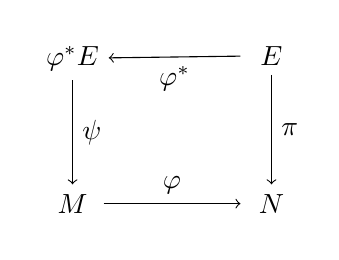
\begin{tikzpicture}
\matrix (m) [matrix of math nodes, row sep=3.8em, column sep=4.8em, minimum width=2.2em]
{
	\varphi^* E &  E  \\
	M  &  N  \\
};
\path[->]
(m-1-2) edge node [auto] {$ \varphi^*  $} (m-1-1)
edge node [auto] {$ \pi $} (m-2-2)
(m-2-1) edge node [auto]  {$  \varphi $} (m-2-2)
(m-1-1) edge node [auto] {$\psi$} (m-2-1)
;
\end{tikzpicture}
\qquad \, 
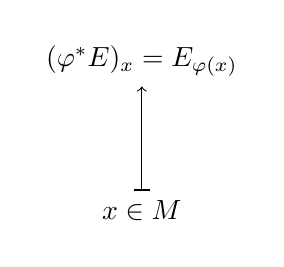
\begin{tikzpicture}
\matrix (m) [matrix of math nodes, row sep=3.8em, column sep=4.8em, minimum width=2.2em]
{
	(\varphi^* E)_x = E_{\varphi(x)}  \\
	 x\in M \\
};
 \path[|->]
	(m-2-1) edge node [auto] {$$} (m-1-1)
;
\end{tikzpicture}
\]
i.e. if $s\in \Gamma(E)$, 
\[
\varphi^* s = s \circ \varphi \in \Gamma( \varphi^* E)
\]
Thus,
\[
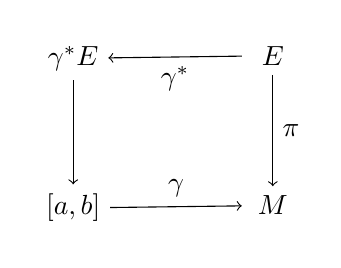
\begin{tikzpicture}
\matrix (m) [matrix of math nodes, row sep=3.8em, column sep=4.8em, minimum width=2.2em]
{
	\gamma^* E &  E  \\
	\left[a,b\right]  &  M  \\
};
\path[->]
(m-1-2) edge node [auto] {$ \gamma^*  $} (m-1-1)
edge node [auto] {$ \pi $} (m-2-2)
(m-2-1) edge node [auto]  {$  \gamma $} (m-2-2)
(m-1-1) edge node [auto] {$ $} (m-2-1)
;
\end{tikzpicture}
\qquad \, 
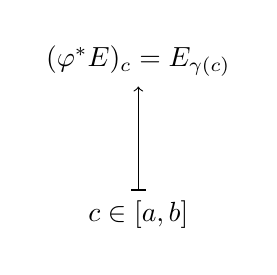
\begin{tikzpicture}
\matrix (m) [matrix of math nodes, row sep=3.8em, column sep=4.8em, minimum width=2.2em]
{
	(\varphi^* E)_c = E_{\gamma(c)}  \\
	 c\in  [a,b]\\
};
 \path[|->]
	(m-2-1) edge node [auto] {$$} (m-1-1)
;
\end{tikzpicture}
\]







For 
\[
\begin{gathered}
\dot{v}^k = -v^i \dot{s}^j \Gamma^k_{ \, \, ij}   \\
v^k(c) = v_0^k \qquad \, 1 \leq k \leq m
\end{gathered}
\]
\[
\dot{v} = -v^i \dot{s}^j \Gamma_{ij}
\]
\[
\begin{gathered}
\dot{ (v+w) } = -(v^i + w^i) \dot{s}^j \Gamma_{ij}
(v+w)(c) = v(c) + w(c) = v_0 + w_0 
\end{gathered}
\]
so $v+w\in \mathfrak{X}(s)$ is parallel transport of $v_0 + w_0$.  

Likewise, $\forall \, a \in \mathbb{F}$, $av \in \mathfrak{X}(s)$ is the parallel transport of $av_0$.  

\[
\dot{\mu}^k = - \mu^i \dot{s}^{\mu} \omega^k_{ \, \, i \mu} = -\mu^i \omega^k_{ \,\, i}(\dot{s}^{\mu})
\]


Suppose $\gamma^*E$ trivialized over $[a,b]$.  

Closed interval is contractible, so this is always possible.  

For chart $(U,\varphi)$, 
\[
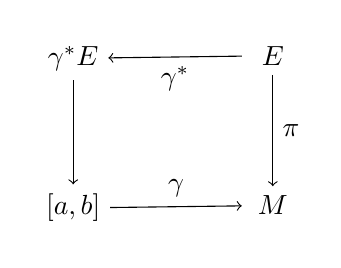
\begin{tikzpicture}
\matrix (m) [matrix of math nodes, row sep=3.8em, column sep=4.8em, minimum width=2.2em]
{
	\gamma^* E   &  E    \\
	\left[a,b\right]  &  M  \\
};
\path[->]
(m-1-2) edge node [auto] {$ \gamma^*  $} (m-1-1)
edge node [auto] {$ \pi $} (m-2-2)
(m-2-1) edge node [auto]  {$  \gamma $} (m-2-2)
(m-1-1) edge node [auto] {$ $} (m-2-1)
;
\end{tikzpicture} \qquad \, 
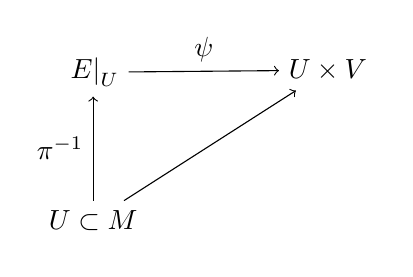
\begin{tikzpicture}
\matrix (m) [matrix of math nodes, row sep=3.8em, column sep=4.8em, minimum width=2.2em]
{
	\left. E \right|_U   &   U\times V  \\
	U \subset M    &    \\
};
\path[->]
(m-2-1) edge node [auto] {$ \pi^{-1}  $} (m-1-1)
edge node [auto] {$  $} (m-1-2)
(m-1-1) edge node [auto]  {$  \psi $} (m-1-2)
%(m-1-1) edge node [auto] {$ $} (m-2-1)
;
\end{tikzpicture}
\]
Consider 
\[
\begin{aligned}
& \varphi:[a,b]  \times V \to \gamma^* E \\ 
& \varphi(t,\cdot ) = \gamma^* \circ \psi^{-1}(\gamma(t), \cdot ) 
\end{aligned}
\]
$\forall \, \mu \in \Gamma( \left. E\right|_{x\in M} )$, \\ 
$\mu = \mu^i e_i$.  

$\varphi(t,e_i) = \epsilon_i$ is a basis for $\gamma^* E$.  

$\forall \, \sigma \in \Gamma(\gamma^*E)$,  
\[
\sigma  = \sigma^i \epsilon_i, \quad \, \sigma^i: [a,b] \to \mathbb{F}
\]
\[
\begin{gathered}
	\nabla_{ \frac{ \partial }{ \partial x^{\mu} } } \sigma = \frac{ \partial \sigma^k}{ \partial x^{\mu}  } \epsilon_k + \omega^k_{ \, \, j \mu } \sigma^j \epsilon_k = \left( \frac{ \partial \sigma ^k }{ \partial x^{\mu } } + \omega^k_{ \ , \, j \mu} \sigma^j  \right)  \epsilon_k \\ 
 \nabla \sigma = \epsilon_k \otimes ( d\sigma^k + \omega^k_{ \, \, j \mu} dx^{\mu} \sigma^j ) = \epsilon_k \otimes (d\sigma^k + \omega^k_{ \, \, j} \sigma^j  )  \\
 \nabla_{ \frac{d}{dt} } \sigma = \epsilon_k \otimes \left( \frac{d\sigma^k }{ dt } + \omega^k_{ \, \, j \mu } \dot{x}^{\mu} \sigma^j  \right)
\end{gathered}
\]
Now
\[
\frac{d}{dt} = \dot{x}^{\nu} \frac{ \partial }{ \partial x^{\nu } }
\]
Then $\sigma$ parallel along $\gamma$ if 
\[
\frac{ d\sigma^k}{ dt} + \omega^k_{ \, \, j\mu} \dot{x}^{\mu} \sigma^j = 0 
\]
\begin{definition}[3.1.4 \cite{ClSa2012}]  Parallel transport along $\gamma$ is 
\begin{equation}
\begin{aligned}
	& P_{\gamma} : E_{\gamma(a)} \to E_{\gamma(b)} \\ 
	& P_{\gamma}(v) \mapsto \sigma(b)
\end{aligned}
\end{equation}
where $\sigma \in \Gamma(\gamma^*E)$, $\sigma$ unique and s.t. $\sigma(a)=v$.  
\end{definition}







\begin{lemma}[10.1.16\cite{Conl2008}]
	holonomy 
	\[
	h_s:T_xM \to T_{x_0}M
	\]
	if $\nabla$ around piecewise smooth loop $s$ is a linear transformation.  
\end{lemma}






\begin{lemma}[10.1.18 Conlon (2008)\cite{Conl2008}] 
	Let piecewise smooth loop $s:[a,b] \to M$ at $x_0$.  

Let weak reparametrization $\widetilde{s} = s\circ r: [c,d] \to M$.  

If reparametrization is orientation-preserving, then $h_{\widetilde{s}} = h_s$, \\
If reparametrization is orientation-reversing, then $h_{\widetilde{s}} = h^{-1}_s$, 

\end{lemma}
\begin{proof}
	Without loss of generality,  assume smooth $s,r$
\[
\begin{aligned}
	& \widetilde{s}(\tau) = s(r(\tau)) \\ 
	& \widetilde{v}(\tau) = v(r(\tau))
\end{aligned}
\]
\[
\begin{aligned}
	& \widetilde{u}^j(\tau) = \frac{dt}{d\tau}(\tau) u^j(r(\tau)) \\ 
	& \frac{d\widetilde{v}^k}{d\tau} (\tau) = \frac{dr}{d\tau}(\tau) \frac{dv^k}{dt}(r(\tau)) \\ 
	& \frac{d\widetilde{v}^k }{ d\tau} = -\widetilde{v}^i \widetilde{u}^j \Gamma^k_{ij} 
\end{aligned}
\]
since \[
\begin{gathered}
	\frac{dv^k}{dt} = -v^i u^j \Gamma^k_{ij} ; \qquad \, 1\leq k \leq n \\ 
v^k(c) = a^k; \qquad \, 1\leq k \leq a 
\end{gathered}
\]
\[
\frac{dr}{d\tau} \frac{dv^k}{ dt} = -v^i \frac{dr}{d\tau} u^j \Gamma^k_{ \, \, ij} = \frac{d\widetilde{v}^k}{d\tau} = -\widetilde{v}^i \widetilde{u}^j \Gamma^k_{ \, \, ij}
\]
Thus, if $r(c) = a$, $r(d)=b$
\[
h_{\widetilde{s}}(v_0) = \widetilde{v}(d) = v(b) = h_s(v_0)
\]
If $r(c)=a$, $r(d)=b$, then 
\[
\widetilde{v}(c) = v(b) = h_s(v_0)
\]
and 
\[
h_{\widetilde{s}}(h_s(v_0)) = h_{\widetilde{s}}(v(b)) = \widetilde{v}(d) = v(a) = v_0
\]
At this point, I will switch to my notation because it clarified to me, at least, what was going on, in that a holonomy $h_s$ is \emph{invariant} under orientation-preserving reparametrization, and its inverse is well-defined.  

For $\widetilde{s} = s\circ t:[c,d] \to M$, \\
piecewise smooth $t$ is reparametrized, i.e. 
\begin{equation}
	t:[c,d] \to [a,b]
\end{equation}  
Now, 
\[
\begin{gathered}
	\frac{d}{d\tau}\widetilde{s}(\tau) = \frac{d}{d\tau} \widetilde{s}(t(\tau)) = \dot{s}(t) \frac{dt}{d\tau}(\tau) \equiv \dot{s} \frac{dt}{d\tau} \\ 
v^k(t) = v^k(t(\tau)) = v^k(\tau) \\ 
 \frac{dv^k}{d\tau}(t(\tau) ) = \frac{dv^k}{dt} \frac{dt}{ d\tau } = \frac{dt}{d\tau}(-v^i( \tau) \dot{s}^j(t) \Gamma^k_{ \,\, ij} ) = -v^i(\tau) \frac{d\widetilde{s}^j }{ d\tau} \Gamma^k_{ \, \, ij} 
\end{gathered}
\]
Consider 
\[
h_s(v_0) = v(b)
\]
If $\begin{aligned} & \quad \\ 
	& t(c) = a \\ 
	& t(d)=b \end{aligned}$, 
\[
h_{\widetilde{s}}(v_0) = \widetilde{v}(d) = v(t(d)) = v(b) = h_s(v_0)
\]
If $\begin{aligned} & \quad \\ 
	& t(c) = b \\ 
	& t(d)=a \end{aligned}$, 
\[
\begin{gathered}
h_{\widetilde{s}}(h_s(v_0) )  = h_{\widetilde{s}}( v(b)) = h_{\widetilde{s}}(v(t(c))) = h_{\widetilde{s}}(\widetilde{v}(c)) = \\
	= \widetilde{v}(d) = v(t(d)) = v(a) = v_0
\end{gathered}
\]
Thus, 
\[
\boxed{ h_{\widetilde{s}}= h_s^{-1} }
\]


\end{proof}

I am working through Conlon (2008) \cite{Conl2008} , Clarke and Santoro (2012) \cite{ClSa2012}, and Schreiber and Waldorf (2007)\cite{ScWa2007}, concurrently, for holonomy.  

\section{Path Groupoid of a smooth manifold; generalization of paths}
cf. Schreiber and Waldorf (2007)\cite{ScWa2007}.  

\begin{definition}[path]
	\textbf{path} is a smooth map $\gamma:[0,1] \to M$, between 2 pts. $x,y \in M$, \\
	which has a sitting instant; i.e. number $0 < \epsilon < \frac{1}{2}$ s.t. 
	\begin{equation}
	\gamma(t) = \begin{cases} x & \text{ for } 0 \leq t < \epsilon \\
	y & \text{ for } 1 - \epsilon < t \leq 1 \end{cases}
	\end{equation}

Denote the set of such paths by $PM$, 
\begin{equation}
PM \equiv \lbrace \gamma \in \Gamma(M) | \text{ smooth } \gamma : [0,1] \to M \text{ s.t. } \exists \, 0 < \epsilon < \frac{1}{2} \text{ s.t. } \begin{cases} x & \text{ for } 0 \leq t < \epsilon \\
y & \text{ for } 1 - \epsilon < t \leq 1 \end{cases} \rbrace
\end{equation}
\end{definition}
cf. Def. 2.1. of Schreiber and Waldorf (2007)\cite{ScWa2007}  

Define \emph{composition}: \\
Given paths $\gamma_1, \gamma_2$; $\begin{aligned} & \qquad \\ 
& \gamma_1(0) = x \\
& \gamma_1(1) = y \end{aligned}$, \, $\begin{aligned} & \qquad \\ 
& \gamma_2(0) = y \\
& \gamma_2(1) = z \end{aligned}$, \\
define composition to be path 
\begin{equation}
\begin{gathered}
\gamma_2 \circ \gamma_1 \\
(\gamma_2 \circ \gamma_1)(t) := \begin{cases} \gamma_1(2t) & \text{ for } 0 \leq t \leq \frac{1}{2} \\
\gamma_2(2t-1) & \text{ for } \frac{1}{2} \leq t \leq 1 \end{cases} 
\end{gathered}
\end{equation}

$\gamma_2 \circ \gamma_1$ smooth since $\gamma_1, \gamma_2$ both constant near gluing pt., due to sitting instants $\epsilon_1, \epsilon_2$, respectively. 

Define \emph{inverse}:
\begin{equation}
\begin{gathered}
\gamma^{-1} : [0,1] \to M \\
\gamma^{-1}(t) := \gamma(1-t)
\end{gathered}
\end{equation}
(so that $\gamma^{1}(t) =  \begin{cases} y & \text{ for } 1-\epsilon < 1-t \leq 1 \text{ or } 0 \leq t < \epsilon  \\
x & \text{ for } 0  \leq 1 - t < \epsilon \text{ or } 1 - \epsilon < t \leq 1 \end{cases}$)

\begin{definition}[thin homotopy equivalent]
2 paths $\gamma_1$, $\gamma_2$ s.t. $\begin{aligned} & \quad \\ & \gamma_1(0) = \gamma_2(0) = x \\
& \gamma_1(1) = \gamma_2(1) = y \end{aligned}$, $\gamma_1, \gamma_2$ are thin homotopy equivalent, \\
if $\exists \, $ smooth $h: [0,1] \times [0,1] \to M$ s.t. 
\begin{enumerate}
	\item $\exists \, 0 < \epsilon < \frac{1}{2} $ with 
	\begin{enumerate}
		\item $\begin{aligned} & \qquad \\
		& h(s,t) = x \text{ for } 0 \leq t < \epsilon \\
		& h(s,t) = y \text{ for } 1-\epsilon < t \leq  1 \end{aligned}$ 
		\item 		\item $\begin{aligned} & \qquad \\
		& h(s,t) = \gamma_1(t) \text{ for } 0 \leq s < \epsilon \\
		& h(s,t) = \gamma_2(t) \text{ for } 1-\epsilon < s \leq  1 \end{aligned}$
	\end{enumerate}
\item differential of $h$ has at most rank 1 everywhere, i.e. 
\begin{equation}
\text{rank}(\left. dh\right|_{(s,t)}) \leq 1 \qquad \, \forall \, (s,t) \in [0,1]\times [0,1]
\end{equation}
\end{enumerate}
\end{definition}
cf. Def. 2.2. of Schreiber and Waldorf (2007)\cite{ScWa2007}  

$\begin{aligned} & \qquad \\
& h(s,t) = \gamma_1(t) \text{ for } 0 \leq s < \epsilon \\
& h(s,t) = \gamma_2(t) \text{ for } 1-\epsilon < s \leq  1 \end{aligned}$ is the homotopy from $\gamma_1$ to $\gamma_2$, i.e. $\begin{aligned} & \quad \\ 
& h(0,t) = \gamma_1(t) \\
& h(1,t) = \gamma_2(t) \end{aligned}$  \\
and define an equivalence relation on $PM$.  

Note that for $h:[0,1] \times [0,1] \to M$, 
\[
\left. (Dh) \right|_{(s,t)} = \left[ \frac{ \partial h^i }{ \partial s} , \frac{\partial h^i }{ \partial t} \right]
\]


\begin{equation}
\begin{gathered}
P^1 M \equiv \text{ set of thin homotopy classes of paths, i.e. } \\ 
P^1 M = \lbrace [ \gamma] | \gamma_1 \in PM, \text{ if } \exists \, \text{ smooth } h:[0,1]\times [0,1] \to M \text{ s.t. } h \text{ thin homotopy of } \gamma_1 \text{ and } \gamma_2, \gamma_1 \sim \gamma_2 \rbrace
\end{gathered}
\end{equation}

$\text{pr}:PM \to P^1M$ is projection to classes.

Denote thin homotopy class of path $\gamma$, $\begin{aligned} & \qquad \\ 
& \gamma(0) = x \\
& \gamma(1) = y \end{aligned}$, by $\overline{\gamma}$, or $[\gamma]$.  

\subsection{Reparametrization of thin homotopies}

Let $\beta: [0,1] \to [0,1]$, $\begin{aligned} & \quad \\ 
& \beta(0) = 0 \\
& \beta(1) = 1 \end{aligned}$.  

Then $\forall \, $ path $\gamma$, $\begin{aligned} & \quad \\ 
& \gamma(0) = x \\
& \gamma(1) = y \end{aligned}$, $\gamma \circ \beta$ is also a path $\begin{aligned} & \quad \\ 
& \gamma\circ \beta(0) = x \\
& \gamma\circ \beta(1) = y \end{aligned}$ and 
\begin{equation}
h(s,t) := \gamma(t\beta(1-s) + \beta(t) \beta(s)
\end{equation}
defines a homotopy from $\gamma$ to $\gamma \circ \beta$.

\[
\gamma_1 \circ \gamma_2 \in PM \xmapsto{\text{pr}} [\gamma_1 \circ \gamma_2] = [\gamma_1][ \gamma_2] \in P^1M
\]

Composition of thin homotopy classes of paths obeys following rules:
\begin{lemma}\label{Eq:CompositionOfThinHomotopyClassesOfPaths}
$\forall$ path $\gamma$, $\begin{aligned} & \quad \\ 
& \gamma(0) = x \\
& \gamma(1) = y \end{aligned}$
\begin{enumerate}
	\item $\overline{\gamma} \circ \overline{\text{id}_x} = \overline{\gamma} = \overline{\text{id}_y} \circ \overline{\gamma} \equiv [\gamma]1_x = [\gamma] = 1_y [\gamma] $ 
	\item for paths $\gamma'$; $\begin{aligned} & \quad \\ 
		& \gamma'(0) = y \\
		& \gamma'(1) = z \end{aligned}$, \quad $\begin{aligned} & \quad \\ 
	& \gamma''(0) = z \\
& \gamma''(1) = w \end{aligned}$
\begin{equation}
(\overline{\gamma}'' \circ \overline{\gamma}') \circ \overline{\gamma} = \overline{\gamma}'' \circ (\overline{\gamma}' \circ \overline{\gamma}) \equiv ( [\gamma''][\gamma'])[\gamma] = [\gamma'']([\gamma'][\gamma])
\end{equation}
\item $\overline{\gamma} \circ \overline{\gamma}^{-1} = \overline{\text{id}_y}$ and $\overline{\gamma^{-1}} \circ \overline{\gamma} = \overline{\text{id}_x}$ $\equiv [\gamma] [\gamma^{-1}] = 1_y \text{ and } [\gamma^{-1}][\gamma] = 1_x$
\end{enumerate} 	
\end{lemma}
cf. Lemma 2.3. of Schreiber and Waldorf (2007)\cite{ScWa2007}  

\begin{definition}[path groupoid]
	$\forall \, $ smooth manifold $M$, \\
	consider category whose set of objects is $M$, \\
	whose set of morphisms is $P^1M$, where class $[\gamma]$, $\begin{aligned} & \qquad \\ 
	& [\gamma](0) = x \\
	& [\gamma](1) = y \end{aligned}$ is a morphism from $x$ to $y$ and \\
	composition $[\gamma_1 ][\gamma_2] = [\gamma_1 \circ \gamma_2] \in P^1M$  
	Lemma \ref{Eq:CompositionOfThinHomotopyClassesOfPaths} are axioms of a category, 3rd. property says $\forall \,$ morphism is invertible.  
	
	Hence, we've defined a groupoid, called \textbf{path groupoid} of $M$, $\mathcal{P}_1(M)$. 
\end{definition}

So 
\[
\begin{gathered}
\text{Obj}(\mathcal{P}_1(M)) = M \\
\text{Mor}(\mathcal{P}_1(M)) = P^1M
\end{gathered}
\]
$\forall \, $ smooth $f:M \to N$, denote functor $f_*$
\begin{equation}
f_* : \mathcal{P}_1(M) \to \mathcal{P}_1(N)
\end{equation}
with 
\[
\begin{gathered}
f_*(x) = f(x) \\
(f_*)([\gamma]) := [f\circ \gamma]
\end{gathered}
\]
If $\gamma \sim \gamma'$, for $f\circ \gamma$, $f\circ \gamma'$, \\
$f\circ h(s,t) $ with $\begin{aligned} & \quad \\ 
& f\circ h(0,t) = f\circ \gamma(t) \\
& f\circ h(1,t) = f\circ \gamma'(t) \end{aligned}$, \\
so $f\circ h$ is a thin homotopy between $f\circ \gamma$, $f\circ \gamma'$ and so $[f\circ \gamma]$ \emph{well-defined}.




\part{Complex Manifolds}

EY : 20170123 I don't see many good books on Complex Manifolds for physicists other than Nakahara's.  I will supplement this section on Complex Manifolds with external links to the notes of other courses that I found useful to myself.


\href{http://www.caramdir.at/uploads/math/piii-cm/complex-manifolds.pdf}{Complex Manifolds - Lecture Notes}
Koppensteiner (2010) \cite{Kopp2010}


\href{http://www.staff.science.uu.nl/~vando101/MRIlectures.pdf}{Lectures on Riemannian Geometry, Part II: Complex Manifolds by Stefan Vandoren}

Vandoren (2008) \cite{Vand2008}

\part{Jets, Jet bundles, $h$-principle, $h$-Prinzipien}

cf. Eliashberg and Misahchev (2002) \cite{ElMi2002}

cf. Ch. 1 Jets and Holonomy, Sec. 1.1 Maps and sections of Eliashberg and Misahchev (2002) \cite{ElMi2002}.  

Visualize $f:\mathbb{R}^n \to \mathbb{R}^q$ as graph $\Gamma_f \subset \mathbb{R}^n \times \mathbb{R}^q$.  

Consider this graph as image of $\begin{aligned} & \quad \\ 
	& \mathbb{R}^n \to \mathbb{R}^n \times \mathbb{R}^q \\
	& x \mapsto (x,f(x)) \end{aligned}$, i.e. 

$\begin{aligned} & \quad \\ 
	& \mathbb{R}^n \to \mathbb{R}^n \times \mathbb{R}^q \\
	& x \mapsto (x,f(x)) \end{aligned}$ is called section (by mathematicians), \\
is called \emph{field} or $\mathbb{R}^q$-valued field (by physicists).  

cf. Ch. 1 Jets and Holonomy, Sec. 1.2 Coordinate definition of jets of Eliashberg and Misahchev (2002) \cite{ElMi2002}.  

\begin{definition}[$r$-jet]
Given (smooth) $f: \mathbb{R}^n \to \mathbb{R}^q$, given $x\in \mathbb{R}^n$.  

$r$-jet of $f$ at $x$ - sequence of derivatives of $f$, up to order $r$, $\equiv$ 
\begin{equation}
J^r_f(x) = (f(x),f'(x) \dots f^{(r)}(x) )
\end{equation}
\end{definition}

$f^{(q)}$ consists of all partial derivatives $D^{\alpha}f$, $\alpha= (\alpha_1\dots \alpha_n)$, $|\alpha| = \alpha_1 + \dots + \alpha_n =s$, ordered lexicographically.  

e.g. $q=1$, \\
$f: \mathbb{R}^n \to \mathbb{R}$.   \\
1-jet of $f$ at $x = J_f^1(x) = (f(x), f^{(1)}(x))$.  
\[
f^{(1)}(x) = \lbrace D^{\alpha}f| \alpha = (\alpha_1 \dots \alpha_n), |\alpha| = \alpha_1  + \dots + \alpha_n  =1 \rbrace = \left( \frac{ \partial f}{ \partial x^1 }, \frac{ \partial f}{ \partial x^2 } , \dots \frac{ \partial f}{ \partial x^n } \right)
\]
Let $d_r = d(n,r) = $ number of all partial derivatives $D^{\alpha}$ of order $r$ of function $\mathbb{R}^n \to \mathbb{R}$.  

Consider $r$-jet $J^r_f(x)$ of map $f:\mathbb{R}^n\to \mathbb{R}^q$ as pt. of space $\mathbb{R}^q \times \mathbb{R}^{qd_1} \times \mathbb{R}^{qd_2} \times \dots \times \mathbb{R}^{qd_r} = \mathbb{R}^{q N_r}$, where $N_r = N(n,r) = 1 + d_1 + d_2 + \dots + d_r$, i.e. 
\[
J_f^r(x) = (f(x),f^{(1)}(x) , \dots f^{(r)}(x) ) \in \mathbb{R}^q \times \mathbb{R}^{qd_1} \times  \dots \times \mathbb{R}^{qd_r} = \mathbb{R}^{q N_r}
\]


\exercisehead{1}  

Given order $r$, consider $n$-tuple of (positive) integers $(r_1,r_2\dots r_n)$ s.t. $r_1 + r_2 + \dots + r_n = r$, and $r_k\geq 0$. \\
 Imagine $r_k = $ occupancy number, num ber of balls in $k$th cell.  $(r_1\dots r_n)$ describes a positive ocnfiguration of occupancy numbers, with indistinguishable balls; 2 distributions are distinguishable only if corresponding $n$-tuples $(r_1 \dots r_n)$ not identical.  

Represent balls by stars, and indicate $n$ cells by $n$ spaces between $n+1$ bars.  

With $n+1$ bars, $r$ stars, 2 bars are fixed. $n-1$ bars and $r$ stars to arrange linearly, so a total of $n-1+r$ objects to arrange.  $r$ stars indistinguishable amongst themselves, so choose $r$ out of $n-1+r$ to be stars.  
\begin{equation}
\Longrightarrow d_r = d(n,r)=\binom{n-1+r}{r}
\end{equation}

Use \emph{induction} (cf. \href{http://www.cs.columbia.edu/~cs4205/files/CM4.pdf}{Ch. 4 Binomial Coefficients}).  
\[
\begin{aligned}
	& N_0 = N(n,0) = \binom{n-1+0}{0} = 1 \\ 
	& N_1 = N(n,1) = 1+ \binom{n-1+1}{1} = 1 + n = \frac{ (n+1)!}{n! 1!}
\end{aligned}
\]
Induction step: 
\[
N_{r-1} = N(n,r-1) = \sum_{k=1}^{r-1} d_k + 1 = \binom{ n+r-1}{r-1}
\]
and so 
\[
\begin{gathered}
N_r = N(n,r) = \sum_{k=1}^r d_k + 1 = \sum_{k=1}^r \binom{n-1+k}{k} + 1 = \sum_{k=1}^{r-1} \binom{ n-1 +k}{k} + \binom{n-1+r}{r} + 1 = \\
	 =  \binom{n+r-1}{r-1} + \binom{n-1+r}{r} = \frac{ (n+r-1)! }{ (r-1)! n!} + \frac{ (n-1+r)! }{ r! (n-1)! } = \frac{ (n+r)!}{n!r!} = \binom{n+r}{r}
\end{gathered}
\]
\[
\begin{tikzpicture}
  \matrix (m) [matrix of math nodes, row sep=3.8em, column sep=4.8em, minimum width=2.2em]
  {
    \mathbb{R}^{qN_r} &  \\ 
    \mathbb{R}^n & \mathbb{R}^q \\ 
};
  \path[->]
  (m-2-1) edge node [auto] {$ J_f^r $} (m-1-1)
          edge node [auto] {$f $} (m-2-2)
  ;
\end{tikzpicture}   \quad \quad \, \begin{tikzpicture}
  \matrix (m) [matrix of math nodes, row sep=3.8em, column sep=4.8em, minimum width=2.2em]
  {
   J_f^r(x)  &  \\ 
    x & f(x) \\ 
};
  \path[|->]
  (m-2-1) edge node [auto] {$ J_f^r $} (m-1-1)
          edge node [auto] {$f $} (m-2-2)
  ;
\end{tikzpicture}  
\]

\begin{definition}[space of $r$-jets]
space of $r$-jects of maps $\mathbb{R}^n \to \mathbb{R}^q$ or space of $r$-jets of sections $\mathbb{R}^n \to \mathbb{R}^n \times \mathbb{R}^q \equiv $
\begin{equation}
J^r(\mathbb{R}^n, \mathbb{R}^q) = \mathbb{R}^n \times \mathbb{R}^{qN_r} \equiv \mathbb{R}^n \times \mathbb{R}^q \times \mathbb{R}^{qd_1} \times \mathbb{R}^{qd_2} \times \dots \times \mathbb{R}^{qd_r}
\end{equation}
e.g. $J^1(\mathbb{R}^n, \mathbb{R}^q) = \mathbb{R}^n \times \mathbb{R}^q \times M_{q\times n}$, where $M_{q\times n} = \mathbb{R}^{qn}$ is the space of $(q\times n)$-matrices.  
\end{definition}


\part{Morse Theory}

\section{Morse Theory introduction from a physicist}

I needed some physical motivation to understand Morse theory, and so I looked at Hori, et. al. \cite{Hori2003}.  

cf. pp. 43, Sec. 3.4 Morse Theory, from Ch. 3. Differential and Algebraic Topology of Hori, et. al. \cite{Hori2003}.

Consider smooth $f:M \to \mathbb{R}$, with non-degenerate critical points.

If no critical values of $f$ between $a$ and $b$ ($a<b$), then subspace on which $f$ takes values less than $a$ is deformation retract of subspace where $f$ less than $b$, i.e.
\[
\lbrace x \in M | f(x) < b\rbrace \times [0,1] \xrightarrow{ F } \lbrace x \in M | f(x) < b\rbrace
\]
$\forall \, x \in M$ s.t. $f(x) < b$,
\[
\begin{aligned}
  & F(x,0)  = x \\
  & F(x,1) \in \lbrace x \in M | f(x) < a \rbrace 
  \end{aligned} \qquad \qquad \, \text{ and } F(a',1) = a' \qquad \, \forall \, a' \in M \text{ s.t. } f(a') < a
\]

To show this, consider $-\nabla f/|\nabla f|^2$

Morse lemma: $\forall \, $ critical pt. $p$ s.t. $\exists \, $ choice of coordinates s.t.
\begin{equation}
  f  = - (x_1^2 + x_2^2 + \dots + x_{\mu}^2) + x_{\mu + 1}^2 + \dots + x_n^2
\end{equation}
where $f(p)=0$ and $p$ is at origin of these coordinates.

\begin{itemize}
\item difference between
  \[
f^{-1}(\lbrace x \leq -\epsilon \rbrace) , \, f^{-1}(\lbrace x \leq + \epsilon \rbrace)
\]
can be determined by local analysis and only depends on $\mu$, $\mu \equiv $ ``Morse index'' $=$ number of negative eigenvalues of Hessian of $f$ at critical pt.

Answer: \\

\[
f^{-1}(\lbrace x \leq + \epsilon \rbrace) \text{ can be obtained from } f^{-1}(\lbrace x \leq -\epsilon \rbrace) \text{ by ``attaching $\mu$-cell'' along boundary $f^{-1}(0)$ }
\]

\item ``attaching $\mu$-cell to $X$ mean, take
  $\mu$-ball $B_{\mu} = \lbrace |x| \leq 1 \rbrace$ in $\mu$-dim. space, \\
  identity pts. on boundary $S^{\mu-1}$ with pts. in the space $X$, through \\
  cont. $f : S^{\mu-1} \to X$, i.e. take
  \[
X \coprod B_{\mu}
\]
with $x\sim f(x)$ \, $\forall \, x \in \partial B_{\mu} = S^{\mu -1}$.

 
\item find homology of $M$,
  
  $f$ defines chain complex $C_f^*$, $k$th graded piece $C^{\alpha_k}$, $\alpha_k$ is number of critical pts. with index $k$.
  \begin{equation}
\begin{aligned}
  & \partial : C_p^k \to C^{k-1}_p \\ 
  & \partial x_a = \sum_b \Delta_{a,b} x_b 
  \end{aligned}
    \end{equation}
  where $\Delta_{a,b} :=$ signed number of lines of gradient flow from $x_a$ to $x_b$, $b$ labels pts. of index $k-1$.

  Gradient flow line is path $x(t)$ s.t. $\dot{x} = \nabla (f)$, with $\begin{aligned} & \quad  \\
    & x(-\infty) = x_a \\
    & x(+\infty) = x_b \end{aligned}$

\item  To define this number ($\Delta_{a,b} $?), construct moduli space of such lines of flow (???) \\
  by intersecting outward and inward flowing path spaces from each critical point, and then show this moduli space is oriented, 0-dim. manifold (pts. with signs)

\item $\partial^2=0$ proof

  $\partial$, boundary of space of paths connecting critical points, whose index differs by $2 =$ union over compositions of paths between critical pts. whose index differs by $1$.

  $\Longrightarrow$ coefficients of $\partial^2$ are sums of signs of pts. in $0$-dim. space, which is boundary of $1$-dim. space.

  These signs must therefore add to $0$, so $\partial^2=0$.  
  
  \end{itemize}

Hori, et. al. \cite{Hori2003} is good for physics, but there isn't much thorough, step-by-step explanations of the math.  I will look at Hirsch (1997) \cite{MHirsch1997} and Shastri (2011) \cite{AShastri2011} at the same time.  

\subsection{Introduction, definitions of Morse Functions, for Morse Theory}

cf. Ch. 6, Morse Theory of Hirsch (1997) \cite{MHirsch1997}, Section 1. Morse Functions, pp. 143-

Recall for $TM$, $T_xM \xrightarrow{\varphi}\mathbb{R}^n$.  \\
Cotangent bundle $T^*M$ defined likewise:
\[
T^*_xM \xrightarrow{ \varphi } \text{ dual vector space } (\mathbb{R}^n)^* = L(\mathbb{R}^n,\mathbb{R})
\]
i.e.
\[
T^*M = \bigcup_{x\in M} (M_x^*) \qquad \qquad \, M_x^* = L(M_x,\mathbb{R})
\]
If chart $(\varphi, U)$ on $M$, natural chart on $T^*M$ is
\[
\begin{aligned}
  & T^*U \to \varphi(U) \times (\mathbb{R}^n)^* \\ 
  & \lambda \in M_x^* \mapsto (\varphi(x), \lambda \varphi_x^{-1} )
  \end{aligned}
\]

Projection map
\[
\begin{aligned}
  & p : T^* \to M \\ 
  & M_x^* \mapsto x
  \end{aligned}
\]
Let $C^{r+1}$ map, $1\leq r \leq \omega$, $f:M \to \mathbb{R}$, $\forall \, x \in M$, linear map $T_x f :M_x \to \mathbb{R}$ belongs to $M_x^*$
\[
T_xf = Df_x \in M_x^*
\]
Then
\[
\begin{aligned}
  & Df:M \to T^*M \\ 
  &  x\mapsto Df_x = Df(x)
  \end{aligned}
\]
is $C^r$ section of $T^*M$.  

\begin{definition}
  \textbf{critical point} $x$ of $f$ is zero of $Df$, i.e. \begin{equation}
Df(x) = 0 
  \end{equation} of vector space $M_x^*$.  
  \end{definition}

Thus, set of critical pts. of $f$ is counter-image of submanifold $Z^* \subset T^*M$ of zeros.  \\
Note $Z^*\approx M$, codim. of $Z^*$ is $n=\text{dim}M$.  

\begin{definition}
  \textbf{Morse function} $f$ if $\forall \, $ critical pts. of $f$ are nondegenerate.
  \end{definition}

Note set of critical pts. closed discrete subset of $M$.  \\
Let open $U \subset \mathbb{R}^n$, let $C^2$ map $g:U\to \mathbb{R}$, \\
critical pt. $p\in U$ nondegenerate iff
\begin{itemize}
\item linear $D(Dg)(p):\mathbb{R}^n \to (\mathbb{R}^n)^*$ bijective
\item identify $L(\mathbb{R}^n, (\mathbb{R}^n)^*)$ with space of bilinear maps $\mathbb{R}^n \times \mathbb{R}^n \to \mathbb{R}$, $\Longrightarrow$ equivalent to condition that symmetric bilinear $D^2g(p) : \mathbb{R}^n \times \mathbb{R}^n \to \mathbb{R}$ non-degenerate 
\item $n\times n$ \emph{Hessian matrix}
  \[
\left[ \frac{ \partial^2 g}{ \partial x^i  \partial x^j }(p) \right]
\]
has rank $n$
\end{itemize}

Hessian of $g$ at critical pt. $p$ is quadratic form $H_pf$ associated to bilinear form $D^2g(p)$
\[
\Longrightarrow H_pf(y) =D^2g(p)(y,y) = \sum_{i,j} \frac{ \partial^2g}{ \partial x^i \partial x^j}(p)y^i y^j
\]

Let open $V \subset \mathbb{R}^n$, suppose $C^2$ diffeomorphism $h: V\to U$.

Let $q=h^{-1}(p)$, so $q$ is critical pt. of $gh:V\to \mathbb{R}$.

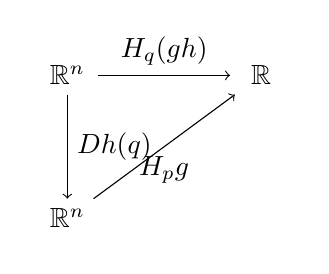
\begin{tikzpicture}
  \matrix (m) [matrix of math nodes, row sep=3.8em, column sep=4.8em, minimum width=2.2em]
  {
    \mathbb{R}^n & \mathbb{R} \\ 
     \mathbb{R}^n & \\ 
};
  \path[->]
  (m-1-1) edge node [above] {$H_q(gh) $} (m-1-2)
          edge node [auto] {$Dh(q) $} (m-2-1)
  (m-2-1) edge node [below] {$H_pg $} (m-1-2)
  ;
\end{tikzpicture}  

(quadratic) form $(H_pf)$ invariant under diffeomorphisms.


Let $C^2$ $f:M\to \mathbb{R}$.  \\
$\forall \,$ critical pt. $x$ of $f$, define \\
Hessian quadratic form
\[
\begin{aligned}
  & H_xf : M_x \to \mathbb{R} \\ 
  & H_xf : M_x \xrightarrow{ D\varphi_x } \mathbb{R}^n \xrightarrow{ H_{\varphi(x)}(f\varphi^{-1} ) } \mathbb{R}
\end{aligned}
\]
where $\varphi$ is any chart at $x$.

Thus, critical pt. of a $C^2$ real-valued function nondegenerate iff associated Hessian quadratic form is nondegenerate.  

Let $Q$ nondegenerate quadratic form on vector space $E$.

$Q$ negative definite on subspace $F \subset E$ if $Q(x)<0$ whenever $x\in F$ nonzero.

Index of $Q \equiv \text{Ind}Q$, is largest possible dim. of subspace on which $Q$ is negative definite.








cf. 1.1. Morse's Lemma of  Ch. 6, pp. 145, Morse Theory of Hirsch (1997) \cite{MHirsch1997}

\begin{lemma}[Morse's Lemma]
  Let $p\in M$ be nondegenerate critical pt. of index $k$ of $C^{r+2}$ map $f:M\to \mathbb{R}$, $1\leq r \leq \omega$.

  Then $\exists \, C^r$ chart $(\varphi,U)$ at $p$ s.t.
  \begin{equation}
    f\varphi^{-1}(u_1 \dots u_n) = f(p) - \sum_{i=1}^k u_i^2 + \sum_{i = k+1}^n u_i^2
  \end{equation}
  \end{lemma}

Let ${\,}^TQ \equiv Q^T$ denote tranpose of matrix $Q$.

\begin{lemma}
  Let $A = \text{diag}\lbrace a_1 , \dots , a_n \rbrace$ diagonal $n\times n$ matrix, with diagonal entries $\pm 1$.

  Then $\exists \, $ neighborhood $N$ of $A$ in vector space of symmetric $n\times n$ matrices, $C^{\infty}$ map
  \begin{equation}
P:N \to GL(n,\mathbb{R})
  \end{equation}
  s.t. $P(A)=I$, and if $P(B) = Q$, then $Q^T BQ = A$
\end{lemma}

\begin{proof}
  Let $B = [b_{ij}]$ be symmetri matrix near $A$ s.t. $b{11} \neq 0$ and $b_{11}$ has same sign as $a_1$.

    Consider $x=Ty$ where
    \[
\begin{aligned}
&  x_1 = \left[ y_1 - \frac{b_{12}}{b_{11}} y_2 - \dots - \frac{b_{1n}}{b_{11}} y_n \right] / \sqrt{ |b_n | } \\ 
& x_k = y_k \text{ for } k = 2, \dots n 
  \end{aligned}
    \]
  \end{proof}


\section{Lagrange multipliers}

From \emph{wikipedia:Lagrange multiplier}, \url{https://en.wikipedia.org/wiki/Lagrange_multiplier},
find local minima (maxima), pt. $a\in N$, s.t. $\exists \, $ neighborhood $U$ s.t. $f(x) \geq f(a)$ ($f(x) \leq f(a)$) \, $\forall \, x\in U$.

For $f:U\to \mathbb{R}$, open $U\subset \mathbb{R}^n$, find $x\in U$ s.t. $D_xf \equiv Df(x) =0$, check if Hessian $H_x f<0$.

Maxima may not exit since $U$ open.


References:

\href{http://www.math.uni.wroc.pl/~karch/analiza_nieliniowa/18_mnozniki-lagrangea.pdf}{Relative Extrema and Lagrange Multipliers}

Other interesting links:

\href{http://oai.cwi.nl/oai/asset/2552/2552A.pdf}{The Lagrange Multiplier Rule on Manifolds and Optimal Control of nonlinear systems}


\part{Classical Mechanics applications}

cf. Arnold, Kozlov, Neishtadt (2006) \cite{AKN2006}. 

If known forces $\mathbf{F}_1 \dots \mathbf{F}_n$ acts on points, then 
\begin{equation}
\sum_{i=1}^n \langle m_i \ddot{ \mathbf{r}}_i - \mathbf{F}_i , \mathbf{\xi}_i \rangle = 0
\end{equation}
cf. Eq. (1.26) of Arnold, Kozlov, Neishtadt (2006) \cite{AKN2006}, where $\xi_1 , \dots \xi_n$ are arbitrary tangent vectors to $M$, $\mathbf{\xi}_i, \dots \mathbf{\xi}_n \in TM$.  

$\sum_{i=1}^n \langle m_i \ddot{ \mathbf{r}}_i - \mathbf{F}_i , \mathbf{\xi}_i \rangle$ called "general equation of dynamics" or d'Alembert-Lagrange principle.  

\part{Classical Mechanics}

\section{Classical Mechanics}

\subsection{Structure of Galilean Space-Time}

cf. Sec. 3.1 - \emph{Structure of Galilean Space-Time} of Pr\'{a}staro (1996) \cite{Pras1996}.

Mechanics assumes a particular simple formulation if formulated with respect to some spacetime manifold.

In Galilean spacetime, it's possible to naturally recognize absolute objects, and others that depend on frames.

cf. Def. 3.1 of Pr\'{a}staro (1996) \cite{Pras1996}
\begin{definition}[Galilean spacetime structure]
\begin{enumerate}
	\item Galilean spacetime structure $:= (\mathcal{G}, g)$ where \\
	$\mathcal{G}$ is (fiber bundle space-time)
	\begin{equation}
		\mathcal{G} \equiv \lbrace \tau : M \to T \rbrace
	\end{equation}
	where \\
	$M = $ 4-dim. affine manifold (\textbf{space-time}); corresponding structure is $(M, \mathbf{M}, \alpha)$, \\
\item	$T = $ 1-dim. affine space (\textbf{time}), corresponding affine structure is $(T, \mathbf{T}, \beta)$
\item $\tau = $ surjective affine mapping, of constant rank $1$, s.t. $\forall \, p \in M$ associates its time $\tau(p) \in T$
\end{enumerate}

Put $\mathbf{S} = \text{ker}(\underline{\tau}) \equiv \text{ker}(D\tau)\in M$, \\
	where $\underline{\tau} \equiv D\tau$, $D$ is symbol of derivative.\\	
	Define 
	\[
	\begin{aligned}
	& g: M \to vS_2^0(M) \equiv M \times S_2^0(\mathbf{S}) \\ 
	& g(p) = (p, \underline{g})  \equiv (p, Dg) , \forall \, p \in M
	\end{aligned}
	\]
	where $\underline{g} \equiv Dg$ is a Euclidean structure on $\mathbf{S}$.  $g$ is called vertical metric field.
\end{definition}

Thus, given $(M, \mathbf{M}, \alpha)$, $\forall \, (O, \lbrace \mathbf{e}_i)_{1 \leq i \leq d}$, $\lbrace \mathbf{e}_i \rbrace_{i=1\dots d}$, is basis of $\mathbf{M}$, 
\[
M \cong \mathbb{R}^4, \text{and } \exists \, \lbrace x^{\alpha} : M = \mathbb{R}^4 \to \mathbb{R} \rbrace_{\alpha = 1 \dots 4}
\]

\subsection{Fundamental Theorems of (Classical) Dynamics}

cf. Sec. 3.4 - \emph{Fundamental Theorems of Dynamics} of Pr\'{a}staro (1996) \cite{Pras1996}.

cf. Thm. 3.20 of Pr\'{a}staro (1996) \cite{Pras1996}
\begin{theorem}[(Momentum Theorem)]
	Variation of the free part of momentum of the observed motion of 1 body, in time interval $\Delta t \equiv [0, t]$ is equal to the corresponding impulse:
	\begin{equation}
	I[0,t] \equiv \int_0^t Fdt \equiv \left( \int_0^t F^j dt \right) \mathbf{e}_j
	\end{equation}
	where $\lbrace \mathbf{e}_j \rbrace_{1 \leq j \leq 3}$ is a fixed basis of $\mathbf{S}$
	\begin{equation}
		\overline{p}_{\psi}(t) - \overline{p}_{\psi}(0) = I[0,t]
	\end{equation}
\end{theorem}

\begin{proof}
	\[
\begin{gathered}
\overline{p}_{\psi} = \mu \ddot{m}_{\psi} = \overline{f}_{\psi} \Longrightarrow \dot{ \overline{p}_{\psi}} = \dot{p}^j \mathbf{e}_j = F^j \textbf{e}_j \Longrightarrow \int_{[0,t]} \dot{p}^j dt = \int_{[0,t]}F^j dt
\end{gathered}
	\]
	\end{proof}


\end{multicols*}

\begin{thebibliography}{9}

\bibitem{Fell1968}
William Feller.  \textbf{An Introduction to Probability Theory and Its Applications}, Vol. 1, 3rd Edition.  1968.  ISBN-13: 978-0471257080



\bibitem{JLee2009}
Jeffrey M. Lee. \textbf{Manifolds and Differential Geometry}, \emph{Graduate Studies in Mathematics} Volume: 107, American Mathematical Society, 2009. ISBN-13: 978-0-8218-4815-9

\bibitem{JLee2012}
John Lee, \textbf{Introduction to Smooth Manifolds} (Graduate Texts in Mathematics, Vol. 218), 2nd edition, Springer,  2012, ISBN-13: 978-1441999818

\bibitem{VGuilleminAPollack2010}
Victor Guillemin, Alan Pollack. \textbf{Differential Topology}. American Mathematical Society. 2010. ISBN-13: 978-0821851937
\url{https://www.google.com/url?sa=t&rct=j&q=&esrc=s&source=web&cd=2&cad=rja&uact=8&ved=0ahUKEwjG96q9z63JAhWMLYgKHempDoMQFggmMAE&url=http\%3A\%2F\%2Fwww.mat.unimi.it\%2Fusers\%2Fdedo\%2Ftop\%2520diff\%2FGuillemin-Pollack_Differential\%2520topology.pdf&usg=AFQjCNF5imOH5xeXRSK60qzM7zT97sdIsw}

\bibitem{AShastri2011}
Anant R. Shastri. \textbf{Elements of Differential Topology}. CRC Press. 2011. ISBN-13: 978-0415339209

\bibitem{MHirsch1997}
Morris W. Hirsch, \textbf{Differential Topology} (Graduate Texts in Mathematics), Graduate Texts in Mathematics (Book 33), Springer (September 16, 1997). ISBN-13: 978-0387901480

\bibitem{AMS2008} 
P.-A. Absil, R. Mahony, and R. Sepulchre.  \textbf{Optimization Algorithms on Matrix Manifolds}.  Princeton University Press.  2008.  ISBN 978-0-691-13298-3
\url{https://press.princeton.edu/titles/8586.html}  

\bibitem{JBaezJMuniain1994}
John Baez, Javier P Muniain.  \textbf{Gauge Fields, Knots and Gravity} (Series on Knots and Everything), World Scientific Publishing Company (October 24, 1994), ISBN-13: 978-9810220341

\bibitem{JRotman2010}
Joseph J. Rotman, \textbf{Advanced Modern Algebra} (Graduate Studies in Mathematics), (Book 114), American Mathematical Society; 2 edition, (August 10, 2010), ISBN-13: 978-0821847411

\bibitem{ABaker2011}
Andrew Baker, ``Representations of Finite Groups'', 07112011
\url{http://www.maths.gla.ac.uk/~ajb/dvi-ps/groupreps.pdf}

\bibitem{YKosmann-Schwarzbach2010}
Yvette Kosmann-Schwarzbach, \textbf{Groups and Symmetries: From Finite Groups to Lie Groups}, Springer, 2010. e-ISBN 978-0-387-78866-1 \url{http://www.caam.rice.edu/~yad1/miscellaneous/References/Math/Groups/Groups\%20and\%20Symmetries.pdf}

\bibitem{Pras1996}
Agostino Pr\'{a}staro.  \textbf{Geometry of PDEs and Mechanics}.  World Scientific Publishing Co.  1996.  QC125.2.P73 1996  530.1'55353--dc20.  

Agostino Pr\'{a}staro.  \emph{Dipartimento di Metodi e Modelli Matematici per le Scienze Applicate, Universit\`{a} degli Studi di Roma ``La Sapienza''}.  

\bibitem{Kopp2010}
  Clemens Koppensteiner.  \emph{Complex Manifolds: Lecture Notes}.  \url{http://www.caramdir.at/uploads/math/piii-cm/complex-manifolds.pdf}
  

\bibitem{Vand2008}
Stefan Vandoren. \textbf{Lectures on Riemannian Geometry, Part II: Complex Manifolds}.  \url{http://www.staff.science.uu.nl/~vando101/MRIlectures.pdf} 

\bibitem{Hori2003}
Kentaro Hori (Author, Editor), Sheldon Katz (Editor), Albrecht Klemm (Editor), Rahul Pandharipande (Editor), Richard Thomas (Editor), Cumrun Vafa (Editor), Ravi Vakil (Editor), Eric Zaslow (Editor).  \textbf{Mirror Symmetry} (Clay Mathematics Monographs, V. 1).  Clay Mathematics Monographs (Book 1).  American Mathematical Society (August 19, 2003).  ISBN-10: 0821829556  ISBN-13: 978-0821829554  \url{https://web.archive.org/web/20060919020706/http://math.stanford.edu/~vakil/files/mirrorfinal.pdf}

\bibitem{Conl2008}
Lawrence Conlon.  \textbf{Differentiable Manifolds} (Modern Birkhäuser Classics).  2nd Edition.  Birkhäuser; 2nd edition (October 10, 2008).  ISBN-13: 978-0817647667




\bibitem{ClSa2012}
Andrew Clarke and Bianca Santoro.  \emph{Holonomy Groups in Riemannian Geometry}.  \href{https://arxiv.org/pdf/1206.3170.pdf}{arXiv:1206.3170 [math.DG]}

\bibitem{ScWa2007}
Urs Schreiber and Konrad Waldorf.  \emph{Parallel Transport and Functors}.  \href{https://arxiv.org/pdf/0705.0452.pdf}{arXiv:0705.0452 [math.DG]}

\bibitem{ElMi2002}
Y. Eliashberg, N. Mishachev, \emph{Introduction to the $h$-principle}, Grad. Studies in Math. Vol 48 (AMS 2002)


\bibitem{AKN2006}
Vladimir I. Arnold, Valery V. Kozlov, Anatoly I. Neishtadt.  \textbf{Mathematical Aspects of Classical and Celestial Mechanics}.  Third Edition.  Springer.  

\bibitem{YChoquet-Bruhat2009}
Yvonne Choquet-Bruhat.  \textbf{General Relativity and the Einstein Equations} (Oxford Mathematical Monographs) 1st Edition.  Oxford Mathematical Monographs (February 4, 2009) ISBN-13: 978-0199230723


\end{thebibliography}


\end{document}
